\documentclass[12pt,a4paper,oneside]{scrreprt}

\usepackage[T1]{fontenc}    % bessere Akzente auf äöü
\usepackage[utf8]{inputenc} 
\usepackage[ngerman]{babel} % Deutsche Begriffe
\usepackage{lmodern}        % bessere Schriftart

\usepackage{hyperref}                          % clickable links
\hypersetup{hidelinks}
\usepackage{amsmath, amssymb}                  % Mathe Formeln
\usepackage{graphicx, caption, subcaption}     % für Figures und Subfigures
\captionsetup[figure]{font=small,format=plain} % figure caption style

\usepackage{float}                             % enforce figure placement
\usepackage{setspace}                          % line double spacing...
\usepackage{geometry}
\geometry{left=3.5cm, right=2.5cm, top=2.5cm, bottom=2.5cm}

\usepackage{algorithm}
\usepackage{algorithmic}
\makeatletter \renewcommand{\ALG@name}{Algorithmus} \makeatother

% ////////////////////////////////////////////////

\begin{document}

% ////////////////////////////////////////////////

\begin{titlepage}
    \begin{figure}[H]
    \centering
    \begin{subfigure}{0.18\textwidth} 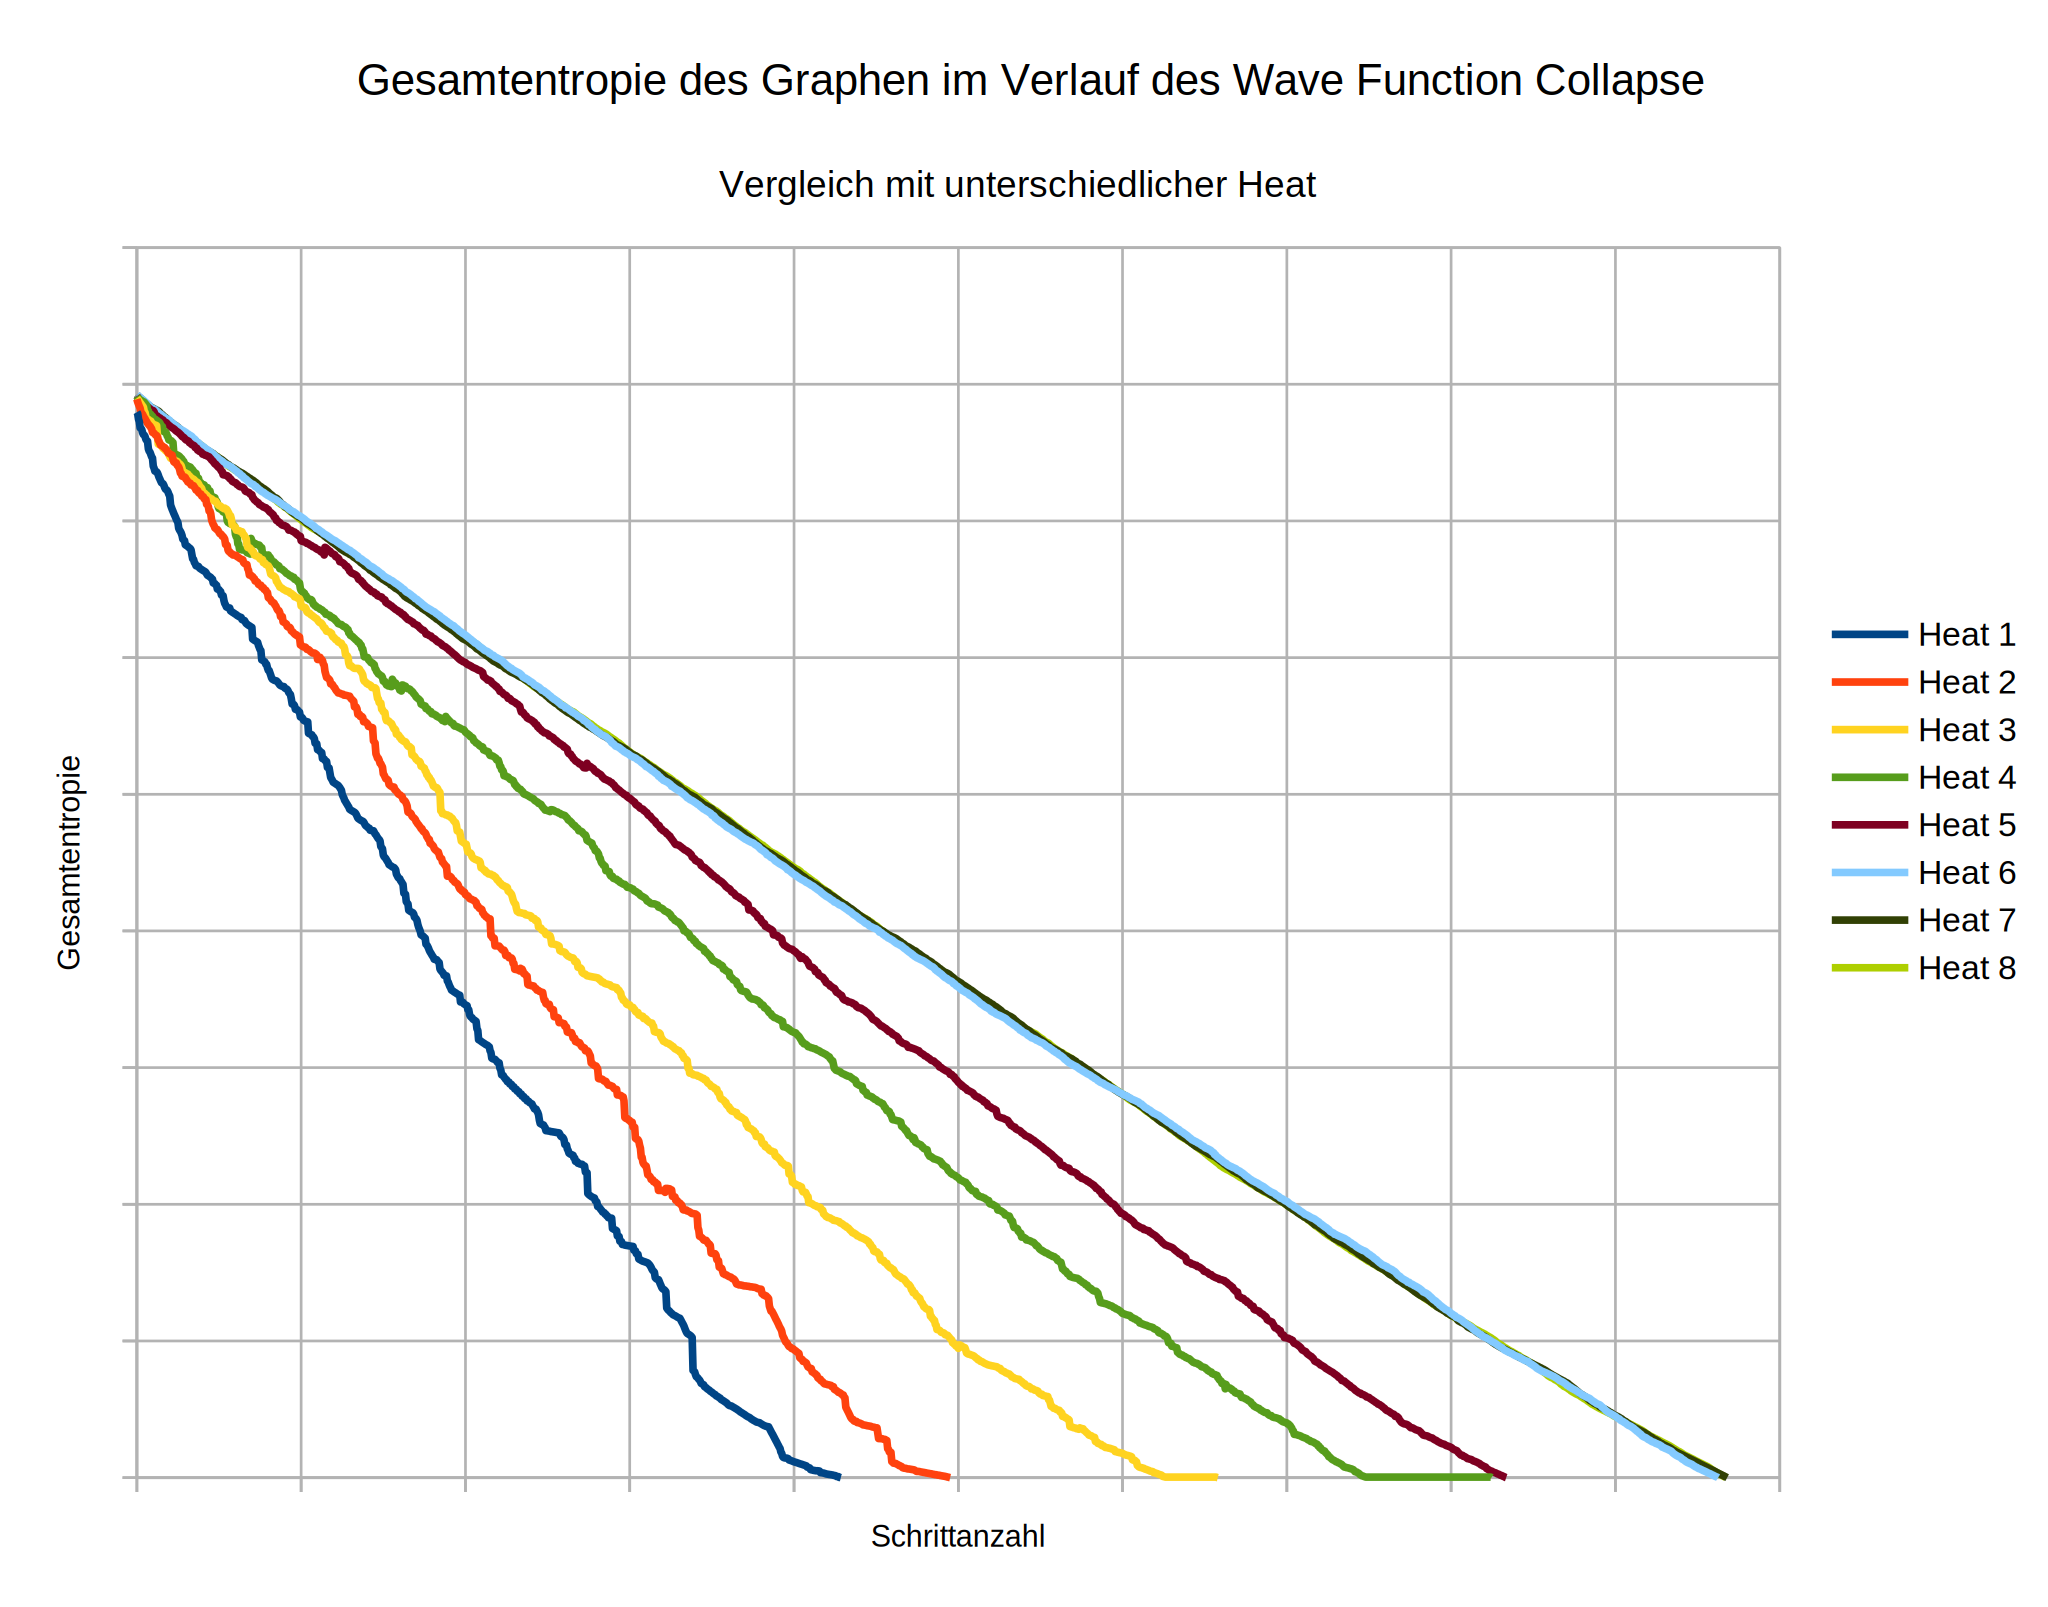
\includegraphics[width=\linewidth]{data/townscaper_grid/1.png} \caption{} \end{subfigure}
    \begin{subfigure}{0.18\textwidth} \includegraphics[width=\linewidth]{data/townscaper_grid/2.png} \caption{} \end{subfigure}
    \begin{subfigure}{0.18\textwidth} \includegraphics[width=\linewidth]{data/townscaper_grid/3.png} \caption{} \end{subfigure}
    \begin{subfigure}{0.18\textwidth} \includegraphics[width=\linewidth]{data/townscaper_grid/4.png} \caption{} \end{subfigure}
    \begin{subfigure}{0.18\textwidth} \includegraphics[width=\linewidth]{data/townscaper_grid/5.png} \caption{} \end{subfigure}
    
    \caption{
        Generierung eines Teils des Gitters für Townscaper \cite{stalberg_grid}. (a) Punkte werden generiert. (b) Triangulierung. (c) Kanten werden gelöscht, so dass Vierecke entstehen. (d) die Vierecke werden geviertelt. (e) Position der Knoten wird aufgelockert, so dass die Winkel zwischen Kanten gleichmäßiger sind.
    }
    \label{fig:townscaper_grid}
\end{figure}
    
    \begin{verbatim}
        
        
    \end{verbatim}
    
    \begin{center}
        \Large{Hochschule Anhalt}\\
        \Large{Fachbereich 5: Informatik und Sprachen}\\
    \end{center}
    
    \begin{verbatim}
        
        
    \end{verbatim}
        
    \begin{center}
        \doublespacing
        \textbf{\LARGE{Bachelorarbeit}}\\
        \begin{verbatim}
            
        \end{verbatim}
        \textbf{\LARGE{Wave Function Collapse auf Graphen}}\\
        \singlespacing
        \begin{verbatim}
            
        \end{verbatim}
    \end{center}
    \begin{verbatim}
        
        
        
    \end{verbatim}
    \begin{flushleft}
        \begin{tabular}{llll}
            \textbf{Studiengang:} & & Angewandte Informatik: Digitale Medien und Spieleentwicklung & \\
            & & \\
            \textbf{Autor:} & & Name: Viktor Graf von Westarp & \\
            & & Matrikelnummer: 5058639 & \\
            & & \\
            \textbf{Abgabedatum:} & & 5.\,Dezember\,2025 &\\
            & & \\
            \textbf{Betreuer:} & & Prof.\,Dr.\,Stefan Schlechtweg &\\
            \textbf{Zweitgutachterin:} & & Prof.\,Dr.\,Anika Groß &\\
        \end{tabular}
    \end{flushleft}
\end{titlepage}



% ////////////////////////////////////////////////

\tableofcontents

% ////////////////////////////////////////////////



\chapter*{Zusammenfassung}
\begin{quote}

Es wird eine Erweiterung des \textit{Wave Function Collapse} Algorithmus präsentiert, die aus einem Beispiel ähnliche Ausgaben nicht nur wie zuvor auf regelmäßigen Gittern, sondern nun auch auf beliebigen Graphen prozedural generieren kann. 
Die unterliegenden Struktur der Ausgabe wird von der Struktur des Beispiel entkoppelt und es können komplexere oder gar zuvor unmögliche, Ausgaben erstellt werden, ohne dass das Beispiel für diese angepasst werden muss. 
Ein neues Konzept namens \textit{Heat} definiert, wie der Algorithmus die aus dem Beispiel extrahierten Regeln auf die Knoten des Graphen und deren Nachbarknoten anwendet. Dadurch können die Knoten beliebig angeordnet werden, anstatt auf ein Gitter beschränkt zu sein. Des weiteren wird Backtracking in der Generierung eingeführt, um die Laufzeit zu verbessern. Es wird auch gezeigt, wie die für die Ausgabe genutzten Graphen automatisch erzeugt werden.
Der erweiterte Algorithmus kann mit demselben Beispiel erfolgreich eine Vielzahl an Ausgaben auf unterschiedlichen Graphen generieren. Die Qualität der generierten Ausgabe hängt zu gleichen Teilen von dem Beispiel, dem Graphen und der gewählten Heat ab. Diese Beziehung wird genauer untersucht.
Es wurde sich auf zweidimensionale Graphen beschränkt. Außerdem ist Heat als globaler, graph-weiter Wert definiert. Dies macht die Methode besonders geeignet für Graphen mit relativ gleichmäßig verteilten Knoten. Bei stark unregelmäßigen Graph-Strukturen scheitert der Algorithmus häufiger oder kann nie eine zufriedenstellende Ausgabe generieren.

\end{quote}





\chapter{Einleitung}
    Dieses Kapitel erklärt zuerst die Motivation hinter dieser Arbeit und geht auf das zu lösende Problem und das genaue Ziel dieser Arbeit ein. Danach wird ein Überblick über den Aufbau der Arbeit gegeben.
    
    \section{Motivation}
        Wave Function Collapse ist ein spannender Algorithmus, der, basiert auf einem einzigen Beispielmodell oder -bild, eine große Menge an ähnlichen Modellen und Bildern prozedural generieren kann. Bisher bestimmte die Form des Beispiels auch die Form der Ausgabe. Ein Beispielbild besteht aus Pixeln, also werden auch Bilder aus Pixeln generiert. Auch bei 3D-Modellen beschränkt sich der Nutzer meist auf  z.B. würfelförmige Bauteile, aus denen dann ein Modell zusammengestellt wird. Auch wenn der Innenbereich solcher Bauteile beliebige Formen haben kann, werden die Bauteile dennoch würfelförmig aneinandergereiht.
        
        Es muss aber nicht so sein, denn der Algorithmus selbst ist agnostisch gegenüber der Form der Ein- und Ausgabe. Es können nicht nur Bilder, sondern auch 3D-Modelle generiert werden. Es sollte also möglich sein, dass der Algorithmus die Muster in einem Beispielbild auch auf eine anders geformte Struktur replizieren kann. Genauer sollte die Ausgabe nicht nur auf einem Gitter, sondern nun auch auf Graphen, geschehen können.
        
        Wäre dies möglich, so könnten Nutzer mit dem Algorithmus beliebige Strukturen als Basis nutzen und wären nicht mehr auf reine Gitter beschränkt. Dadurch könnten unregelmäßige oder organische Anordnungen, wie sie z.B. in der Natur, historischen Städten oder einem Mosaik vorkommen, als Basis für Ausgaben genutzt werden.
    
    
    
    \section{Problemstellung und Ziel}
        Ziel dieser Arbeit ist es, den Wave Function Collapse Algorithmus so zu erweitern, dass dieser eine Ausgabe auf Graphen generieren kann. Das heißt, dass die Struktur der Eingabe nicht mehr exakt zur Struktur der Ausgabe passen muss, sondern dass z.B. ein Beispielbild auf unterschiedlich strukturierte Graphen anwendbar sein soll, ohne dass das Beispielbild dafür verändert werden muss. 
        
        Das Kernproblem dabei ist, wie genau der Algorithmus die Informationen aus dem Beispielbild auf die Knoten eines Graphen einheitlich anwenden kann, wenn die Anordnung der Knoten und die Anzahl der Kanten pro Knoten im Graphen stark variieren können und keinerlei Ähnlichkeit zum Pixelgitter eines Bilds haben müssen. Gleichzeitig sollte der erweiterte Algorithmus immer noch die gleiche Qualität für Ausgaben auf Gittern, als spezielle Art von Graphen, beibehalten. Insgesamt sollen die generierten Ausgaben eine gewisse Ähnlichkeit zum Beispiel haben, wobei diese vielleicht abgeschwächt werden muss. Dennoch sollte der Algorithmus eine hohe Ähnlichkeit erzielen.
    
    
    
    \section{Aufbau der Arbeit}
        Es folgen fünf Kapitel in dieser Arbeit. Zuerst werden grundlegende Begriffe erklärt, und es wird ein Überblick über den Stand der Technik im Bereich des Wave Function Collapse gegeben. Danach wird die Beschränkung des Algorithmus genauer beschrieben und darauf eingegangen wie der Algorithmus erweitert wird und welchen Änderungen es dafür bedarf. Danach wird erklärt, wie diese Änderungen umgesetzt wurden. Es folgt ein Überblick über die erzielten Resultate und es wird genauer auf Aspekte der Erweiterung eingegangen. Schließlich folgt eine Zusammenfassung der Arbeit, in der auch auf die Vor- und Nachteile eingegangen wird.




\chapter{Hintergrund}
    In diesem Kapitel werden zuerst einige grundlegende Begriffe erklärt. Danach wird auf die Algorithmen eingegangen, auf denen diese Arbeit basiert. Dies sind \textit{Model Synthesis} von Merrel \cite{merrel} und dessen Weiterentwicklung \textit{Wave Function Collapse} von Gumin \cite{gumin}.
    
    \section{Begriffserklärung}
        Ein \textit{Gitter} beschreibt eine regelmäßig aufgebaute Struktur aus einzelnen Punkten. Diese Knotenpunkte sind durch Kanten mit ihren direkten Nachbarn verbunden. Ein Bild wird digital z.B. auf einem Gitter von Pixeln gespeichert und dargestellt. Genauso bilden die Kästchen eines Sudoku ein Gitter. Wenn solch ein Gitter in einer Ebene liegt, wird es auch als \textit{2D Gitter} bezeichnet. Sind die Punkte regelmäßig im Raum angeordnet, spricht man von einem \textit{3D Gitter}. Ein \textit{Graph} besteht aus einer Menge an Knoten $V$ und einer Menge an Kanten $E$, wobei eine Kante ein Knotenpaar aus $V$ ($\{v_1, v_2\} \in V$) ist. Die Knotenpunkte können eine beliebige Anordnung haben und beliebig mit anderen Knoten durch Kanten verbunden sein. Ein Gitter ist eine spezielle Form eines Graphen, bei dem die Knoten entlang fester Achsen angeordnet werden und nur Kanten entlang dieser Achsen zu den nächstliegenden Knoten existieren.
        \\
        \\
        Eine \textit{Triangulierung} ist ein Graph, dessen Knoten und Kanten Dreiecke aufspannen. Eine besonders wichtige Variante ist die \textit{Delaunay-Triangulierung} \cite{delaunay}, bei der die Dreiecke so gewählt werden, dass der kleinste Winkel innerhalb jedes Dreiecks möglichst groß ist. Dadurch entstehen „gut geformte“ Dreiecke. Eng verwandt damit ist das \textit{Voronoi-Diagramm} \cite{voronoi}. Es teilt die Ebene in Regionen auf, sodass jeder Punkt genau die Fläche erhält, die ihm am nächsten liegt. Die Delaunay-Triangulierung und das Voronoi-Diagramm sind dual zueinander: Verbindet man die Mittelpunkte der Voronoi-Zellen, entsteht die Delaunay-Triangulierung, und aus einer Delaunay-Triangulierung lässt sich wiederum das zugehörige Voronoi-Diagramm ableiten. In Abbildung \ref{fig:delaunay_voronoi} sind die Delaunay-Triangulierung und das Voronoi-Diagramm für einige Punkte dargestellt.
        
        \begin{figure}[H]
    \centering
    \begin{subfigure}{0.18\textwidth} 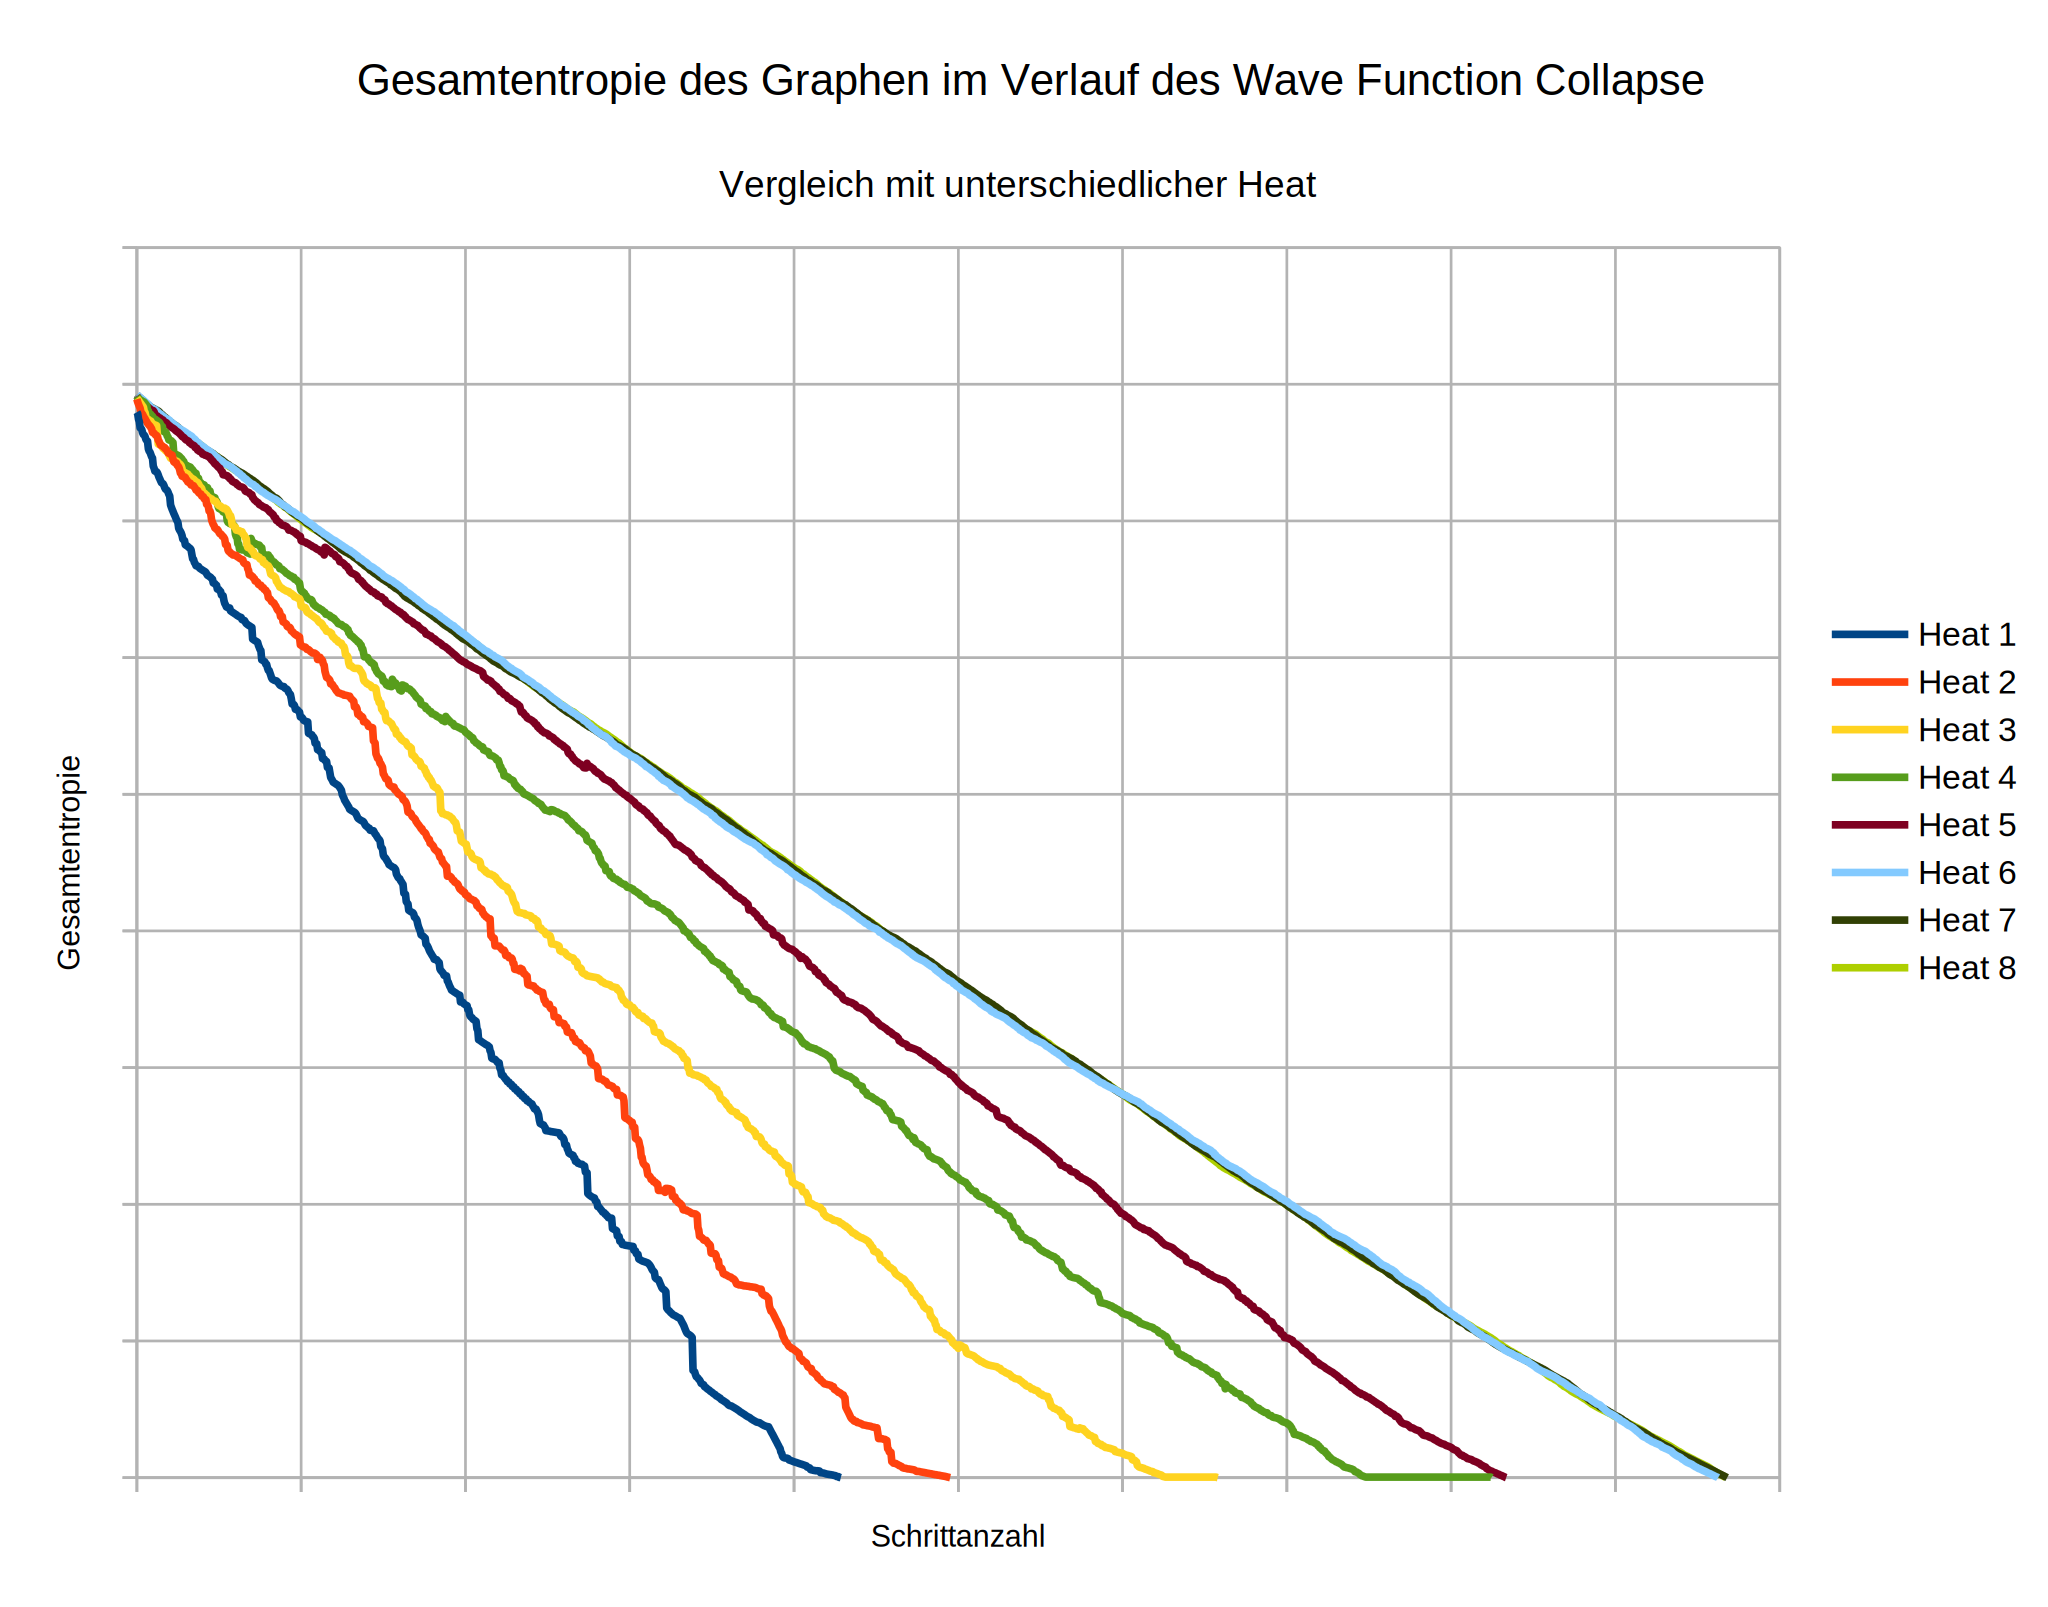
\includegraphics[width=\linewidth]{data/townscaper_grid/1.png} \caption{} \end{subfigure}
    \begin{subfigure}{0.18\textwidth} \includegraphics[width=\linewidth]{data/townscaper_grid/2.png} \caption{} \end{subfigure}
    \begin{subfigure}{0.18\textwidth} \includegraphics[width=\linewidth]{data/townscaper_grid/3.png} \caption{} \end{subfigure}
    \begin{subfigure}{0.18\textwidth} \includegraphics[width=\linewidth]{data/townscaper_grid/4.png} \caption{} \end{subfigure}
    \begin{subfigure}{0.18\textwidth} \includegraphics[width=\linewidth]{data/townscaper_grid/5.png} \caption{} \end{subfigure}
    
    \caption{
        Generierung eines Teils des Gitters für Townscaper \cite{stalberg_grid}. (a) Punkte werden generiert. (b) Triangulierung. (c) Kanten werden gelöscht, so dass Vierecke entstehen. (d) die Vierecke werden geviertelt. (e) Position der Knoten wird aufgelockert, so dass die Winkel zwischen Kanten gleichmäßiger sind.
    }
    \label{fig:townscaper_grid}
\end{figure}
        
        Unter \textit{Prozeduraler Generierung} versteht man Algorithmen, die Inhalte wie z.B. Bilder, 3D-Modelle oder Musik erzeugen können. Meist nimmt ein solcher Algorithmus nur eine kleine Menge an Daten als Eingabe und generiert daraus viele Variationen an Ausgaben. Dabei werden häufig Zufallszahl-Generatoren benutzt, aber der Ablauf ist nicht rein zufällig. Bei gleicher Initialisierung generiert ein solcher Algorithmus immer dieselbe Ausgabe und kann durch Parameter gesteuert werden. Prozedurale Generierung wird in Computerspielen regelmäßig verwendet, da es den Entwicklern erlaubt, den Spielern viele variierte Inhalte zu bieten, ohne diese alle vorher manuell anzufertigen und fest im Spiel einzubauen.
    
    \section{Model Synthesis}
        Mit dem \textit{Model Synthesis} \cite{merrel} Algorithmus (siehe Algorithmus \ref{alg:ms_merrel}) können basierend auf einem 3D Beispielmodell eine große Menge an ähnlichen 3D-Modellen prozedural generiert werden (siehe Abbildung \ref{fig:ms_output}). Das Beispielmodell muss zuvor in kleinere Bauteile zerlegt werden, aus denen der Algorithmus dann ein neues Modell generiert. Ein Bauteil kann ein komplexer Teil des Beispiels sein, kann aber auch einen leeren Teil des Beispiels enthalten. Die Bauteile werden wie Bauklötze zusammengebaut, wobei zwei Bauteile nur dann nebeneinander platziert werden dürfen, wenn diese auch im Beispielmodell nebeneinander vorkommen. Diese Eigenschaft wird auch Konsistenz genannt. Ein simples konsistentes Modell ist z.B. ein leeres Modell.
        
        Der Algorithmus arbeitet auf einem 3D Gitter. Jedem Knotenpunkt des Gitters wird im fertigen Modell ein Bauteil zugewiesen, doch vorher könnten an jedem Knotenpunkt mehrere Bauteile ein konsistentes Modell bilden. Der Algorithmus wählt iterativ ein Bauteil und prüft, dass dadurch kein anderer Knotenpunkt nun keine möglichen Bauteile mehr hat. Wäre dies der Fall, so könnte das Modell nicht mehr vervollständigt werden. Hierfür wird eine globale Suche verwendet; andere Methoden beschränkten sich zuvor nur auf lokale Suchen. Eine globale Suche hat den Vorteil, dass auch ein weitreichender Einfluss eines Bauteils auf das gesamte Gitter korrekt behandelt wird. Die Auswahl der Bauteile geschieht per Zufall, dabei werden Bauteile die oft im Beispiel vorkommen wahrscheinlicher ausgewählt als seltene Bauteile. Für ein generiertes Modell bedeutet dies, dass die globale Verteilung der Bauteile auch tendenziell der Verteilung im Beispiel gleicht.
        
        \begin{figure}[H]
    \centering
    \begin{subfigure}{0.18\textwidth} 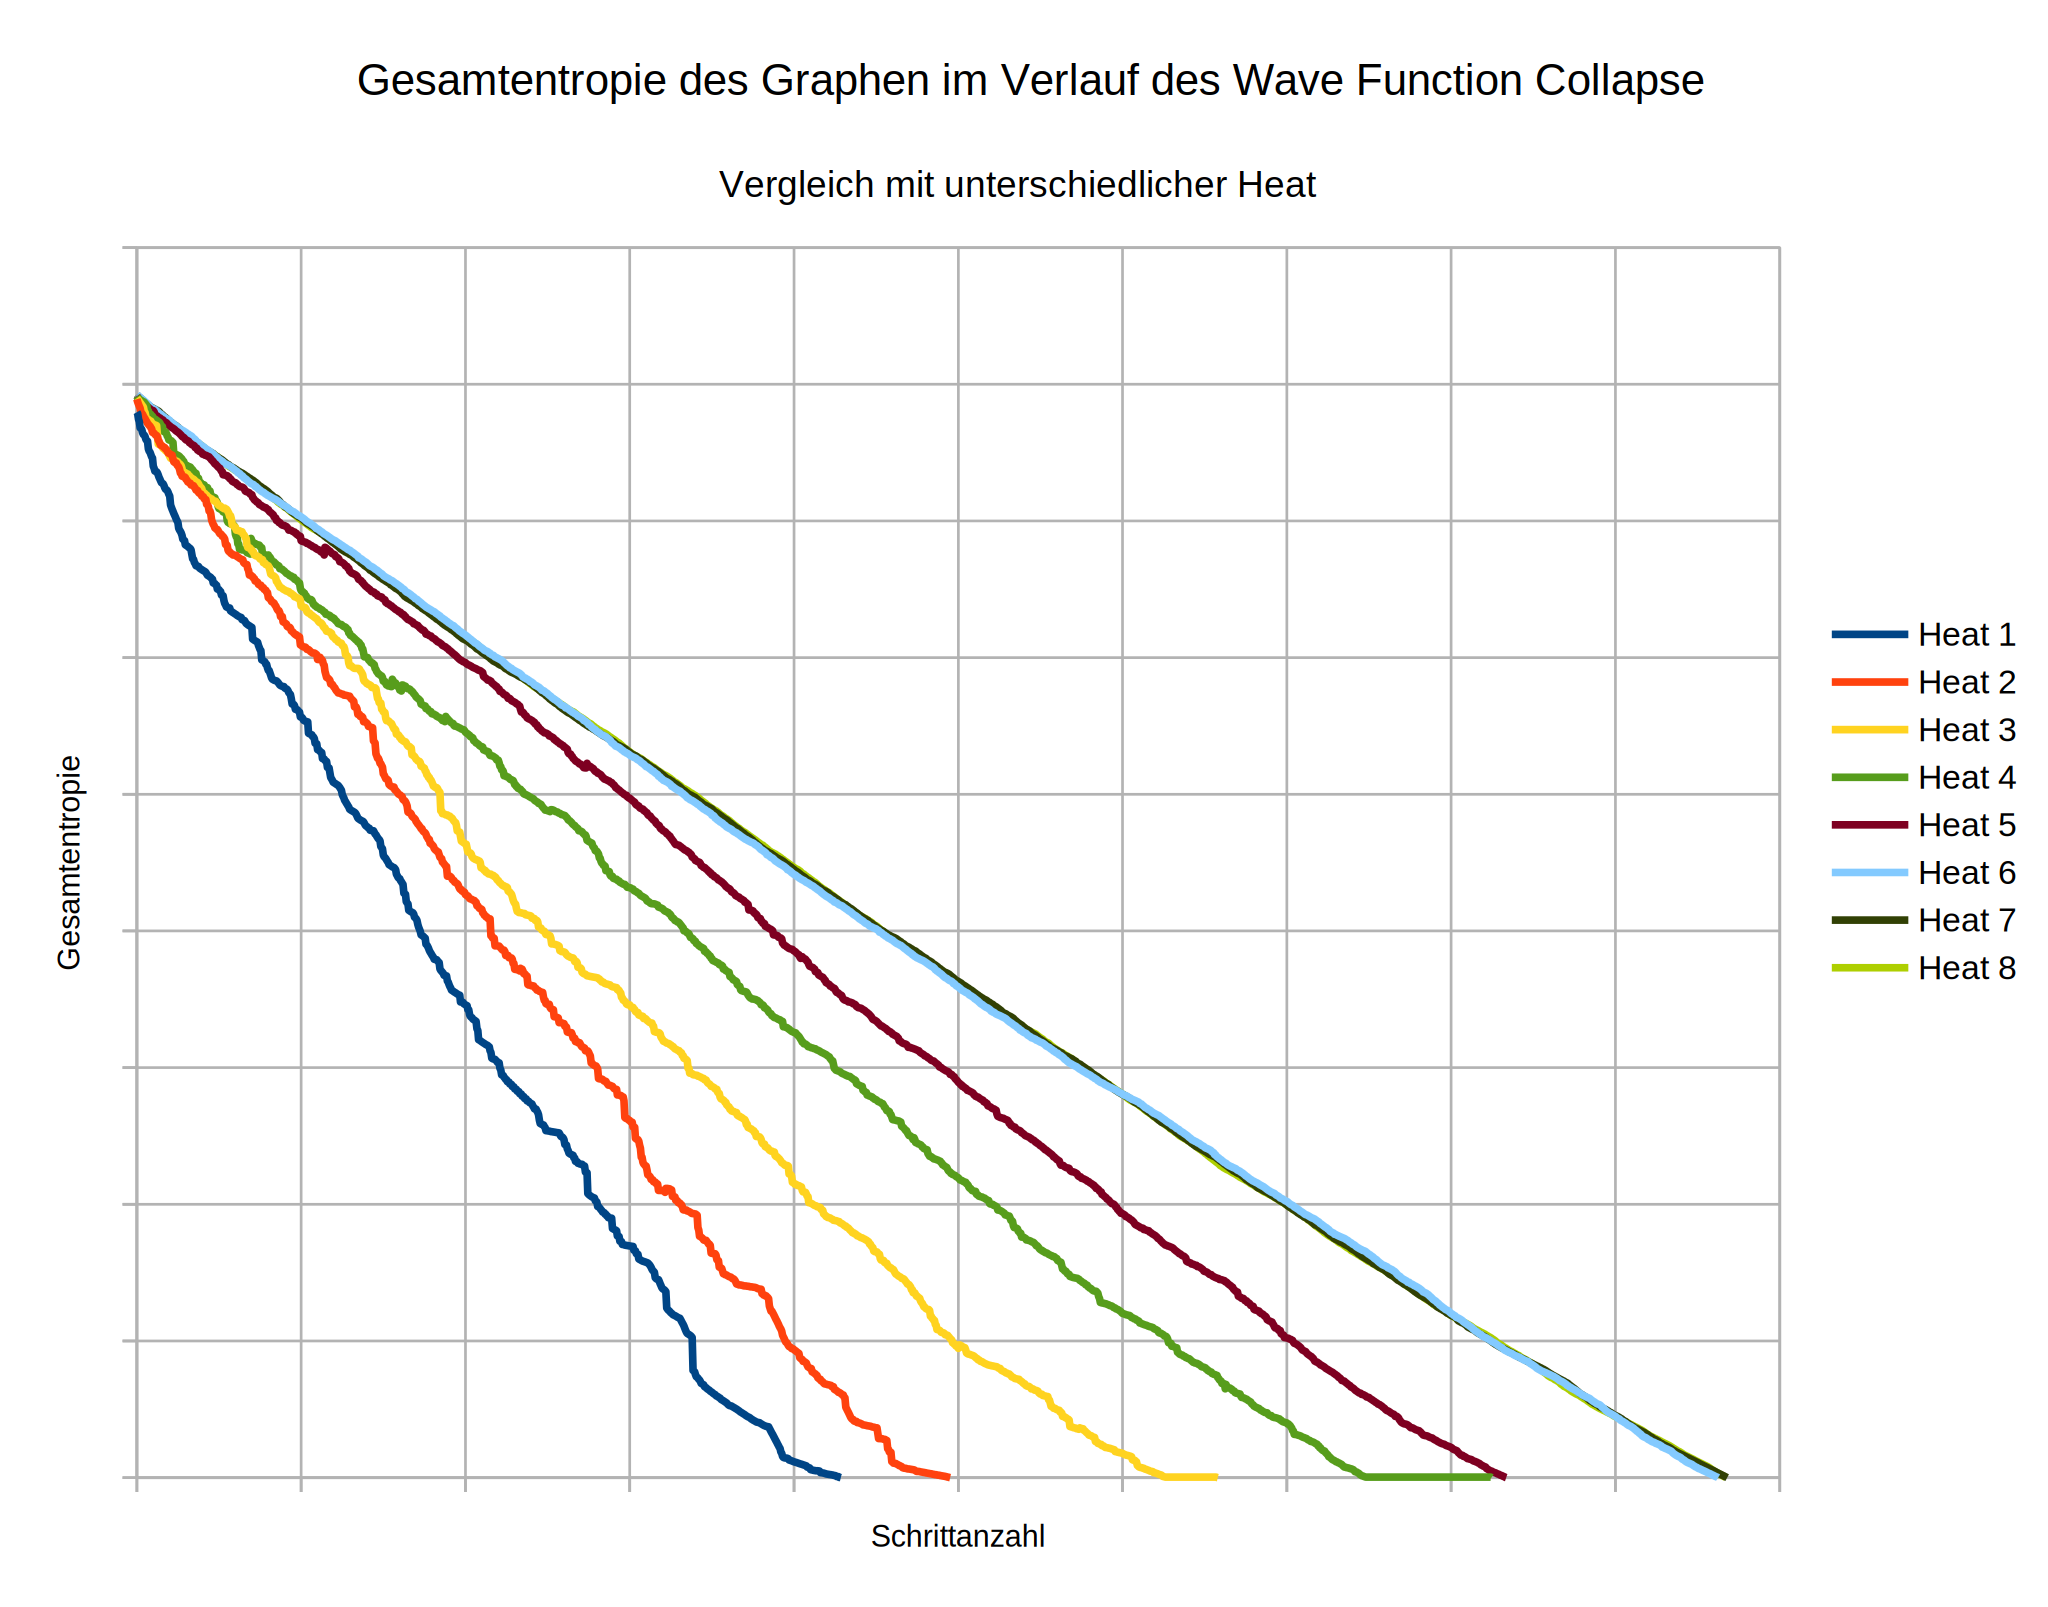
\includegraphics[width=\linewidth]{data/townscaper_grid/1.png} \caption{} \end{subfigure}
    \begin{subfigure}{0.18\textwidth} \includegraphics[width=\linewidth]{data/townscaper_grid/2.png} \caption{} \end{subfigure}
    \begin{subfigure}{0.18\textwidth} \includegraphics[width=\linewidth]{data/townscaper_grid/3.png} \caption{} \end{subfigure}
    \begin{subfigure}{0.18\textwidth} \includegraphics[width=\linewidth]{data/townscaper_grid/4.png} \caption{} \end{subfigure}
    \begin{subfigure}{0.18\textwidth} \includegraphics[width=\linewidth]{data/townscaper_grid/5.png} \caption{} \end{subfigure}
    
    \caption{
        Generierung eines Teils des Gitters für Townscaper \cite{stalberg_grid}. (a) Punkte werden generiert. (b) Triangulierung. (c) Kanten werden gelöscht, so dass Vierecke entstehen. (d) die Vierecke werden geviertelt. (e) Position der Knoten wird aufgelockert, so dass die Winkel zwischen Kanten gleichmäßiger sind.
    }
    \label{fig:townscaper_grid}
\end{figure}
        \begin{figure}[H]
    \centering
    \begin{minipage}{\linewidth}
        \rule{\linewidth}{0.4pt}
         
        \begin{enumerate}
        \item $M_0$ ist ein simples konsitentes Modell. $M = M_0$
        \subitem Wiederhole 2. bis 5. bis jeder Teil des Modells angepasst wurde
        \item Wähle eine Menge $B$ an Knotenpunkten zur Bearbeitung
        \item  $M' = M$ ohne die Knotenpunkte $B$ und deren bisherigen Bauteilen
        \item Arbeite alle Knotenpunkte von $B$ ab:
        \subitem Wähle einen Knotenpunkte aus und weise ihm ein konsistentes Bauteil zu
        \subitem Ist $M'$ nicht mehr konsistent, dann brich ab
        \subitem Füge diesen Knotenpunkt in $M'$ ein
        \item Wenn $M'$ noch konsistent ist, dann $M = M'$
        \end{enumerate}
        
        \rule{\linewidth}{0.4pt}
    \end{minipage}
    
    \caption{Model Synthesis Algorithmus nach Merrel \cite{merrel}}
    
    \label{fig:ms_merrel}
\end{figure}
        \begin{figure}[H]
    \centering
    \begin{subfigure}{0.18\textwidth} 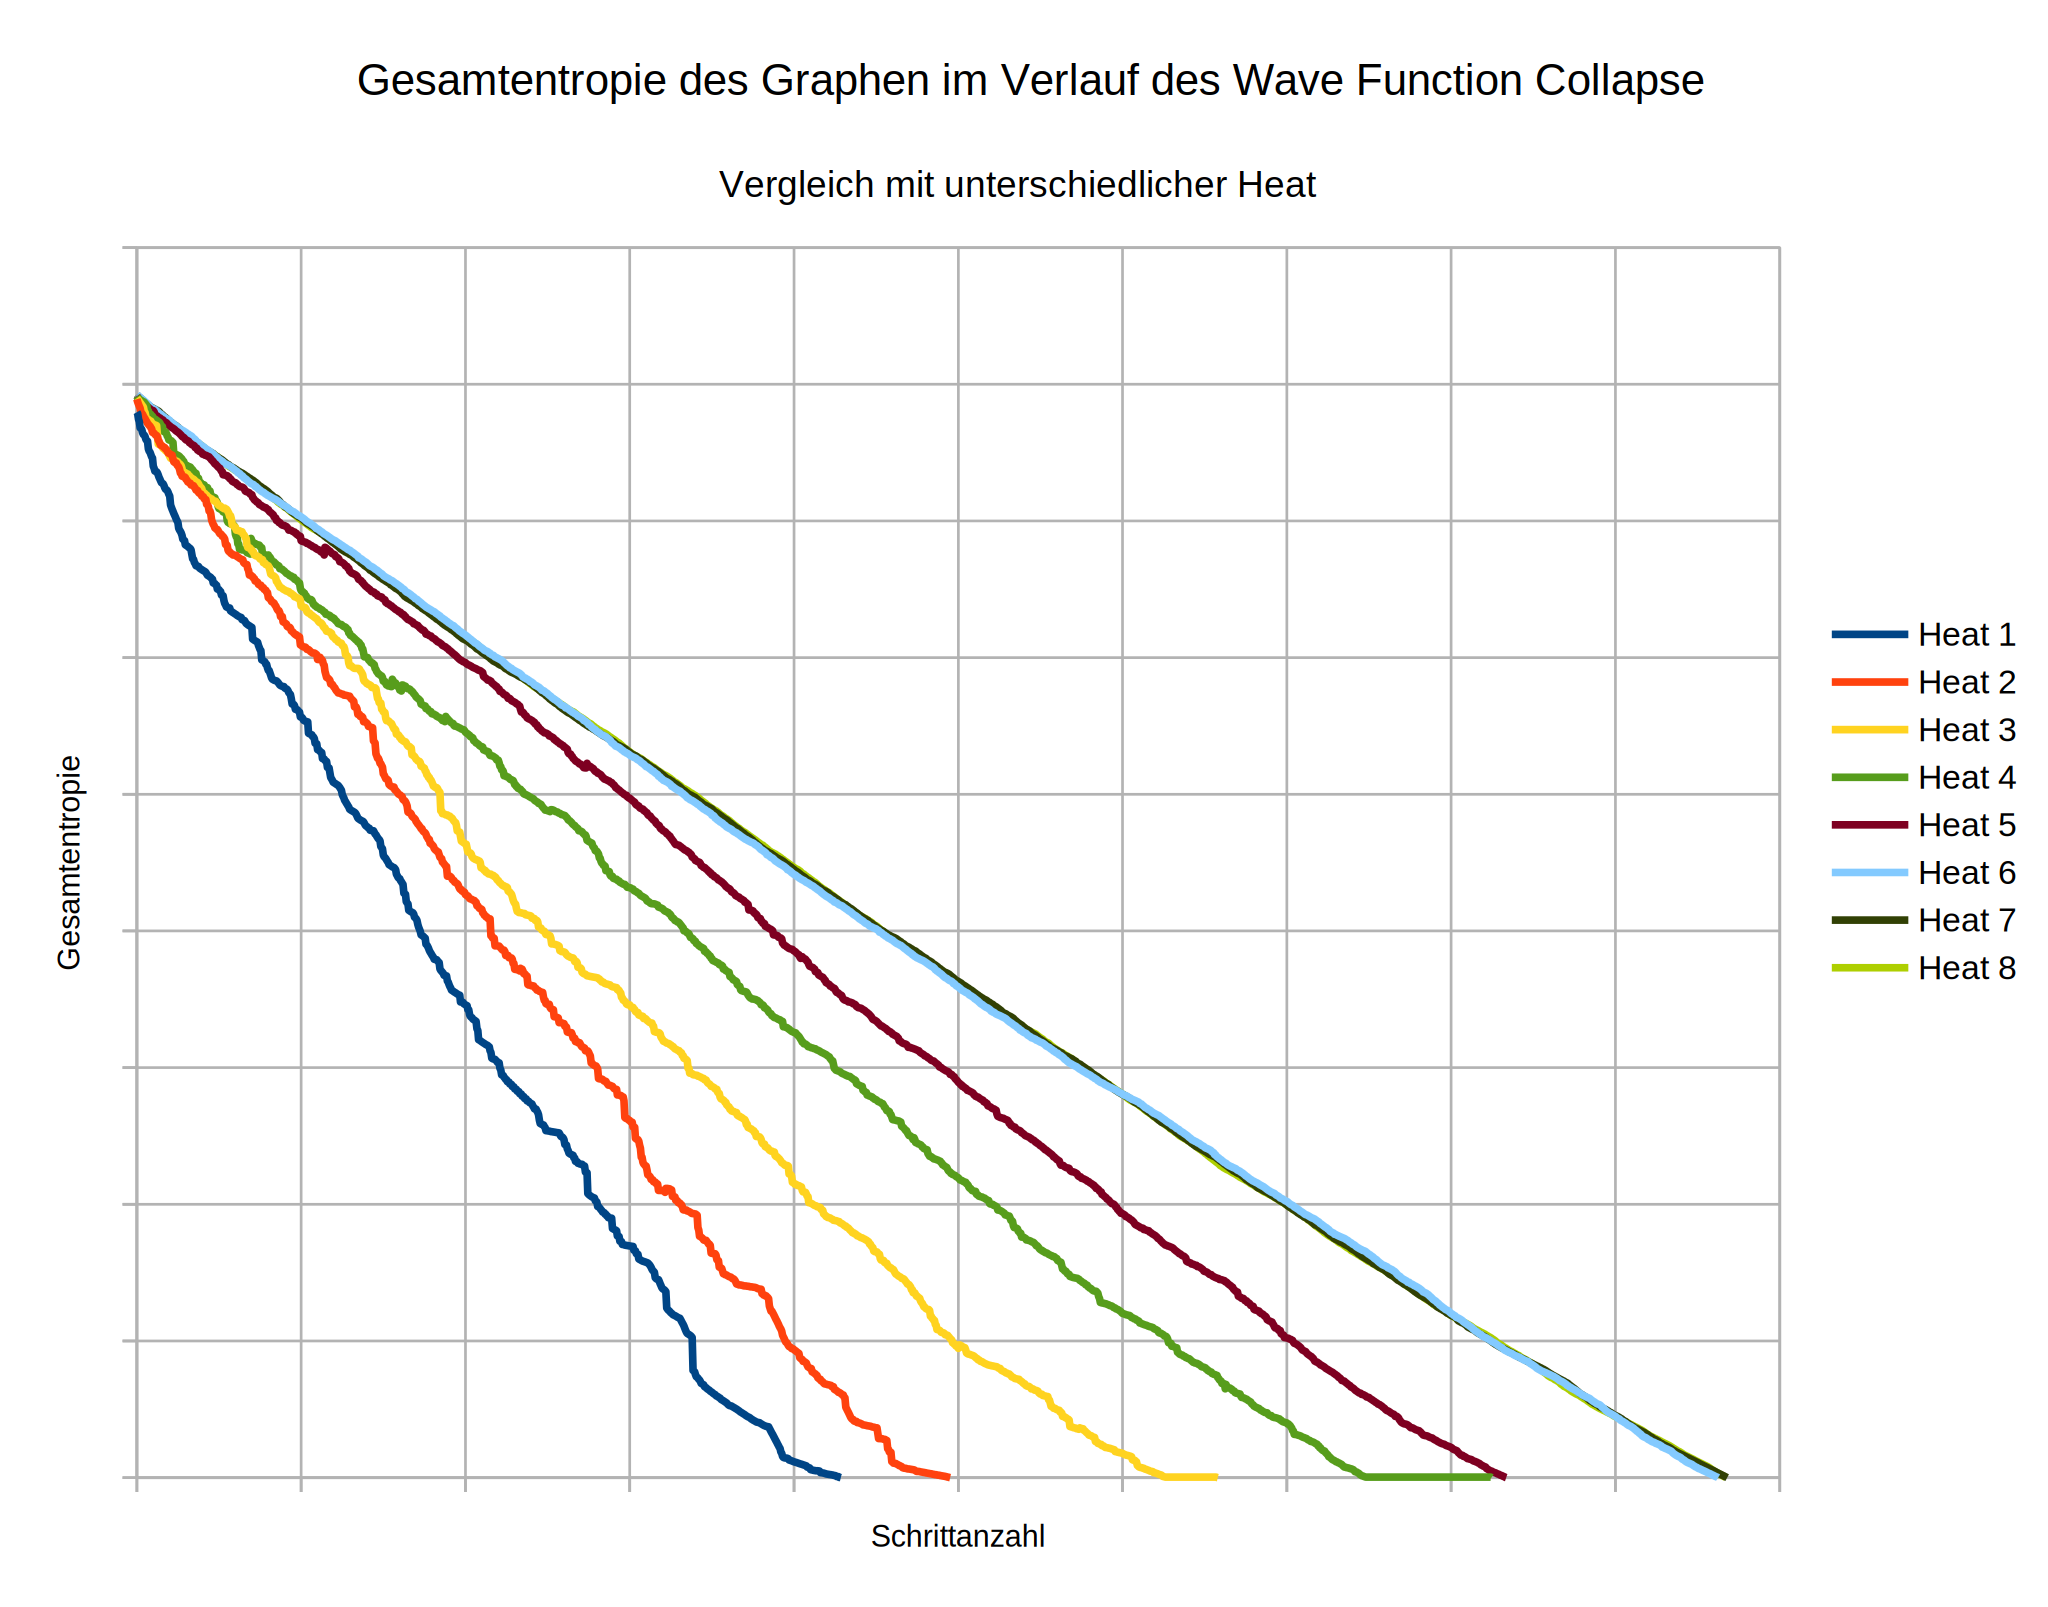
\includegraphics[width=\linewidth]{data/townscaper_grid/1.png} \caption{} \end{subfigure}
    \begin{subfigure}{0.18\textwidth} \includegraphics[width=\linewidth]{data/townscaper_grid/2.png} \caption{} \end{subfigure}
    \begin{subfigure}{0.18\textwidth} \includegraphics[width=\linewidth]{data/townscaper_grid/3.png} \caption{} \end{subfigure}
    \begin{subfigure}{0.18\textwidth} \includegraphics[width=\linewidth]{data/townscaper_grid/4.png} \caption{} \end{subfigure}
    \begin{subfigure}{0.18\textwidth} \includegraphics[width=\linewidth]{data/townscaper_grid/5.png} \caption{} \end{subfigure}
    
    \caption{
        Generierung eines Teils des Gitters für Townscaper \cite{stalberg_grid}. (a) Punkte werden generiert. (b) Triangulierung. (c) Kanten werden gelöscht, so dass Vierecke entstehen. (d) die Vierecke werden geviertelt. (e) Position der Knoten wird aufgelockert, so dass die Winkel zwischen Kanten gleichmäßiger sind.
    }
    \label{fig:townscaper_grid}
\end{figure}
        
        Die gleiche Methodik kann auch für Beispielbilder verwendet werden; dies wird dann auch \textit{Texture Synthesis} genannt. In diesem Fall arbeitet der Algorithmus mit 2D Gittern und Bauteilen. Die Ausgabe des Algorithmus kann auch durch Soft-Constraints beschränkt werden (siehe Abbildung \ref{fig:ms_constrained}). Ebenso kann Symmetrie, Spiegelung und Drehung, in der Ausgabe erzwungen werden. Beide Ansätze wurden nicht weiter in dieser Arbeit betrachtet. Es wird empfohlen, dass der Algorithmus nicht das ganze Gitter auf einmal löst, damit Widersprüche nicht zu einem kompletten Neustart führen. Stattdessen sollen iterativ kleine Abschnitte für sich solange gelöst werden, bis eine valide Ausgabe entsteht (siehe Abbildung \ref{fig:ms_algorithm}). In dieser Arbeit wurde darauf verzichtet.
        
        \begin{figure}[H]
    \centering
    \begin{subfigure}{0.18\textwidth} 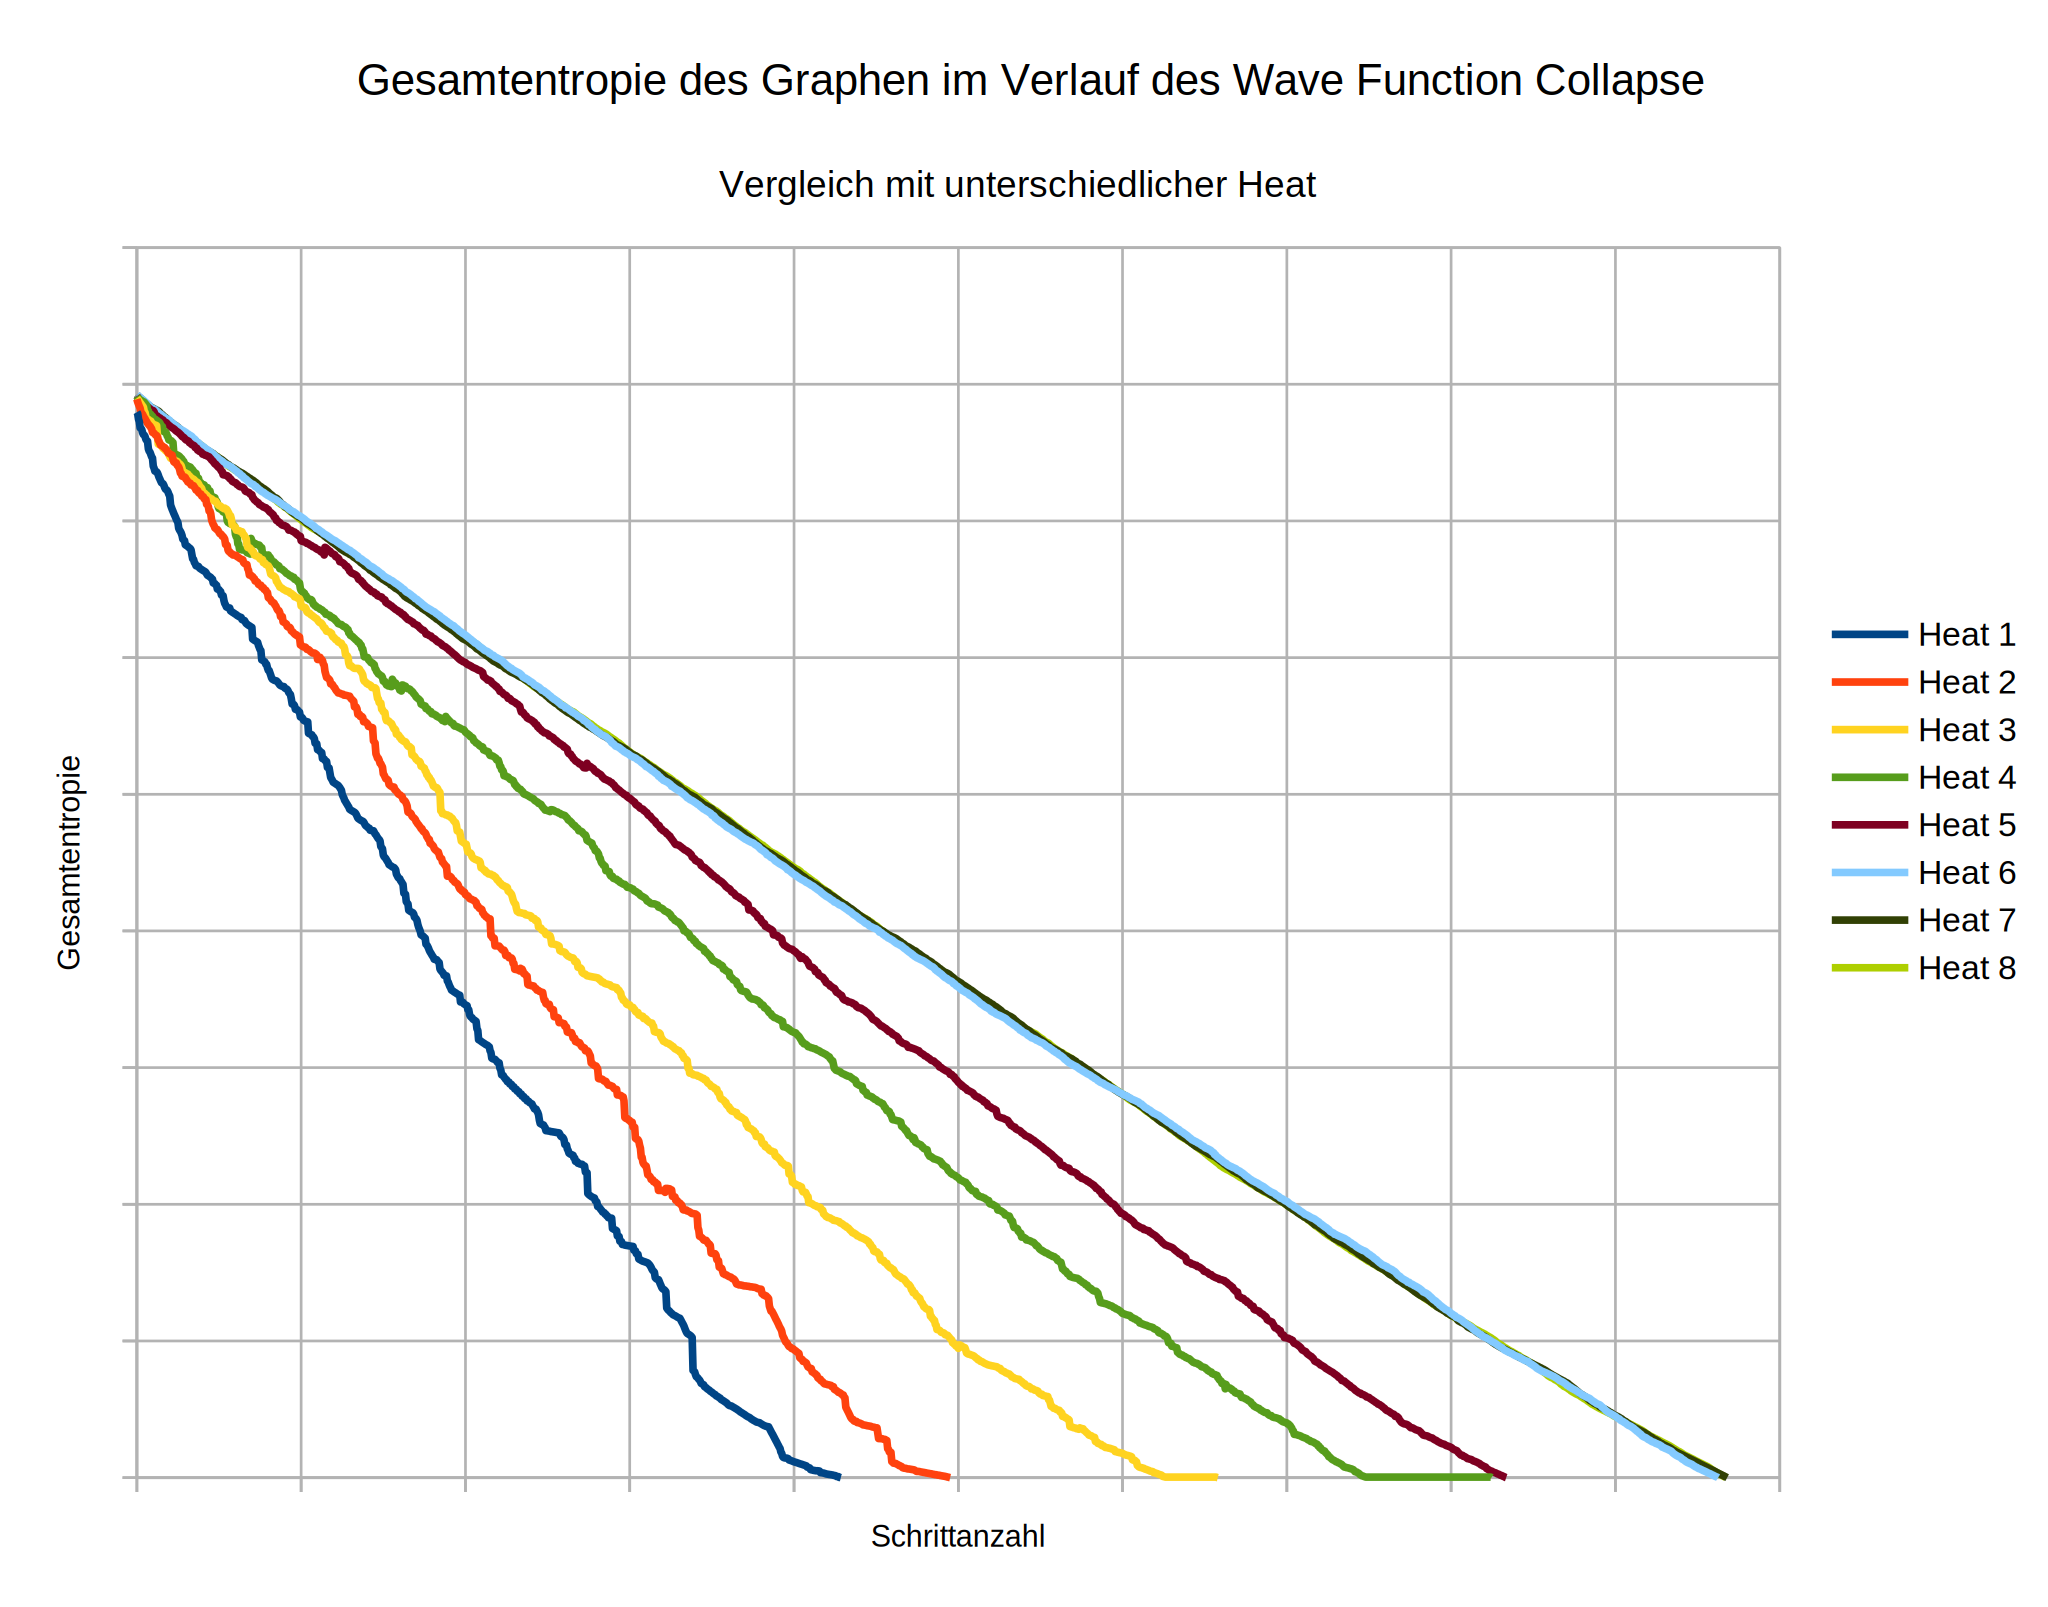
\includegraphics[width=\linewidth]{data/townscaper_grid/1.png} \caption{} \end{subfigure}
    \begin{subfigure}{0.18\textwidth} \includegraphics[width=\linewidth]{data/townscaper_grid/2.png} \caption{} \end{subfigure}
    \begin{subfigure}{0.18\textwidth} \includegraphics[width=\linewidth]{data/townscaper_grid/3.png} \caption{} \end{subfigure}
    \begin{subfigure}{0.18\textwidth} \includegraphics[width=\linewidth]{data/townscaper_grid/4.png} \caption{} \end{subfigure}
    \begin{subfigure}{0.18\textwidth} \includegraphics[width=\linewidth]{data/townscaper_grid/5.png} \caption{} \end{subfigure}
    
    \caption{
        Generierung eines Teils des Gitters für Townscaper \cite{stalberg_grid}. (a) Punkte werden generiert. (b) Triangulierung. (c) Kanten werden gelöscht, so dass Vierecke entstehen. (d) die Vierecke werden geviertelt. (e) Position der Knoten wird aufgelockert, so dass die Winkel zwischen Kanten gleichmäßiger sind.
    }
    \label{fig:townscaper_grid}
\end{figure}
    
    
    \section{Wave Function Collapse}
        \textit{Wave Function Collapse} \cite{gumin} ist eine Weiterentwicklung des Model Synthesis Algorithmus (siehe Algorithmus \ref{alg:wfc_gumin}). Abbildung \ref{fig:wfc_overview} zeigt einige Beispiele und daraus generierte Bilder. Der Name ist eine Anspielung auf die Quantenphysik. So könnte man Quantenpartikel in Superposition mit den Zellen des Gitters vergleichen. Die Zellen haben auch mehrere mögliche finale Zustände, bis sie observiert werden und in einen festen Zustand kollabiert. Mathematisch besteht aber keine Beziehung. Außerdem werden andere Begriffe, wie z.B. Knoten, zu Zelle umbenannt und das Gitter als Wave bezeichnet. Die Kernidee der Generierung mittels eines Beispiels bleibt und wird um drei Aspekte erweitert:
        
        \begin{enumerate}
        \item Bauteile können automatisch aus einem Beispiel extrahiert werden.
        \item Im Algorithmus werden die Zellen beginnend mit der niedrigsten Entropie abgearbeitet. 
        \item Spiegelungen und Reflexionen von Bauteilen werden automatisch erzeugt und verwendet.
        \end{enumerate}
        
        \begin{figure}[ht]
    \centering
    \begin{minipage}{\linewidth}
        \rule{\linewidth}{0.4pt}
        
        \begin{enumerate}
        \item Read the input bitmap and count NxN patterns.
        \subitem (optional) Augment pattern data with rotations and reflections.
        \item Create an array with the dimensions of the output (called ''wave'' in the source). Each element of this array represents a state of an NxN region in the output. A state of an NxN region is a superposition of NxN patterns of the input with boolean coefficients (so a state of a pixel in the output is a superposition of input colors with real coefficients). False coefficient means that the corresponding pattern is forbidden, true coefficient means that the corresponding pattern is not yet forbidden.
        \item Initialize the wave in the completely unobserved state, i.e. with all the boolean coefficients being true.
        \item Repeat the following steps: \begin{enumerate}
            \item Observation: \begin{enumerate}
                \item Find a wave element with the minimal nonzero entropy. If there is no such elements (if all elements have zero or undefined entropy) then break the cycle (4) and go to step (5).
                \item Collapse this element into a definite state according to its coefficients and the distribution of NxN patterns in the input.
            \end{enumerate}
            \item Propagation: propagate information gained on the previous observation step.
        \end{enumerate}
        \item By now all the wave elements are either in a completely observed state (all the coefficients except one being zero) or in the contradictory state (all the coefficients being zero). In the first case return the output. In the second case finish the work without returning anything.
        \end{enumerate}
        
        \rule{\linewidth}{0.4pt}
    \end{minipage}
    
    \caption{Wave Function Collapse Algorithmus nach Gumin \cite{gumin}}
    
    \label{fig:wfc_gumin}
\end{figure}
        \begin{figure}[H]
    \centering
    \begin{subfigure}{0.18\textwidth} 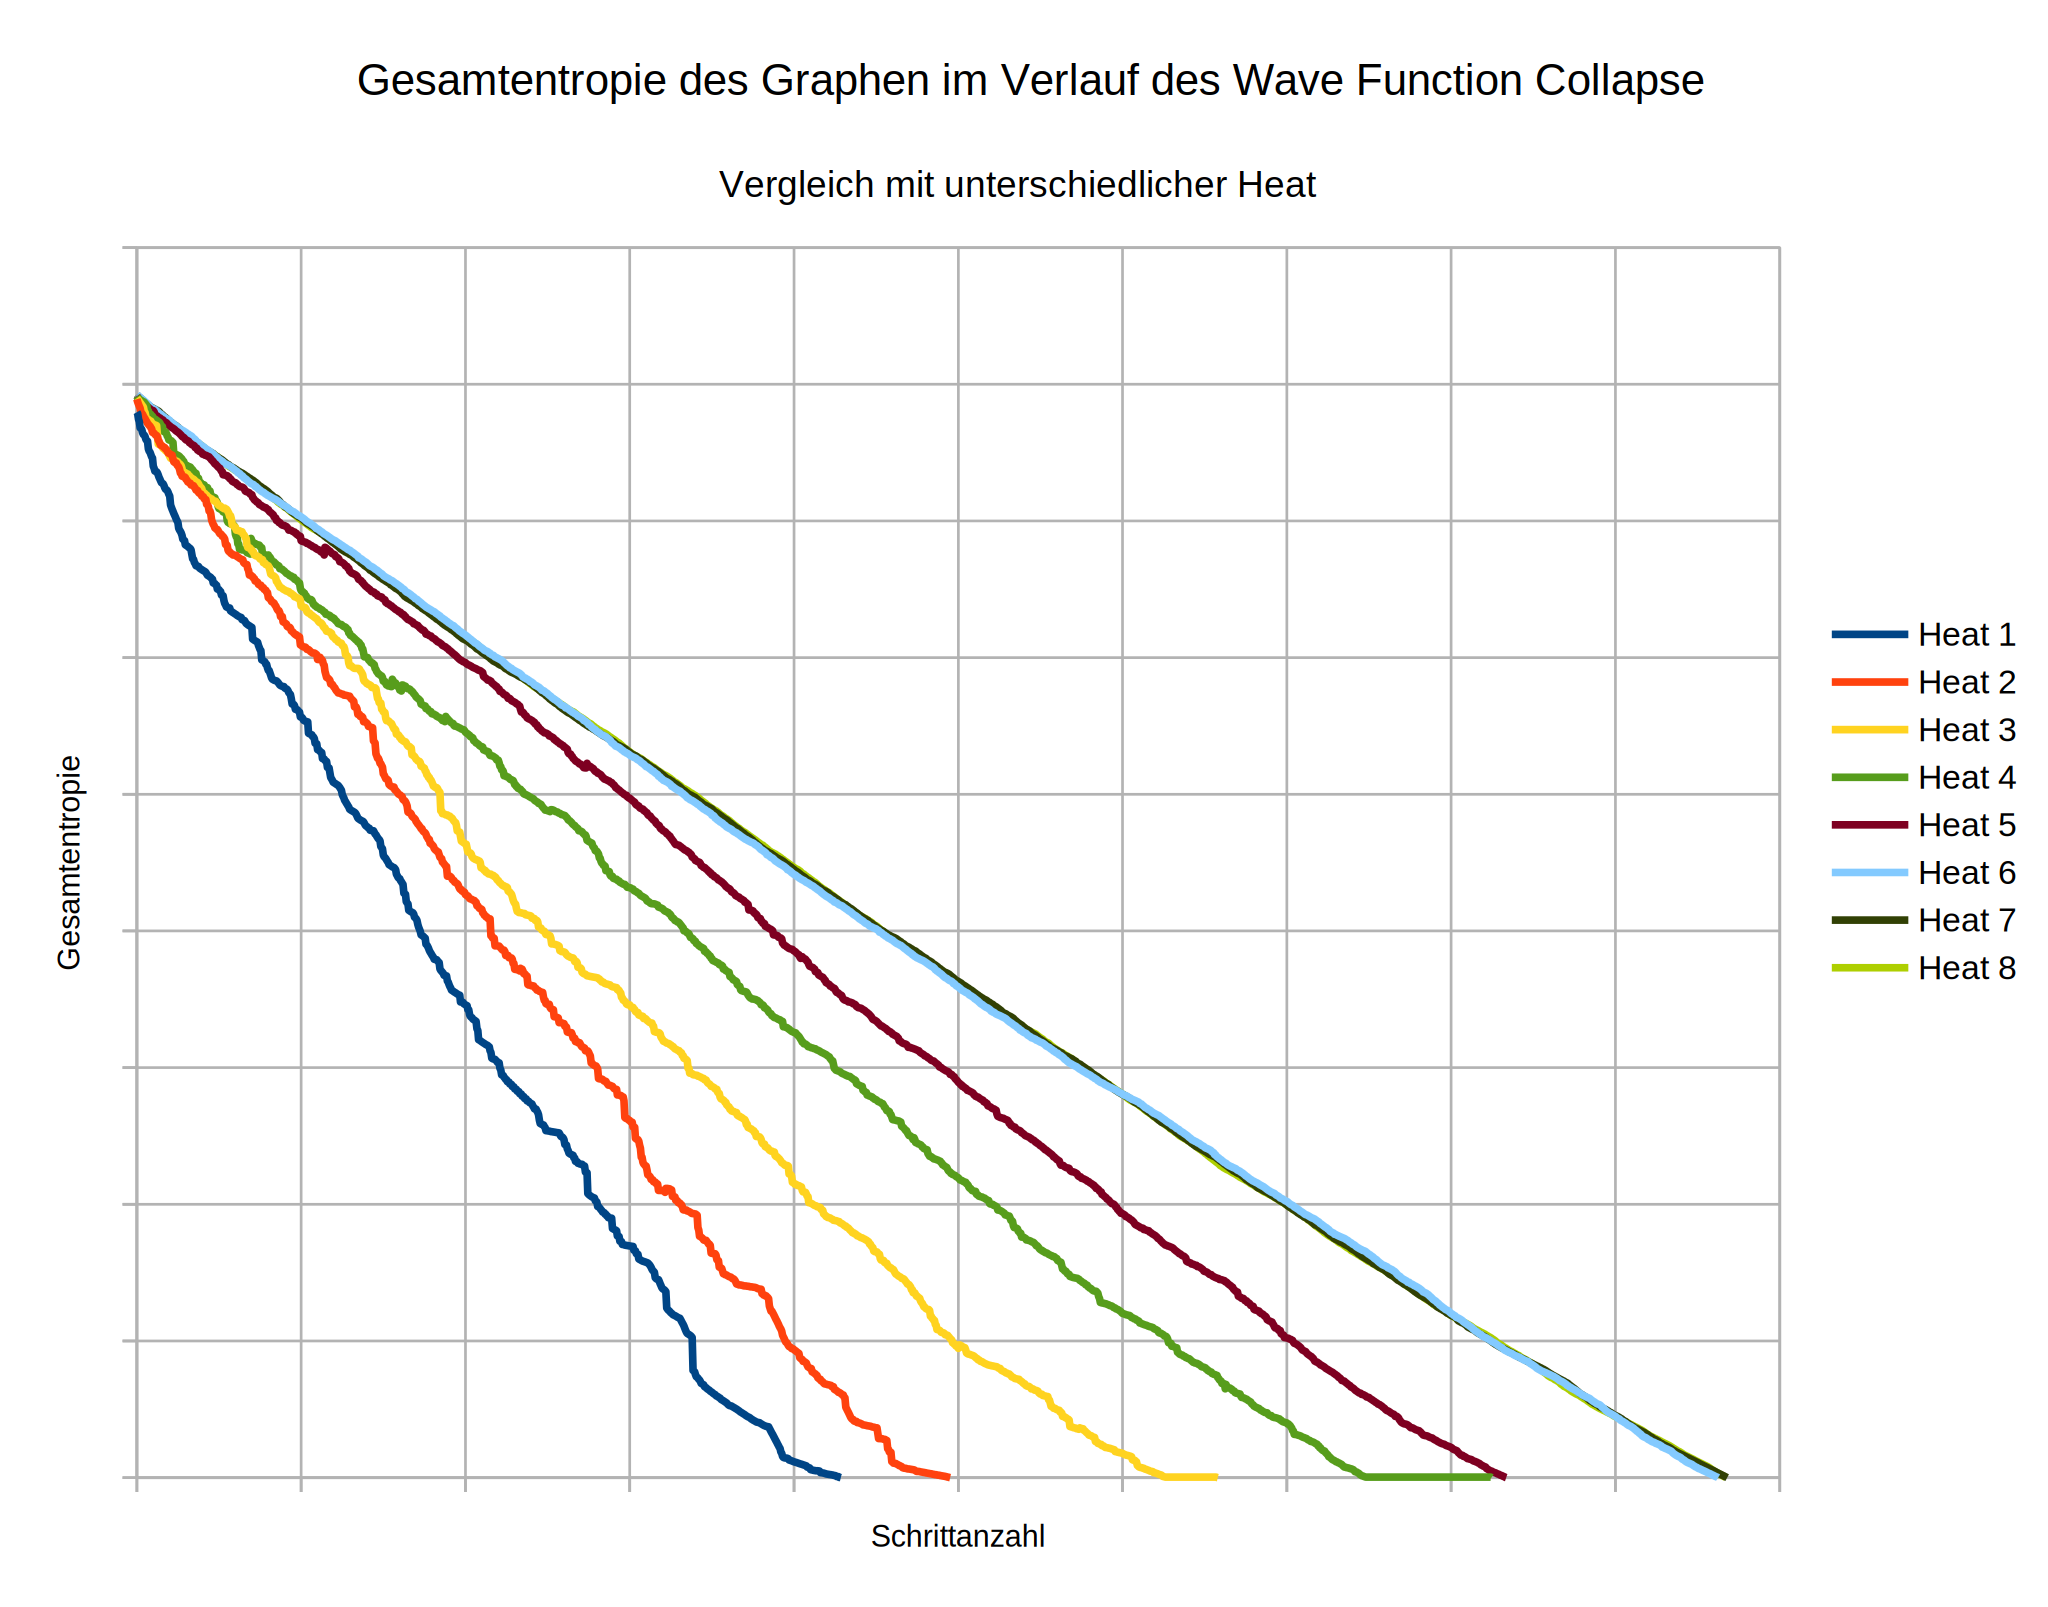
\includegraphics[width=\linewidth]{data/townscaper_grid/1.png} \caption{} \end{subfigure}
    \begin{subfigure}{0.18\textwidth} \includegraphics[width=\linewidth]{data/townscaper_grid/2.png} \caption{} \end{subfigure}
    \begin{subfigure}{0.18\textwidth} \includegraphics[width=\linewidth]{data/townscaper_grid/3.png} \caption{} \end{subfigure}
    \begin{subfigure}{0.18\textwidth} \includegraphics[width=\linewidth]{data/townscaper_grid/4.png} \caption{} \end{subfigure}
    \begin{subfigure}{0.18\textwidth} \includegraphics[width=\linewidth]{data/townscaper_grid/5.png} \caption{} \end{subfigure}
    
    \caption{
        Generierung eines Teils des Gitters für Townscaper \cite{stalberg_grid}. (a) Punkte werden generiert. (b) Triangulierung. (c) Kanten werden gelöscht, so dass Vierecke entstehen. (d) die Vierecke werden geviertelt. (e) Position der Knoten wird aufgelockert, so dass die Winkel zwischen Kanten gleichmäßiger sind.
    }
    \label{fig:townscaper_grid}
\end{figure}
        \pagebreak
        
        \subsection{Entropie}
            Bei Model Synthesis werden Zellen einfach nach ihrer Reihenfolge im Gitter abgearbeitet. Der Vorteil ist, dass keine Suche nach der nächsten Zelle nötig ist, aber es hat den Nachteil, dass die Ausgabe sichtbare Artefakte enthält (siehe Abbildung \ref{fig:directional_bias}). Man kann erkennen, ob zuerst die Reihen oder erst die Spalten abgearbeitet wurden. Wäre bekannt, welche Zelle den größten Fortschritt zur Lösung und die geringste Chance auf einen Widerspruch birgt, könnte stets diese Zelle zuerst betrachtet werden. 
            
            \begin{figure}[H]
    \centering
    \begin{subfigure}{0.18\textwidth} 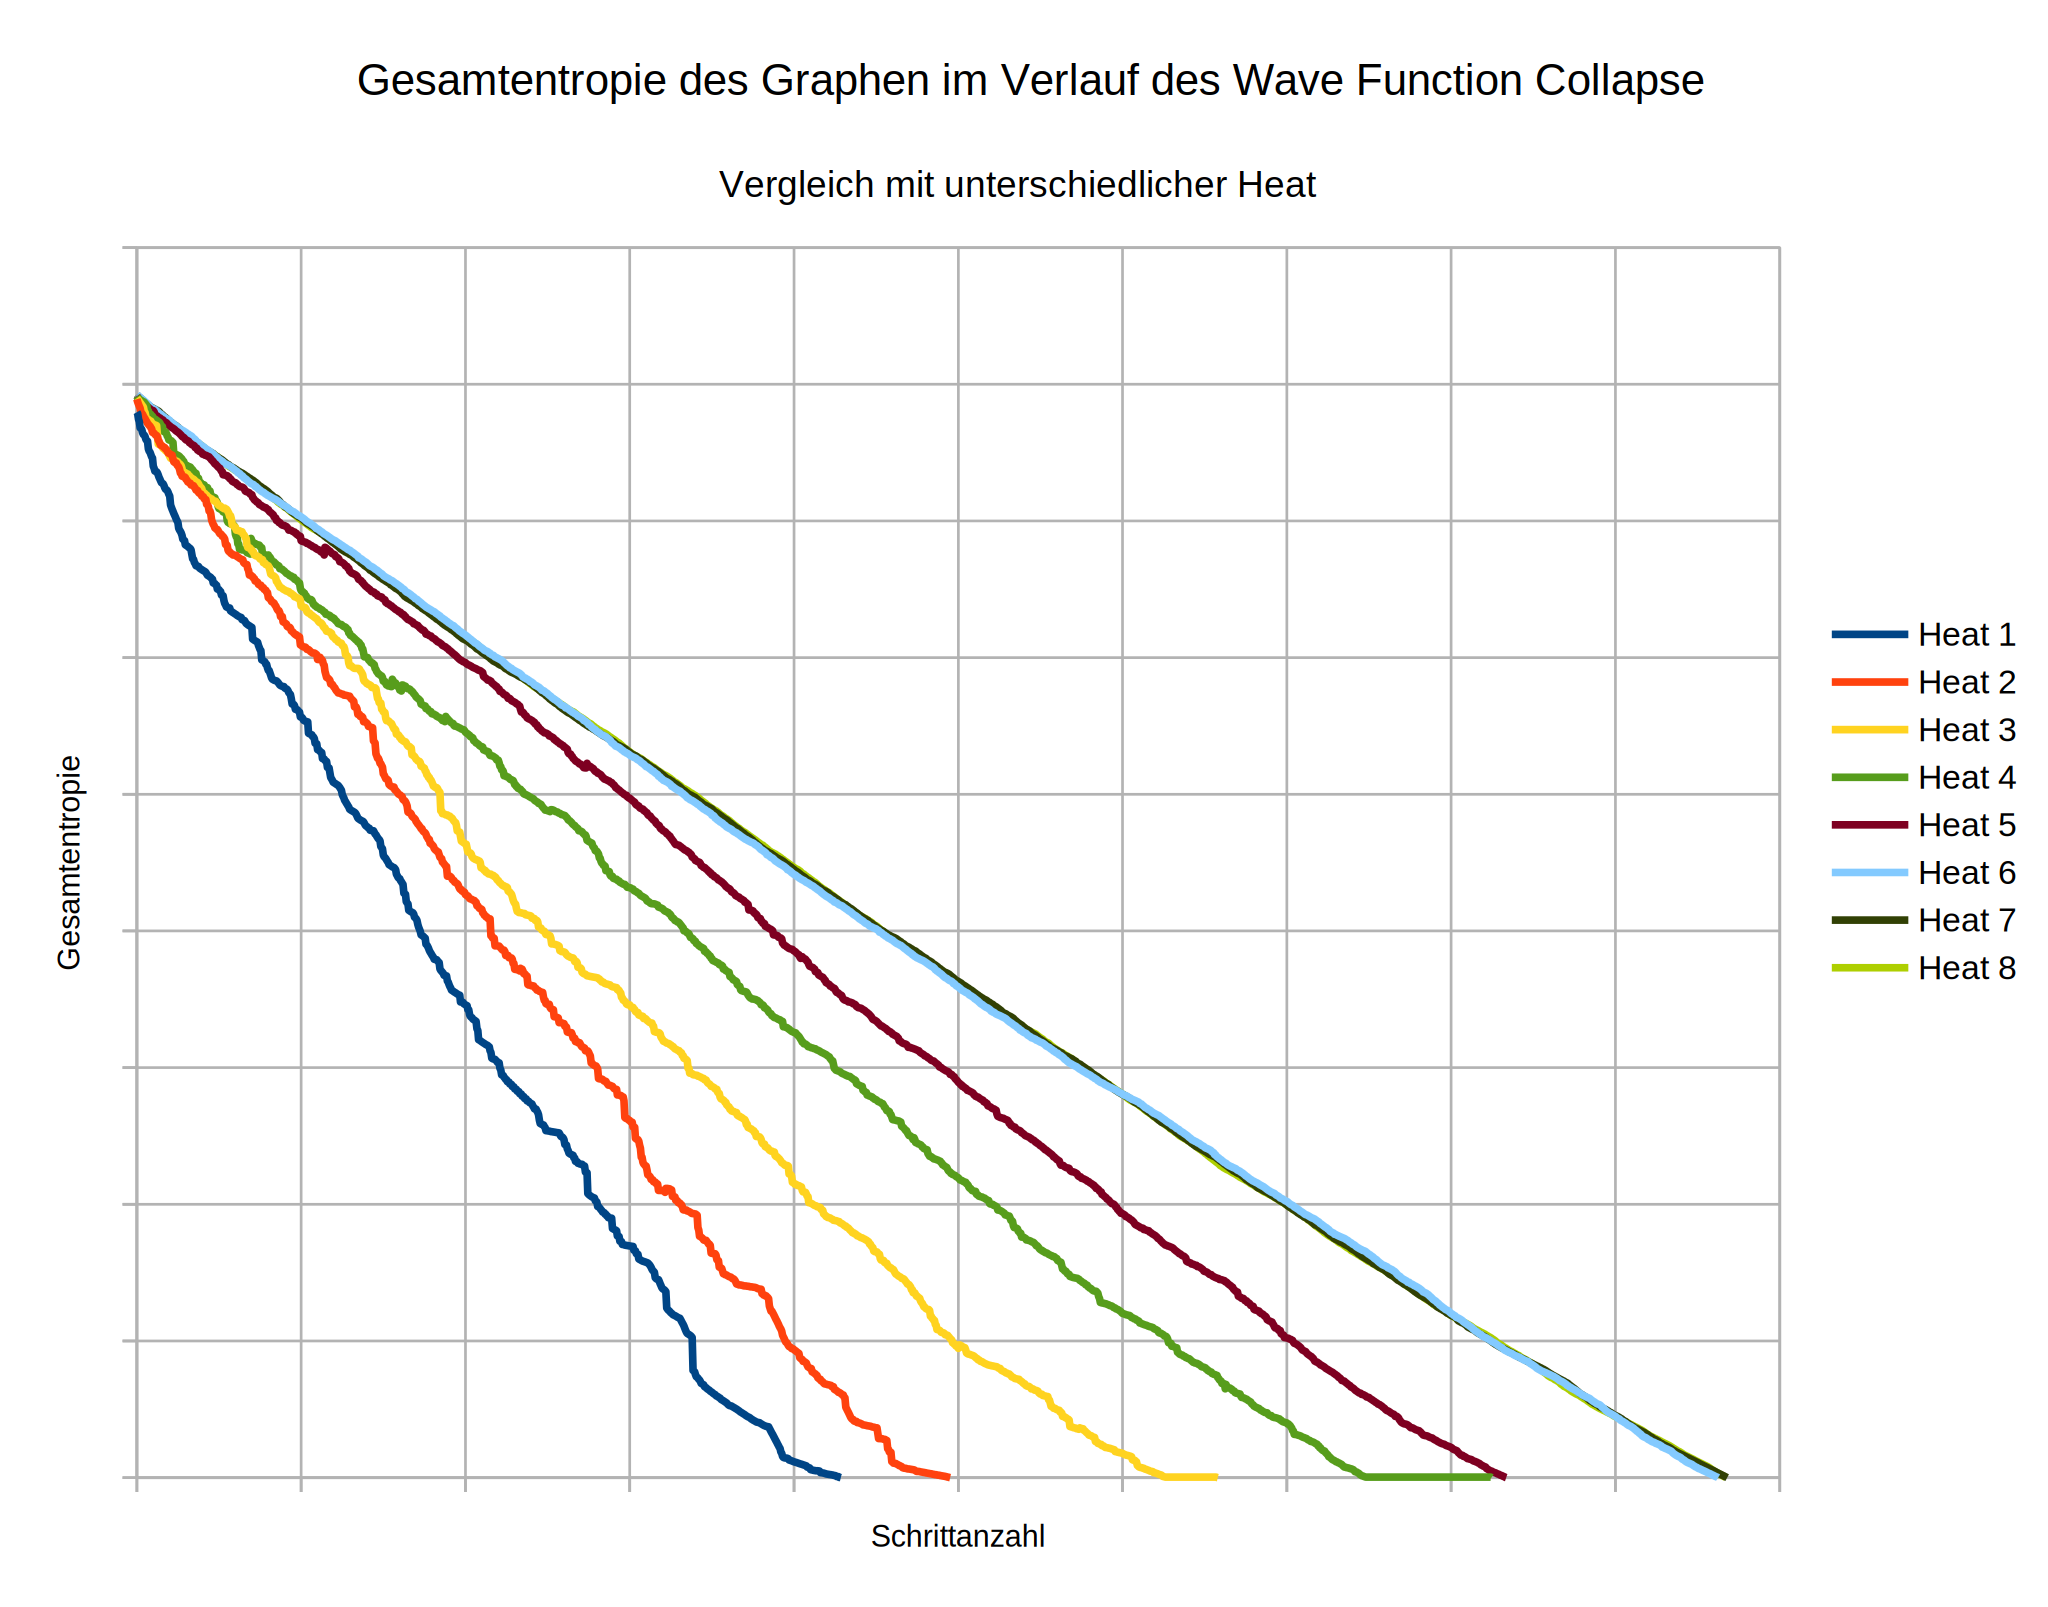
\includegraphics[width=\linewidth]{data/townscaper_grid/1.png} \caption{} \end{subfigure}
    \begin{subfigure}{0.18\textwidth} \includegraphics[width=\linewidth]{data/townscaper_grid/2.png} \caption{} \end{subfigure}
    \begin{subfigure}{0.18\textwidth} \includegraphics[width=\linewidth]{data/townscaper_grid/3.png} \caption{} \end{subfigure}
    \begin{subfigure}{0.18\textwidth} \includegraphics[width=\linewidth]{data/townscaper_grid/4.png} \caption{} \end{subfigure}
    \begin{subfigure}{0.18\textwidth} \includegraphics[width=\linewidth]{data/townscaper_grid/5.png} \caption{} \end{subfigure}
    
    \caption{
        Generierung eines Teils des Gitters für Townscaper \cite{stalberg_grid}. (a) Punkte werden generiert. (b) Triangulierung. (c) Kanten werden gelöscht, so dass Vierecke entstehen. (d) die Vierecke werden geviertelt. (e) Position der Knoten wird aufgelockert, so dass die Winkel zwischen Kanten gleichmäßiger sind.
    }
    \label{fig:townscaper_grid}
\end{figure}
            \pagebreak
            
            Merrel zeigt im Anhang seines Papers \cite{merrel}, dass die Entscheidung, ob eine Ausgabe vervollständigt werden kann, ein NP-vollständiges Problem ist. Einfacher ist es, eine Heuristik zu definieren. Hierfür wird die Shannon-Entropie \cite{shannon} als Maß eingeführt. Sie beschreibt das Maß an Ungewissheit in einem System, hier die Ungewissheit über den finalen Zustand einer Zelle. Sie wird mit der Formel \ref{eq:entropy} berechnet, wobei $\mathcal{X}$ die Menge der möglichen Zustände einer Zelle ist und $p(x)$ die Wahrscheinlichkeit, dass $x$ gewählt wird, ist.
            
            Ist eine Zelle observiert, hat sie nur noch einen Zustand und die Entropie ist 0, während eine Zelle mit vielen Möglichkeiten eine hohe Entropie hat. Die Entropie gibt auch Information darüber, wie sehr eine Zelle durch ihre Umgebung beschränkt wird, da Zellen mit vielen Beschränkungen nur noch wenige mögliche Zustände haben.  
                       
            %     % \caption{
%     %     Formel für die Shannon-Entropie. 
%     %     $\mathcal{X}$ ist die Menge der Möglichen Zustände einer Zelle.
%     %     $p(x)$ ist die Wahrscheinlichkeit das $x$ gewählt wird.
%     % }

\begin{equation}
    \label{eq:entropy}
    \mathrm{entropy}(\mathcal{X}) = -\sum_{x \in \mathcal{X}} p(x),\log p(x)
\end{equation}
        
        
        \subsection{Symmetrie}
            Ziel des Model Synthesis Algorithmus ist es, eine große Anzahl lokal ähnlicher Ausgaben zu generieren \cite{merrel}. Ähnlichkeit wird erreicht, wenn jede kleine Region der Ausgabe zu Regionen des Beispiels passt (siehe Abbildung \ref{fig:wfc_resemblance}). Die wahrgenommene Ähnlichkeit wird verbessert, wenn das Verhältnis der Häufigkeiten von Regionen der Verteilung im Beispiel entspricht. Im Wave Function Collapse wird dieses Kriterium erweitert. Die Regionen können nun auch Drehungen und Spiegelungen der Regionen im Beispiel sein \cite{gumin}.
            
            \begin{figure}[H]
    \centering
    \begin{subfigure}{0.18\textwidth} 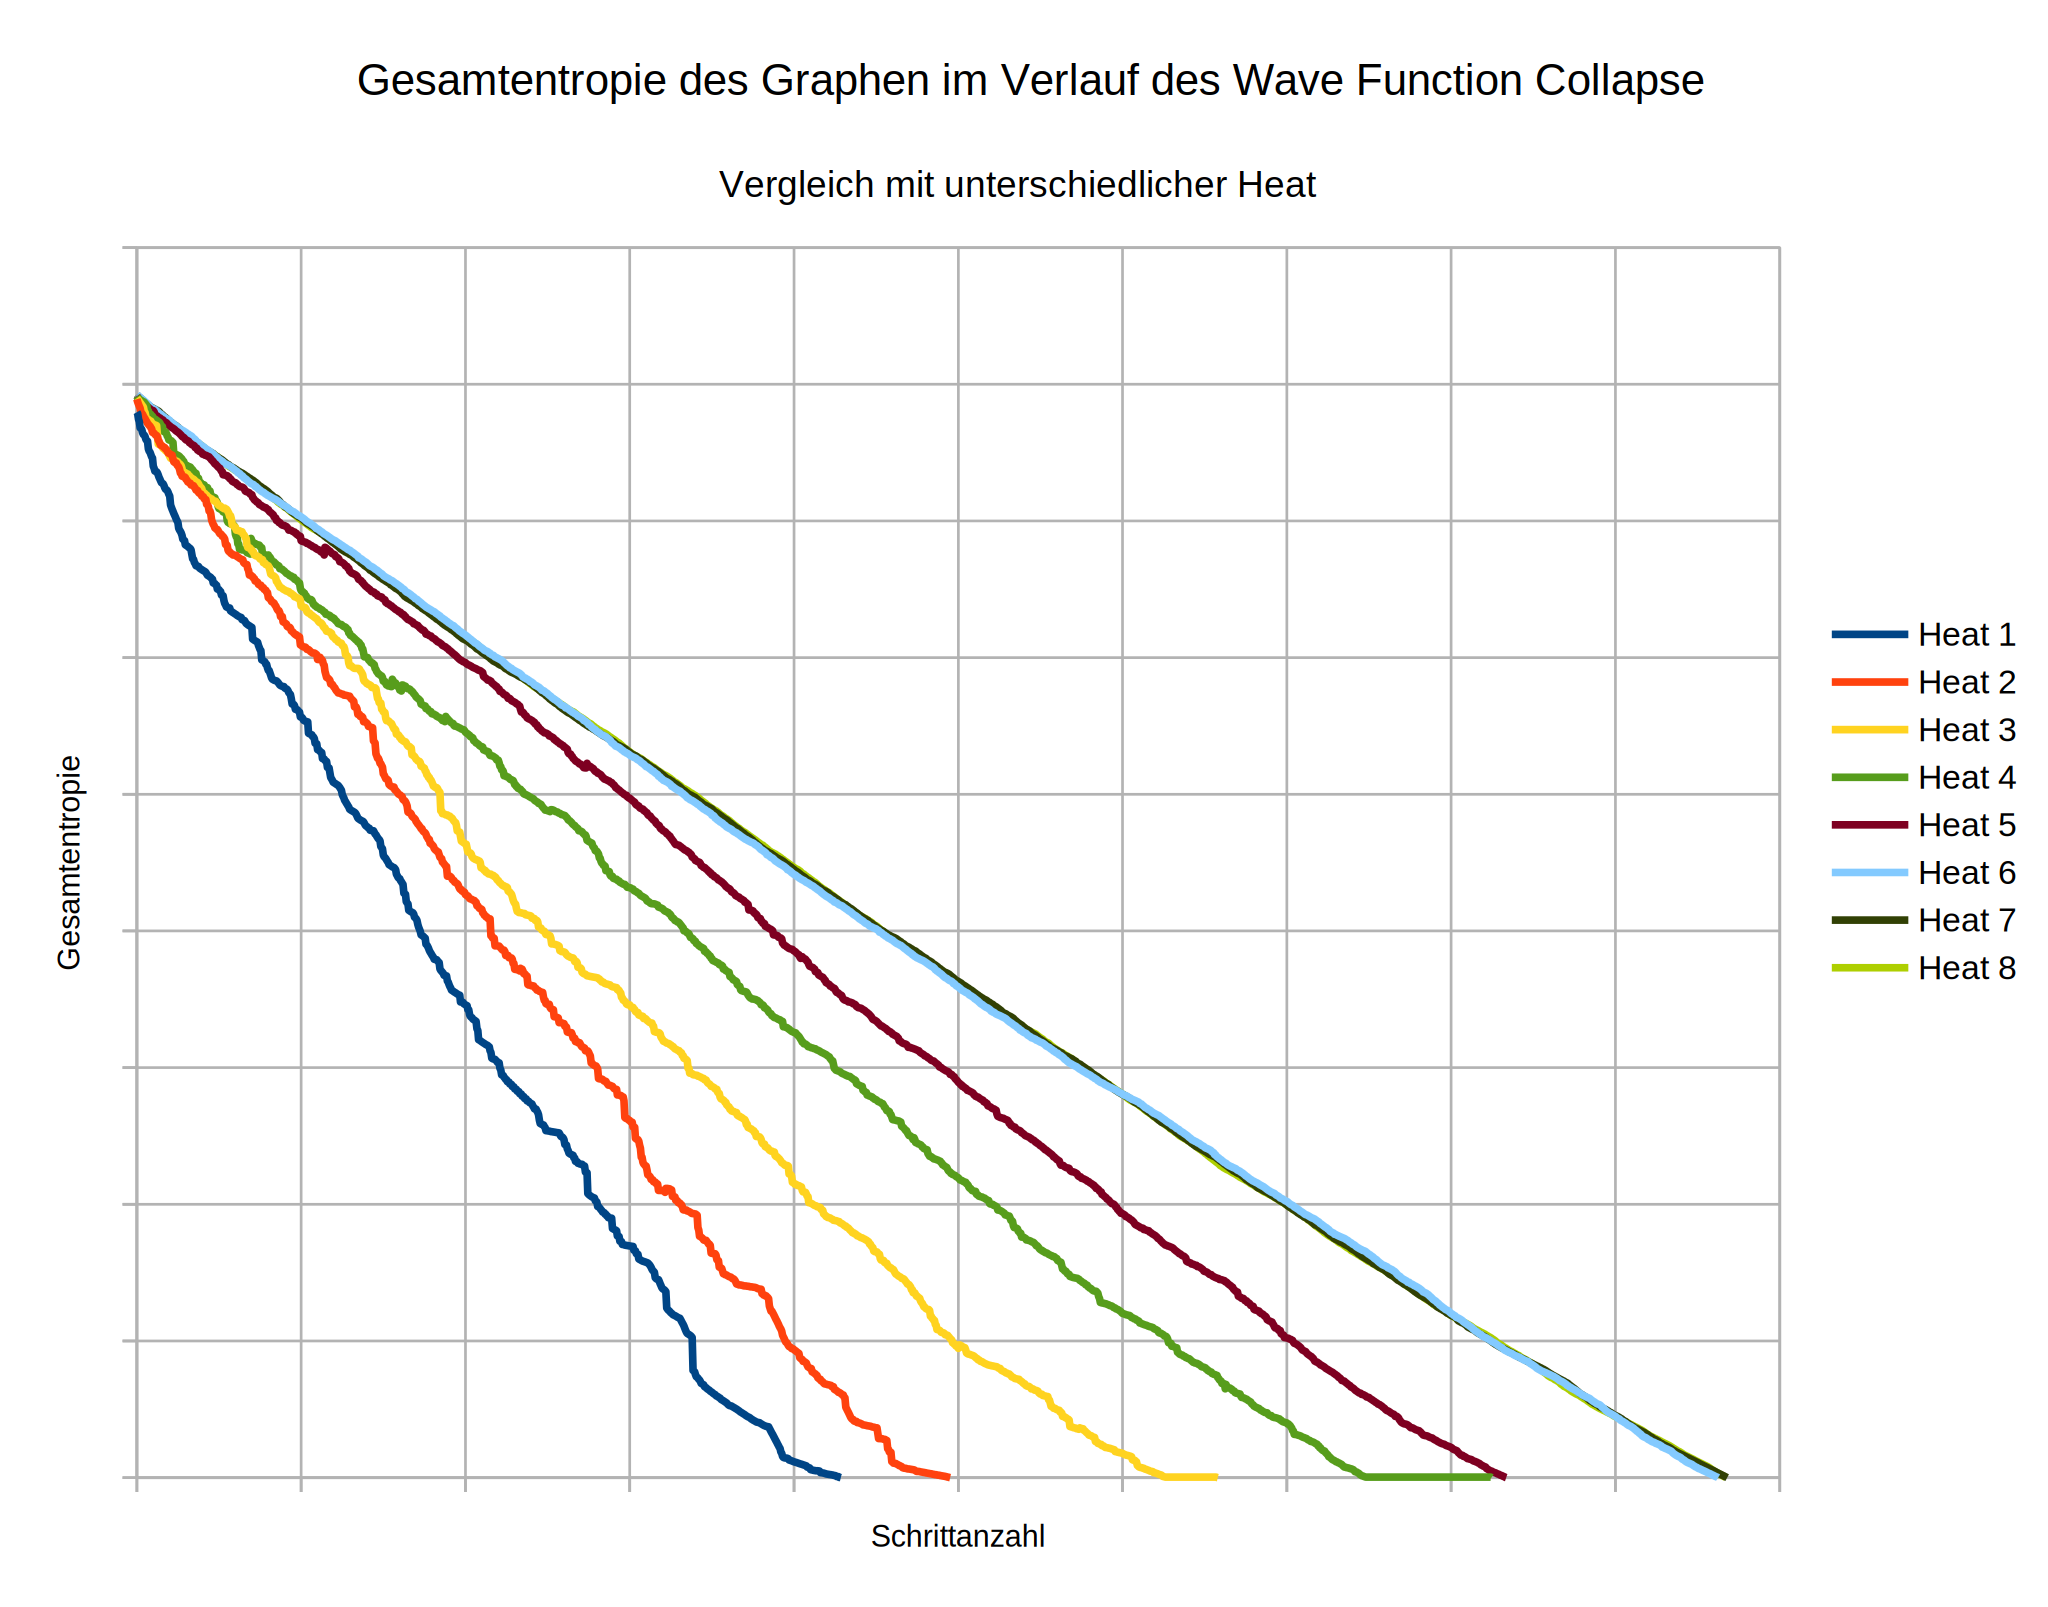
\includegraphics[width=\linewidth]{data/townscaper_grid/1.png} \caption{} \end{subfigure}
    \begin{subfigure}{0.18\textwidth} \includegraphics[width=\linewidth]{data/townscaper_grid/2.png} \caption{} \end{subfigure}
    \begin{subfigure}{0.18\textwidth} \includegraphics[width=\linewidth]{data/townscaper_grid/3.png} \caption{} \end{subfigure}
    \begin{subfigure}{0.18\textwidth} \includegraphics[width=\linewidth]{data/townscaper_grid/4.png} \caption{} \end{subfigure}
    \begin{subfigure}{0.18\textwidth} \includegraphics[width=\linewidth]{data/townscaper_grid/5.png} \caption{} \end{subfigure}
    
    \caption{
        Generierung eines Teils des Gitters für Townscaper \cite{stalberg_grid}. (a) Punkte werden generiert. (b) Triangulierung. (c) Kanten werden gelöscht, so dass Vierecke entstehen. (d) die Vierecke werden geviertelt. (e) Position der Knoten wird aufgelockert, so dass die Winkel zwischen Kanten gleichmäßiger sind.
    }
    \label{fig:townscaper_grid}
\end{figure}
            
            Des weiteren wird eine Annotation für manuell erstellte Bauteile definiert, mit der ein Nutzer einem Bauteil eine Symmetriegruppe zuweisen kann \cite{gumin}. Eine Symmetriegruppe gibt an, wie man ein Bauteil drehen und spiegeln kann. Beim Einlesen generiert der Algorithmus basiert auf dieser Symmetriegruppe weitere, entsprechend gedreht oder gespiegelte, Bauteile, die im weiteren Prozess verwendet werden. Da sich diese Arbeit nicht mit Beispielen aus Bauteilen befasst, sondern primär diese automatisch extrahiert, bleibt dieser Aspekt ungenutzt.
        
        
        \subsection{Extraktion}
            Zuvor musste der Nutzer das gewünschte Beispielmodell oder Beispielbild manuell in einzelne gleichgroße Bauteile zerlegen, aus denen der Algorithmus dann neue Modelle und Bilder generiert. Wave Function Collapse nutzt einen Algorithmus \ref{alg:wfc_extraction} zur Generierung dieser Bauteile \cite{gumin}. Die Größe der Bauteile ist dabei frei wählbar, aber sie sollte so gewählt sein, das sie zum genutzten Beispiel passt, damit die im Beispiel existierenden Muster erhalten bleiben.  Sind die Bauteile zu klein gewählt, gehen Strukturen des Beispiels verloren. Während zu große Bauteile auch unerwünschte Strukturen im Beispiel enthalten, was im extremen Fall dazu führt, dass nur noch exakte Kopien des Beispiels ohne Variation in der Ausgabe vorkommen. Für Bilder wird in dieser Arbeit stets die Moore-Nachbarschaft jedes Pixels, also die direkt angrenzenden Pixel sowie die entlang der Diagonalen, als Bauteil verwendet. Dies wird auch als das Umfeld des Pixels beschrieben.
            
            \begin{algorithm}
    \caption{Regelextraktion}
    \label{alg:wfc_extraction}
    
    \begin{enumerate}
    \item Für jeden Pixel des Beispielbilds:
        \begin{enumerate}
        \item Überschreitet das Umfeld des Pixels den Rand des Bild?
        \subitem Ist Wrapping erlaubt?
        \subsubitem Dann: Nimm die Pixel vom gegenüberliegenden Rand
        \subsubitem Sonst: Überspringe diesen Pixel
        \item Lese das Umfeld aus
        \item Gibt es bereits einen Zustand mit diesem Umfeld?
        \subitem Dann: Erhöhe dessen Frequenz um eins
        \subitem Sonst: Erstelle einen neuen Zustand mit diesem Umfeld
        \end{enumerate}
    
    \item Für jedes Paar Zustände und jede Himmelsrichtung:
        \begin{enumerate}
        \item Prüfe ob die Zustände in dieser Richtung überlappen
        \item Speichere diese Regel in der Lookuptabelle ab
        \end{enumerate}
    \end{enumerate}
        
\end{algorithm}
            
            In Abbildung \ref{fig:extract_wrapping} ist der Ablauf dargestellt. Aus dem Beispiel werden die Umfelder ausgelesen. Dies kann mit oder ohne \textit{Wrapping} passieren, wobei Wrapping bedeutet, dass, wenn z.B. der rechte Rand überschritten wird, es zurück zum linken Rand und von dort aus weitergeht. Dies kann separat für die vertikalen und horizontalen Ränder erlaubt oder verboten werden. Die Zustände ergeben sich aus den einzigartigen Umfeldern. Die Frequenz eines Umfelds gibt an, wie oft es im Beispiel vorkommt. Sind mehrere Umfelder gleich, so hat der entsprechende Zustand eine höhere Frequenz. Aus der Gesamtanzahl an Zuständen und deren Frequenzen lässt sich die Wahrscheinlichkeit jedes Zustands gewählt zu werden berechnen. Im Algorithmus wird dies beachtet, damit die globale Verteilung von Zuständen in der Ausgabe der Verteilung im Beispiel ähnelt. Danach wird geprüft, welche der gefundenen Zustände überlappen. Es werden die Himmelrichtungen N, S, W und O geprüft und für später in einer Lookuptabelle gespeichert.
            
            \begin{figure}[H]
    \centering
    \begin{subfigure}{0.18\textwidth} 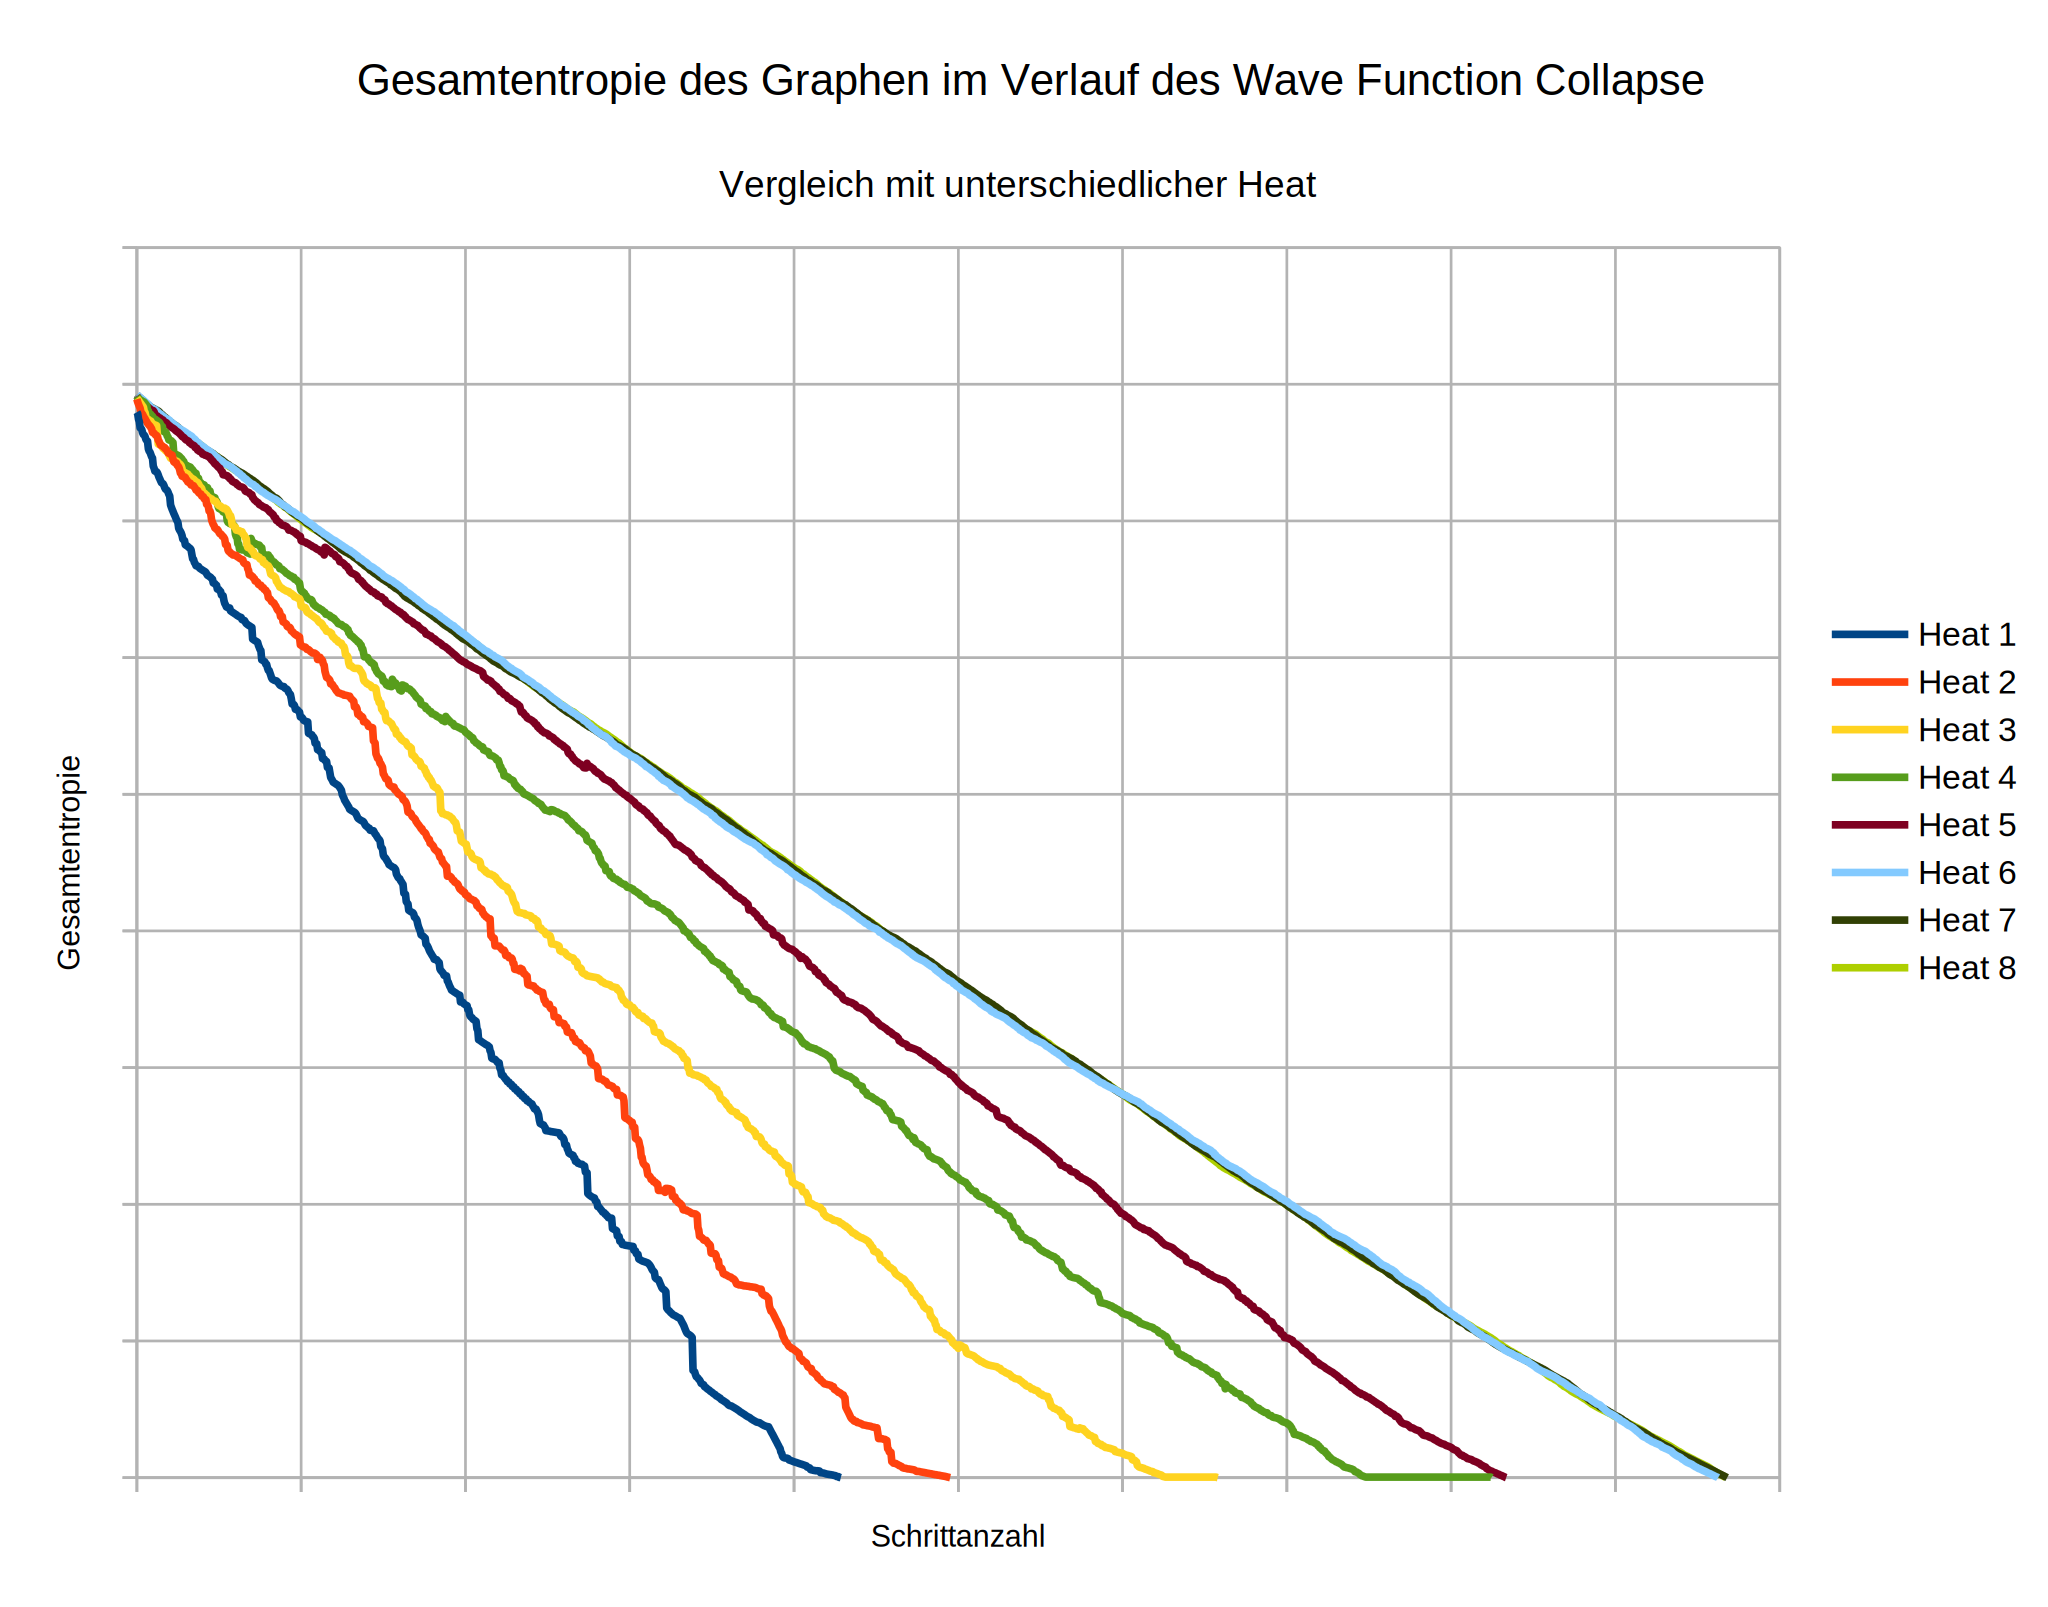
\includegraphics[width=\linewidth]{data/townscaper_grid/1.png} \caption{} \end{subfigure}
    \begin{subfigure}{0.18\textwidth} \includegraphics[width=\linewidth]{data/townscaper_grid/2.png} \caption{} \end{subfigure}
    \begin{subfigure}{0.18\textwidth} \includegraphics[width=\linewidth]{data/townscaper_grid/3.png} \caption{} \end{subfigure}
    \begin{subfigure}{0.18\textwidth} \includegraphics[width=\linewidth]{data/townscaper_grid/4.png} \caption{} \end{subfigure}
    \begin{subfigure}{0.18\textwidth} \includegraphics[width=\linewidth]{data/townscaper_grid/5.png} \caption{} \end{subfigure}
    
    \caption{
        Generierung eines Teils des Gitters für Townscaper \cite{stalberg_grid}. (a) Punkte werden generiert. (b) Triangulierung. (c) Kanten werden gelöscht, so dass Vierecke entstehen. (d) die Vierecke werden geviertelt. (e) Position der Knoten wird aufgelockert, so dass die Winkel zwischen Kanten gleichmäßiger sind.
    }
    \label{fig:townscaper_grid}
\end{figure}

    \section{Visualisierung}
        Die Ausgabe des Wave Function Collapse muss nicht direkt bildlich verwendet werden. Welche Bedeutung die Zellen und deren Zustände haben, ist dem Algorithmus egal. Dieser garantiert nur lokale Ähnlichkeit, zum Beispiel. Im erfolgreichen Spiel \textit{Townscaper} \cite{stalberg_townscaper} von Oskar Stålberg wird Wave Function Collapse verwendet. In Abbildung \ref{fig:townscaper} sind einige Screenshots aus dem Spiel zu sehen.
        
        
        Hier kann die Spielerin aus Gebäuden eine Stadt bauen. Sie wählt dabei aber nicht die konkreten Gebäude aus, sondern legt nur fest, welche Art bzw. Farbe an jeweiliger Stelle platziert werden soll. Das Spiel nutzt Wave Function Collapse, um die dementsprechend am besten passenden Gebäudeteile zu finden. Danach wird das gewählte Modell an den Knotenpunkt angepasst und mit Details wie Fenstern oder Bänken ausgeschmückt.
        
        
        Damit die Stadt nicht geradlinig verläuft, wird sie auf einer spezielle Art von Gitter gebaut. Abbildung \ref{fig:townscaper_grid} zeigt, wie die Teile, aus denen das Gitter besteht, generiert werden. Es ist zu erkennen, dass es auf einer Quadrilierung aufbaut. Eine Quadrilierung ist ein Graph, dessen Kanten Vierecke bilden. Die sechseckigen Regionen werden im Spiel zusammengesetzt und an den Knoten kann die Spielerin Gebäude bauen. Die meisten Knotenpunkte haben vier Kanten, aber es gibt auch einzelne mit drei oder fünf Kanten. Im Spiel existieren für diese Arten von Knoten jeweils unterschiedliche Modelle von Gebäuden. Es müssen keine weiteren Modelle für willkürlich viele Kanten an einem Knoten erstellt werden, da dieser Prozess nur diese drei Arten von Knoten generiert. Es handelt sich also nicht um eine allgemeine Lösung, da die Beispielmodelle speziell für das genutzte Gitter erstellt wurden und nicht für andere Arten von Graphen funktionieren würden.
        
        \begin{figure}[H]
    \centering
    \begin{subfigure}{0.18\textwidth} 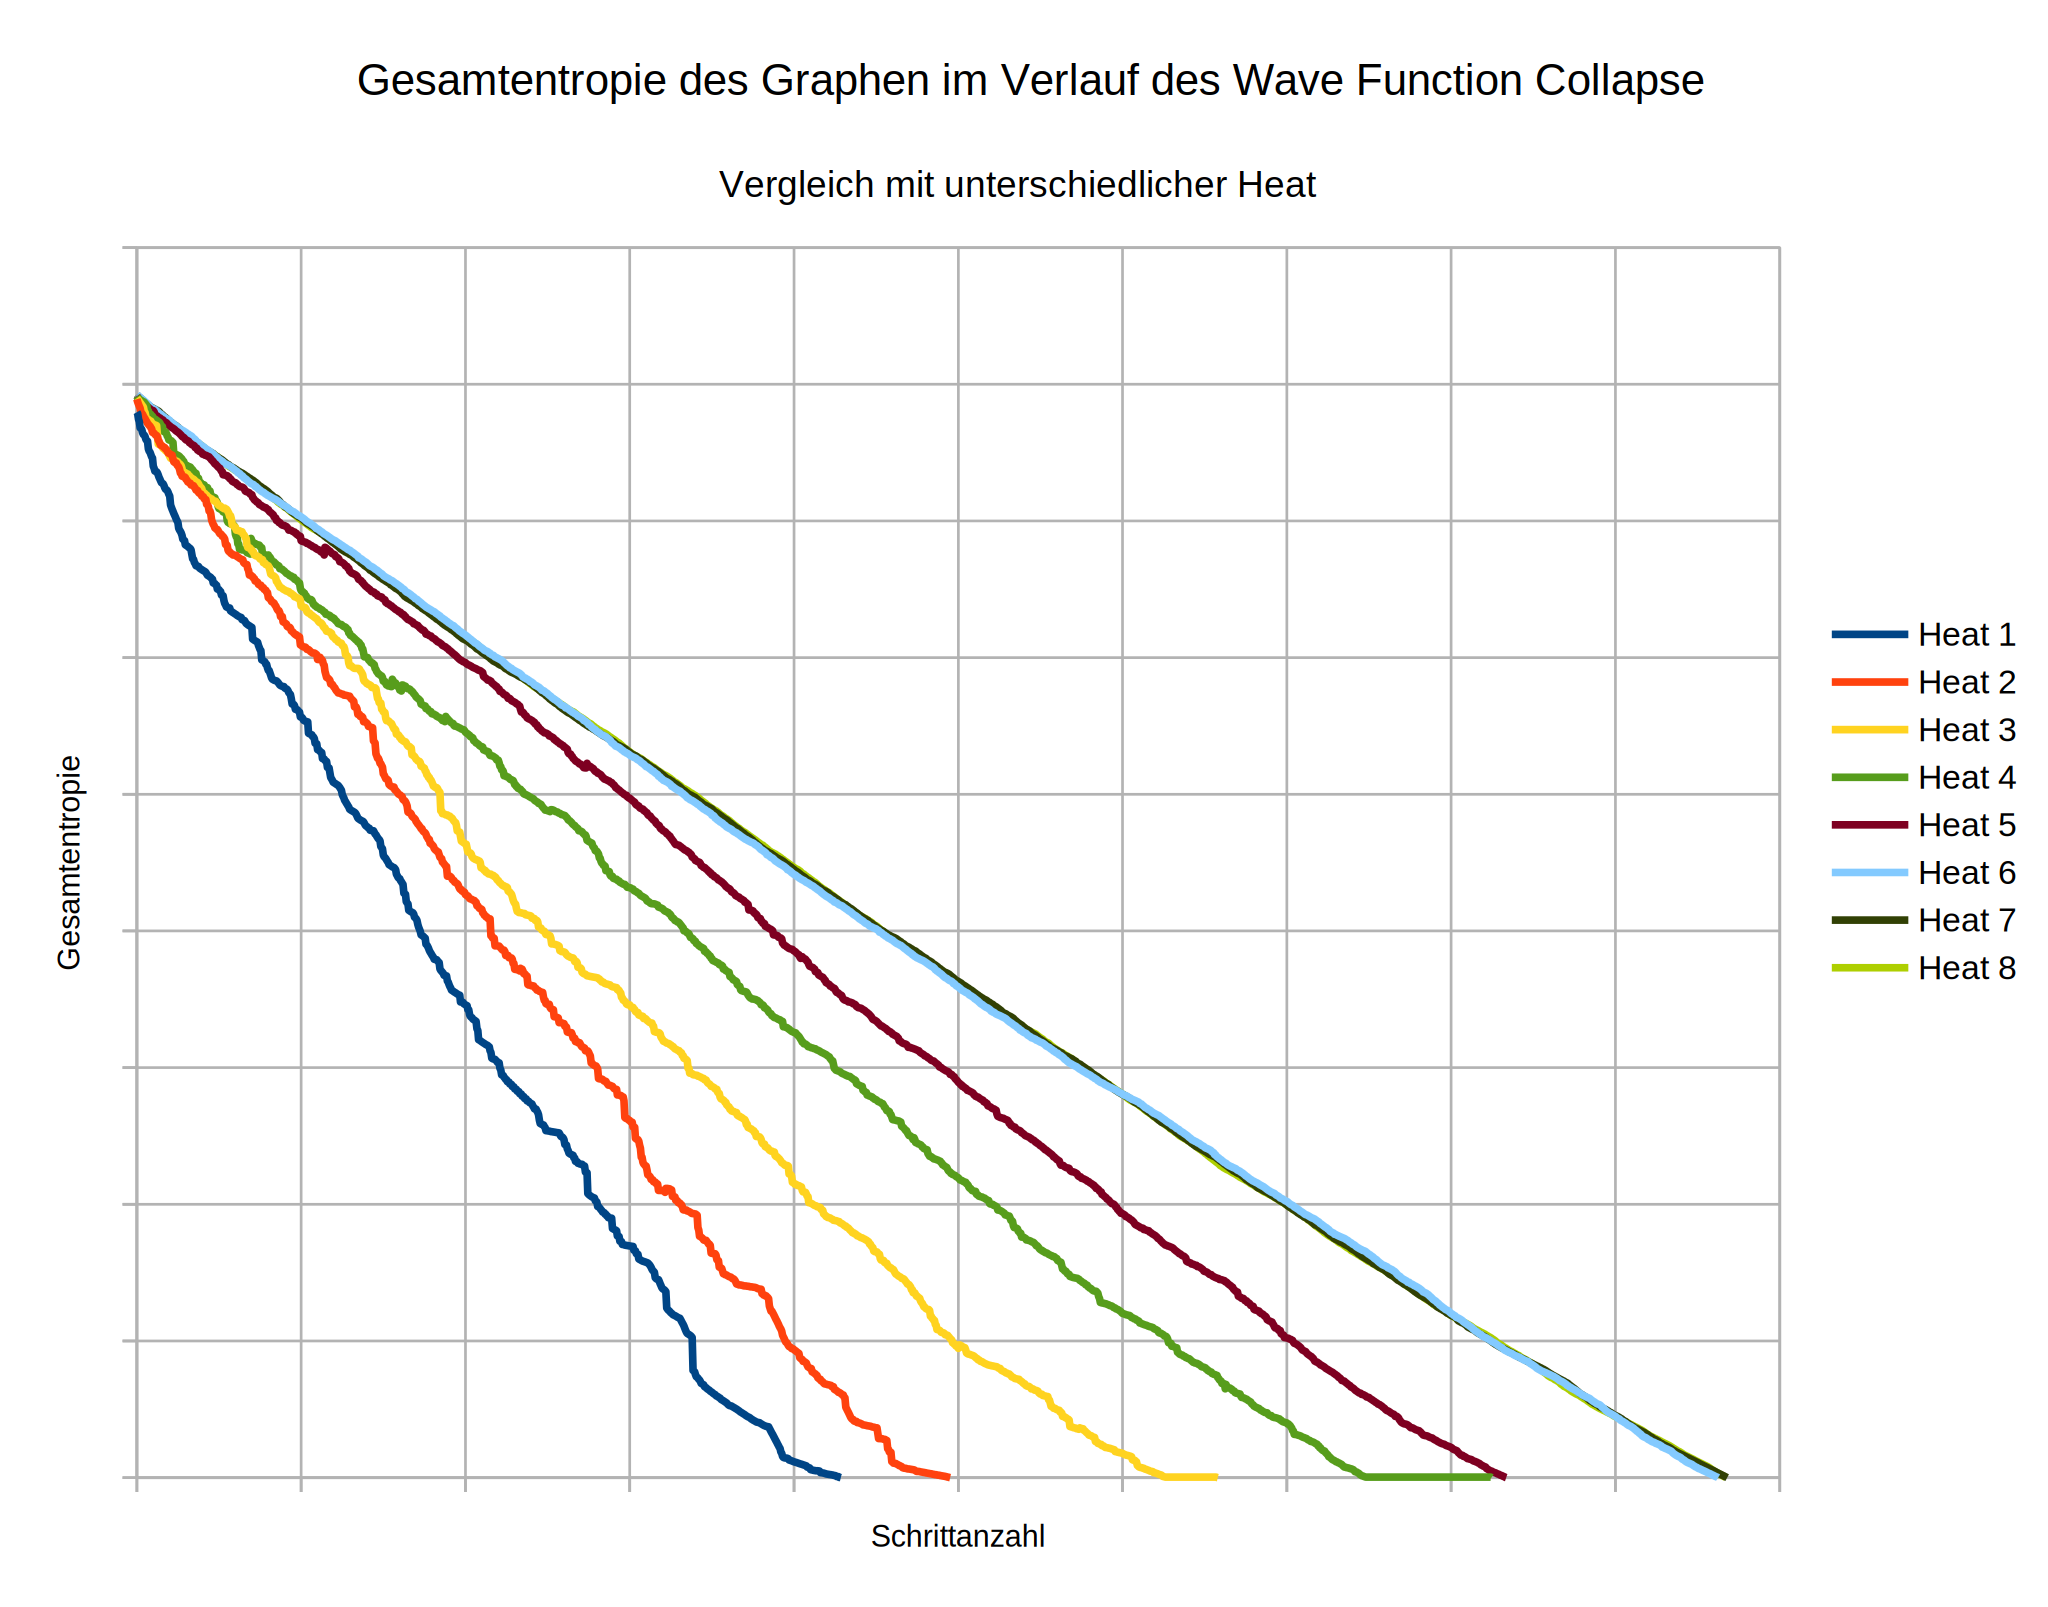
\includegraphics[width=\linewidth]{data/townscaper_grid/1.png} \caption{} \end{subfigure}
    \begin{subfigure}{0.18\textwidth} \includegraphics[width=\linewidth]{data/townscaper_grid/2.png} \caption{} \end{subfigure}
    \begin{subfigure}{0.18\textwidth} \includegraphics[width=\linewidth]{data/townscaper_grid/3.png} \caption{} \end{subfigure}
    \begin{subfigure}{0.18\textwidth} \includegraphics[width=\linewidth]{data/townscaper_grid/4.png} \caption{} \end{subfigure}
    \begin{subfigure}{0.18\textwidth} \includegraphics[width=\linewidth]{data/townscaper_grid/5.png} \caption{} \end{subfigure}
    
    \caption{
        Generierung eines Teils des Gitters für Townscaper \cite{stalberg_grid}. (a) Punkte werden generiert. (b) Triangulierung. (c) Kanten werden gelöscht, so dass Vierecke entstehen. (d) die Vierecke werden geviertelt. (e) Position der Knoten wird aufgelockert, so dass die Winkel zwischen Kanten gleichmäßiger sind.
    }
    \label{fig:townscaper_grid}
\end{figure}
        \begin{figure}[H]
    \centering
    \begin{subfigure}{0.18\textwidth} \includegraphics[width=\linewidth]{data/townscaper_grid/1.png} \caption{} \end{subfigure}
    \begin{subfigure}{0.18\textwidth} \includegraphics[width=\linewidth]{data/townscaper_grid/2.png} \caption{} \end{subfigure}
    \begin{subfigure}{0.18\textwidth} \includegraphics[width=\linewidth]{data/townscaper_grid/3.png} \caption{} \end{subfigure}
    \begin{subfigure}{0.18\textwidth} \includegraphics[width=\linewidth]{data/townscaper_grid/4.png} \caption{} \end{subfigure}
    \begin{subfigure}{0.18\textwidth} \includegraphics[width=\linewidth]{data/townscaper_grid/5.png} \caption{} \end{subfigure}
    
    \caption{
        Generierung eines Teils des Gitters für Townscaper \cite{stalberg_grid}. (a) Punkte werden generiert. (b) Triangulierung. (c) Kanten werden gelöscht, so dass Vierecke entstehen. (d) die Vierecke werden geviertelt. (e) Position der Knoten wird aufgelockert, so dass die Winkel zwischen Kanten gleichmäßiger sind.
    }
    \label{fig:townscaper_grid}
\end{figure}



\chapter{Wave Function Collapse auf Graphen}
    In diesem Kapitel wird dargestellt, wie der Wave Function Collapse Algorithmus erweitert wird, sodass die Ausgabe nicht nur auf einem Gitter, sondern auch auf Zellen mit freier Anordnung und Verteilung, einem Graphen, erfolgen kann. Es wird erklärt, welche Aspekte des Algorithmus angepasst werden. Des weiteren wird ein neues Konzept namens \textit{Heat} eingeführt, womit die Erfolgsquote des Algorithmus für spezielle Graphen verbessert wird, indem Überlappungsregeln abgeschwächt werden, wodurch die Ausgabe eine geringere Ähnlichkeit zum Beispiel haben kann.
    
    
    \section{Beschränkung des Algorithmus und Idee zur Erweiterung}
        Die ursprüngliche Form des Wave Function Collapse nimmt ein 2D Pixelmuster oder Tilesets als Beispiel und produziert daraus wieder 2D Muster. Pixel liegen stets auf einem Gitter. Bei Tilesets ist die grafische Gestaltung des Tiles zwar uneingeschränkt, dennoch sind die Tiles selbst quadratisch. Dies schränkt die Gestaltung des Inhalts der Tiles insofern ein, dass die Kanten zu anderen Kanten passen müssen. Auch bei 3D Beispielen werden die Modelle in blockförmige Bauteile zerschnitten, damit der Algorithmus auf einem 3D Gitter von Würfeln arbeiten kann.
        
        Gitter bringen bestimmte Vorteile durch ihre Struktur mit sich. Die Benachbarung von Zellen ist implizit aus dem Gitter erkennbar, die Nachbarzellen befinden sich stets in festen Abständen in die vier Himmelsrichtungen im 2D Gitter und entlang der drei Achsen, also 6 Richtungen, im 3D Gitter. Die Überlappungsregeln aus dem Beispiel können also direkt von einem Gitter auf das andere übertragen werden. Der Nachteil solcher Gitter ist, dass die Ausgabe im Ganzen Artefakte des Gitters aufweist (siehe Abbildung \ref{fig:aliasing}). Nur vertikale und horizontale Linien können im Pixelgitter exakt dargestellt werden, frei geformte Kurven oder organische Strukturen lassen sich nur durch Annäherung darstellen und es kann zu Aliasing kommen.
        
        \begin{figure}[H]
    \centering
    \begin{subfigure}{0.18\textwidth} \includegraphics[width=\linewidth]{data/townscaper_grid/1.png} \caption{} \end{subfigure}
    \begin{subfigure}{0.18\textwidth} \includegraphics[width=\linewidth]{data/townscaper_grid/2.png} \caption{} \end{subfigure}
    \begin{subfigure}{0.18\textwidth} \includegraphics[width=\linewidth]{data/townscaper_grid/3.png} \caption{} \end{subfigure}
    \begin{subfigure}{0.18\textwidth} \includegraphics[width=\linewidth]{data/townscaper_grid/4.png} \caption{} \end{subfigure}
    \begin{subfigure}{0.18\textwidth} \includegraphics[width=\linewidth]{data/townscaper_grid/5.png} \caption{} \end{subfigure}
    
    \caption{
        Generierung eines Teils des Gitters für Townscaper \cite{stalberg_grid}. (a) Punkte werden generiert. (b) Triangulierung. (c) Kanten werden gelöscht, so dass Vierecke entstehen. (d) die Vierecke werden geviertelt. (e) Position der Knoten wird aufgelockert, so dass die Winkel zwischen Kanten gleichmäßiger sind.
    }
    \label{fig:townscaper_grid}
\end{figure}
        
        Im Kern des Wave Function Collapse wird geprüft, dass nur Zustände gewählt werden, die mit der Ausgabe bis dahin überlappen könnten. Die möglichen Überlappungen hängen dabei von der Richtung zwischen den Zellen ab. In einem Gitter kann jede Richtung zu einer Nachbarzelle aus dem Beispiel extrahiert werden. Wird die Anordnung und Benachbarung der Zellen nun aber vom Gitter gelöst, so ist es nicht mehr garantiert, dass die Richtungen zwischen Nachbarzellen auch im Beispiel existieren. Stattdessen müssen die tatsächlichen Richtungen auf eine der extrahierbaren Richtungen übersetzt werden. Danach kann der Algorithmus wie zuvor mit den Überlappungsregeln arbeiten, um nun den Graphen zu befüllen.
    
    
    \section{Von Gittern zu Graphen}
        Ursprünglich arbeitet Wave Function Collapse nur auf Gittern \cite{merrel, gumin}. Der Schritt zum Graphen als Fundament für die Ausgabe des Algorithmus ist naheliegend, da Gitter eine spezielle Art von Graphen darstellen. Im Umfang dieser Arbeit werden jedoch nicht alle Arten von Graphen betrachtet. Da jede Kante eines Gitters zuvor eine lokale Benachbarung dargestellt hat und die Regelextraktion nur lokal arbeitet, beschränkt sich diese Arbeit nur auf Graphen, in denen Kanten primär einen Knotenpunkt mit den Knotenpunkten in einem lokalen Bereich verbindet. Der Algorithmus kann auch auf anderen Arten von Graphen angewendet werden, doch können daraus neue oder unerwartete Effekte hervortreten, die wiederum andere Lösungswege benötigen.
        
        Ein Gitter enthält implizit Informationen über Benachbarung und Position jeder Zelle. Diese Informationen werden bei Graphen explizit angegeben. Dazu kommt, dass je nach Anordnung nun nicht nur die Richtung zur Nachbarzelle, sondern auch deren Abstand und die Anzahl der Nachbarzellen variieren kann. Dieser Aspekt ist von Vorteil für die Gestaltung der Ausgabe, da nun beliebige Strukturen und Formen genutzt werden können. Doch der Nachteil ist, dass das Beispiel und die daraus extrahierten Regeln vom Algorithmus nicht mehr eins zu eins angewendet werden können.
        
        
        
    \section{Heat}
        In einem 2D Gitter sind die Nachbarn jeder Zelle per Definition in festen Richtungen und Abständen zu finden. Bei Graphen ist diese Anordnung frei. Während des Algorithmus werden die möglichen Zustände von Nachbarzellen auf Überlappung geprüft. Ein Zustand einer Zelle ist möglich, wenn er mit mindestens einem Zustand jeder Nachbarzelle überlappen kann. Die Überlappung zweier Zustände hängt von der Richtung zwischen den Umfeldern der Zustände ab. Das heißt, dass für den Nachbarn im Norden einer Zelle nur die Überlappung der Zustände im Norden relevant ist. Die Richtung zu einer Nachbarzelle in einem Graphen wird als der Vektor vom Mittelpunkt der Zelle zum Mittelpunkt der Nachbarzelle definiert. Der wichtigste Unterschied ist, dass die Richtung nun nicht mehr, wie im Gitter, auf die Himmelsrichtungen beschränkt ist. 
        
        Es ist nicht möglich, Regeln für eine beliebige Richtung aus dem Beispiel zu extrahieren, da jeder Pixel nur 8 angrenzende Pixel hat. Sieht man das Beispiel als eine Funktion an, so ist diese nicht an allen Punkten definiert. Man könnte durch Interpolation einen Mittelwert zwischen Pixeln berechnen, wenn das Bild eine kontinuierliche Funktion approximiert. Handelt es sich aber tatsächlich um eine diskrete Funktion, könnte eine Interpolation Werte ergeben, die nicht Teil des Wertebereichs waren; in anderen Worten würde man Farbwerte erhalten, die vorher nicht im Bild waren. Da die Ausgabe dem Beispiel ähnlich sein muss, entfällt diese Option.
        
        Es bleibt also nur die Möglichkeit, dass der tatsächlichen Richtung eine der messbaren Himmelsrichtungen zugewiesen wird. Hierfür wird die Kosinus-Ähnlichkeit berechnet (siehe Formel \ref{eq:cosine}). Ist der Wert hoch, so zeigen die Vektoren in eine ähnliche Richtung, während entgegengesetzte Vektoren eine geringe Ähnlichkeit haben. Es wird die Himmelsrichtung mit der höchsten Ähnlichkeit gewählt. 
        
        \begin{figure}[H]
    \centering
    
    $$ \mathrm{similarity}(\mathbf{a},\mathbf{b}) = \frac{\mathbf{a}\cdot\mathbf{b}}{\|\mathbf{a}\|_2\,\|\mathbf{b}\|_2} $$
    
    \caption{Formel für die Kosinus-Ähnlichkeit}
    
    \label{fig:cosine}
\end{figure}
        
        Nun kann mit dieser Auswahl weitergearbeitet werden. Der Nachbar wird als in dieser Himmelrichtung liegend behandelt und daraus ergibt sich, welche Überlappungsregeln benutzt werden. Sind die Zellen beinahe oder ausschließlich entlang der Himmelrichtungen angeordnet, funktioniert diese Rundung gut. Liegt eine Nachbarrichtung nun aber genau zwischen zwei Himmelrichtungen, so haben beide die gleiche Ähnlichkeit und der Algorithmus muss willkürlich eine der beiden wählen. Diese Entscheidung wird bereits vor Beginn der Generierung getroffen, was den schlechtesten Zeitpunkt dafür darstellt, da am wenigsten Informationen vorliegen. Um zu wissen, welche Himmelrichtung bessere Ergebnisse liefert, müssten beide Optionen jeweils ausprobiert und verglichen werden. Da jede Zelle mit ihrem finalen Zustand aber jede andere Zelle beeinflussen kann, müsste jede Kombination für alle Zellen geprüft werden, was schnell unmöglich wird. Stattdessen wäre es besser, die Entscheidung bis zum letzten Moment, also dann, wenn eine Zelle kollabiert, aufzuschieben. Zu diesem Zeitpunkt hat der Algorithmus die meisten Informationen und kann dadurch einen Widerspruch besser vermeiden. Beim Kollabieren wird der Zelle immer noch ein einziger Zustand zugewiesen, wodurch implizit die Himmelsrichtung ausgewählt wird, mit der der gewählte Zustand mit den Nachbarzellen überlappt.
        \\
        \\
        \pagebreak
        \textit{Heat} gibt an, wie viele Himmelrichtungen der Algorithmus für Nachbarn betrachtet. Diese wird im Umfang dieser Arbeit für alle Zellen des Graphen einheitlich gesetzt und vor Beginn der Generierung festgelegt. Damit ein Zustand nun für eine Zelle möglich ist, muss dieser mit den Zuständen der Nachbarzellen überlappen. Nun muss die Überlappung entsprechend der Heat nicht nur entlang einer Himmelrichtung sein, sondern es können mehrere geprüft werden, wobei es reicht, wenn eine der Himmelsrichtungen eine passende Regel hat. Ein Effekt höherer Heat ist, dass Zellen mehr mögliche Zustände haben, da es für jeden Zustand mehr passende Regeln gibt; die Entropie der Zellen ist tendenziell höher als bei geringer Heat.
        
        Die Anzahl der extrahierten Himmelsrichtungen begrenzt den Wertebereich für die Heat. Jeder Benachbarung kann minimal eine und maximal alle Himmelsrichtungen zugewiesen werden. Da Wave Function Collapse zuvor auf Gittern lief, konnte die Regelextraktion optimiert werden. Die reguläre Struktur des Gitters führt dazu, dass, wenn für eine Zelle $A$ der Nachbar von $A$ im Norden($A_n$) passt und der Nachbar im Westen von $A_n$ passt, dann muss auch der Nachbar von $A$ im Nordwesten passen. Somit mussten nur die Überlappungsregeln für Norden, Süden, Westen und Osten gespeichert werden. Für die Generierung auf Graphen entfällt dies. Die diagonalen Himmelsrichtungen werden explizit gespeichert und behandelt.
    
    
    
    \section{Zusammenfassung}
        Ziel dieser Arbeit ist es, die Generierung des Wave Function Collapse Algorithmus auf Graphen geschehen zu lassen. Hierfür wurden drei Anpassungen dargestellt:
        \begin{enumerate}
            \item Ein Gitter gibt implizit an, wo Zellen liegen und welche Zellen benachbart sind. Diese Informationen müssen im Graphen explizit gespeichert werden. 
            \item Für Gitter genügt es bei der Regelextraktion die Himmelrichtungen entlang der Achsen zu betrachtet. Bei Graphen sollten aber auch die Diagonalen extrahiert und gespeichert werden.
            \item Die aus dem Beispiel extrahierten Überlappungsregeln können nicht wie bei Gittern direkt angewendet werden. Die für eine Nachbarzelle relevanten Regeln werden aus der tatsächlichen Richtung zu dieser berechnet. Diese Zuweisung wird mittels Heat erweitert, sodass mehr als eine Himmelsrichtung ausgewählt werden kann.
        \end{enumerate} 



\chapter{Umsetzung}
    Abbildung \ref{fig:app} zeigt einen Screenshot der für diese Arbeit entwickelten Anwendung, in dem die Benutzeroberfläche und eine generierte Ausgabe zu sehen sind. Der Nutzer kann Beispielbilder auswählen, einen Graphen generieren und dann mittels Wave Function Collapse eine Ausgabe generieren. Der Quellcode ist hier\footnote{\url{https://github.com/MrMetube/wfc} (Stand: \today)} verfügbar.
    
    \begin{figure}[H]
    \centering
    \begin{subfigure}{0.18\textwidth} \includegraphics[width=\linewidth]{data/townscaper_grid/1.png} \caption{} \end{subfigure}
    \begin{subfigure}{0.18\textwidth} \includegraphics[width=\linewidth]{data/townscaper_grid/2.png} \caption{} \end{subfigure}
    \begin{subfigure}{0.18\textwidth} \includegraphics[width=\linewidth]{data/townscaper_grid/3.png} \caption{} \end{subfigure}
    \begin{subfigure}{0.18\textwidth} \includegraphics[width=\linewidth]{data/townscaper_grid/4.png} \caption{} \end{subfigure}
    \begin{subfigure}{0.18\textwidth} \includegraphics[width=\linewidth]{data/townscaper_grid/5.png} \caption{} \end{subfigure}
    
    \caption{
        Generierung eines Teils des Gitters für Townscaper \cite{stalberg_grid}. (a) Punkte werden generiert. (b) Triangulierung. (c) Kanten werden gelöscht, so dass Vierecke entstehen. (d) die Vierecke werden geviertelt. (e) Position der Knoten wird aufgelockert, so dass die Winkel zwischen Kanten gleichmäßiger sind.
    }
    \label{fig:townscaper_grid}
\end{figure}
    
    \section{Generierung von Graphen}
        Die Graphen, auf denen der Wave Function Collapse arbeiten soll, werden in dieser Arbeit mit Algorithmus \ref{alg:graph_gen} generiert. Der Algorithmus nimmt als Eingabe eine Menge an Punkten, die die Knotenpunkte des Graphen werden. Aus den Punkten wird eine Delaunay-Triangulierung erstellt. Hierfür wird der Boywer-Watson \cite{bowyer, watson} Algorithmus verwendet (siehe Algorithmus \ref{alg:bowyer_watson}). Danach wird das Voronoi-Diagramm zur Triangulierung gefunden. Der duale Graph der Delaunay-Triangulierung ist das Voronoi-Diagramm, d.h. jeder Knotenpunkt des Voronoi-Diagramms entspricht einer Fläche der Triangulierung und jede Fläche im Voronoi-Diagramm entspricht einem Knotenpunkt in der Triangulierung. Die Kanten der Dreiecke geben an, welche Zellen aneinander angrenzen, während die Voronoi-Zellen die Form einer Zelle für die Darstellung geben. In Abbildung \ref{fig:graph_examples} sind einige Beispiele von generierten Graphen dargestellt. Es ist zu erkennen, dass regelmäßige Gitter nur eine spezielle Form von Graphen darstellen. Daher können regelmäßige Gitter und unregelmäßige Graphen in einem Graphen kombiniert werden.
        
        \begin{algorithm}
    \caption{Generierung eines Graphen}
    \label{alg:graph_gen}
        
    \begin{enumerate}
    \item Erstelle eine Menge an Punkten
    
    \item Generiere die Delaunay-Triangulierung der Punkte
    \subitem Die Ecken und Kanten aller Dreiecke bilden den Graphen
        
    \item Erstelle die Voronoi-Zellen aus der Triangulierung \begin{enumerate}
        \item Finde alle Dreiecke, die einen Punkt teilen
        \item Die Schwerpunkte dieser Dreiecke sind die Eckpunkte der Zelle
        \item Verbinde die Eckpunkte der Zelle mit Kanten
        \item Begrenze die Voronoi-Zellen auf den gewünschten Bereich 
        \subitem siehe Abbildung \ref{fig:voronoi_clipping}
        \end{enumerate}
    \end{enumerate}
        
\end{algorithm}
        
        \begin{algorithm}
    \caption{Bowyer-Watson Algorithmus \cite{bowyer, watson}}
    \label{alg:bowyer_watson}
        
    \begin{enumerate}
        \item Geben sei eine Menge an Punkte
        \item Erstelle das Super-Dreieck so dass jeder Punkt innerhalb liegt
        
        \item Füge jeden Punkt schrittweise in die Triangulierung ein: \begin{enumerate}
            \item Finde die Dreiecke in dessen Umkreis der Punkt liegt
            \subitem Ist der Punkt innerhalb des Umkreises kann dieses Dreieck nicht zur finalen Triangulierung gehören
            \item Sammel alle Kanten dieser Dreiecke
            \subitem Kommt eine Kante nur einmal vor, ist sie Teil der Hülle dieser Dreiecke
            \subitem Alle anderen Kanten sind innerhalb dieser Hülle, da sich zwei Dreiecke diese Kante teilen
            \item Erstelle eine neue Kante zum eingefügten Punkt für jede Ecke der Hülle
            \item Erstelle neue Dreiecke aus diesen Kanten und der Hülle
            \item Füge die neuen Dreiecke in die Triangulierung ein
        \end{enumerate}
        
        \item Enferne alle Dreiecke die eine Kanten mit dem Super-Dreieck teilen
        \item Die Ecken und Kanten aller Dreiecke bilden den Graphen
        \subitem Jede Ecke wird der Mittelpunkt einer Voronoi-Zelle
        \subitem Die Kanten zeigen welche Zellen benachbart sind
    \end{enumerate}
        
\end{algorithm}
        
        \pagebreak
        
        \begin{figure}[H]
    \centering
    \begin{subfigure}{0.18\textwidth} \includegraphics[width=\linewidth]{data/townscaper_grid/1.png} \caption{} \end{subfigure}
    \begin{subfigure}{0.18\textwidth} \includegraphics[width=\linewidth]{data/townscaper_grid/2.png} \caption{} \end{subfigure}
    \begin{subfigure}{0.18\textwidth} \includegraphics[width=\linewidth]{data/townscaper_grid/3.png} \caption{} \end{subfigure}
    \begin{subfigure}{0.18\textwidth} \includegraphics[width=\linewidth]{data/townscaper_grid/4.png} \caption{} \end{subfigure}
    \begin{subfigure}{0.18\textwidth} \includegraphics[width=\linewidth]{data/townscaper_grid/5.png} \caption{} \end{subfigure}
    
    \caption{
        Generierung eines Teils des Gitters für Townscaper \cite{stalberg_grid}. (a) Punkte werden generiert. (b) Triangulierung. (c) Kanten werden gelöscht, so dass Vierecke entstehen. (d) die Vierecke werden geviertelt. (e) Position der Knoten wird aufgelockert, so dass die Winkel zwischen Kanten gleichmäßiger sind.
    }
    \label{fig:townscaper_grid}
\end{figure}
        
        \pagebreak
        
        \begin{figure}[H]
    \centering
    \begin{subfigure}{0.18\textwidth} \includegraphics[width=\linewidth]{data/townscaper_grid/1.png} \caption{} \end{subfigure}
    \begin{subfigure}{0.18\textwidth} \includegraphics[width=\linewidth]{data/townscaper_grid/2.png} \caption{} \end{subfigure}
    \begin{subfigure}{0.18\textwidth} \includegraphics[width=\linewidth]{data/townscaper_grid/3.png} \caption{} \end{subfigure}
    \begin{subfigure}{0.18\textwidth} \includegraphics[width=\linewidth]{data/townscaper_grid/4.png} \caption{} \end{subfigure}
    \begin{subfigure}{0.18\textwidth} \includegraphics[width=\linewidth]{data/townscaper_grid/5.png} \caption{} \end{subfigure}
    
    \caption{
        Generierung eines Teils des Gitters für Townscaper \cite{stalberg_grid}. (a) Punkte werden generiert. (b) Triangulierung. (c) Kanten werden gelöscht, so dass Vierecke entstehen. (d) die Vierecke werden geviertelt. (e) Position der Knoten wird aufgelockert, so dass die Winkel zwischen Kanten gleichmäßiger sind.
    }
    \label{fig:townscaper_grid}
\end{figure}
        
        Es ist normal, dass ein solches Voronoi-Diagramm an den Rändern Zellen ergeben kann, die auf einer Seite offen sind, weil die Kanten zwischen den Ecken der Zelle keinen Schnittpunkt haben. Für die Darstellung werden solche Zellen so angepasst, dass ihre Fläche innerhalb eines gewünschten Bereichs liegt(siehe Abbildung \ref{fig:voronoi_clipping}). Unendlich große Flächen lassen sich schlecht darstellen. Es wird geprüft, ob ein Eckpunkt der Voronoi-Zelle außerhalb des gewählten Bereichs liegt. Für solche Eckpunkte wird der Schnittpunkt von der Kante mit dem Bereich gefunden. Der Schnittpunkt ersetzt den Eckpunkt. Dies geschieht so lange, bis alle Eckpunkte einer Zelle innerhalb oder auf dem Rand des Bereichs liegen.
    
        Nun liegt ein Graph vor, mit dem der Wave Function Collapse Algorithmus arbeiten kann. Die Knoten und Kanten der Triangulierung geben die Anordnung und Benachbarung der Zellen an, während die Voronoi-Zellen für die Darstellung der Form jeder Zelle verwendet werden können.
        
    \section{Phasen des Algorithmus und Backtracking}
        Algorithmus \ref{alg:wfc_back} generiert die Ausgabe schrittweise. Ein \textit{Schritt} besteht aus vier Phasen: Search, Pick, Observe und Propagate. Schritte geschehen nacheinander und können nur eine Zelle oder bis hin zu alle Zellen anpassen. Der Algorithmus führt Schritte aus, bis jede Zelle kollabiert ist oder ein Widerspruch gefunden wird.
        
        
        Zu Beginn werden die Zellen mit der geringsten Entropie gesucht. Es ist möglich, dass mehrere Zellen die gleiche Entropie haben. Aus der Menge an gefundenen Zellen wird in diesem Fall in der Pick-Phase eine Zelle zufällig ausgewählt. In der Observe-Phase wird ein Zustand aus der Superposition der gewählten Zelle zufällig ausgewählt und die Zelle wird in diesen Zustand kollabiert. Die anderen Zustände werden entfernt, was Einfluss auf die Nachbarzellen haben kann. Die Wahrscheinlichkeit eines Zustands, gewählt zu werden, hängt von dessen Häufigkeit im Beispiel ab. Danach beginnt die Propagate-Phase. Eine Liste aller geänderten Zellen wird mit der observierten Zelle initialisiert. Jede Zelle in der Liste wird einzeln entfernt und wie folgt bearbeitet. Alle Nachbarzellen der betrachten Zellen prüfen, welche ihrer Zustände mit keinem der Zustände der betrachteten Zellen noch überlappen. Diese Zustände werden entfernt und jede Nachbarzelle die sich so verändert hat, wird der Liste angefügt. Sollte dabei auch der letzte mögliche Zustand einer Zelle unmöglich geworden sein, so wurde ein Widerspruch erreicht. Diese Phase dauert so lange, bis die Liste leer ist, sich also keine Zellen mehr verändern.
        \\
        \\
        \begin{figure}[H]
    \centering
    \begin{minipage}{\linewidth}
        \rule{\linewidth}{0.4pt}
        
        \begin{enumerate}
            \item Führe den nächsten \textbf{Schritt} aus: \begin{enumerate}
                \item \textbf{Search}: Finde die Zellen mit der geringsten Entropie \begin{enumerate}
                    \item Sind alle Zellen kollabiert? $\rightarrow$ \textbf{Done}
                    \item Erstelle ein Liste der gefundenen Zellen
                \end{enumerate}
                
                \item \textbf{Pick}: Wähle eine Zelle aus \begin{enumerate}
                    \item Ist die Liste der Zellen leer? $\rightarrow$ \textbf{Backtrack}
                    \item Entferne die gewählte Zelle aus der Liste
                    \item Notiere alle möglichen Zustände der Zelle in einer Liste
                \end{enumerate}
                
                \item \textbf{Observe}: Wähle einen Zustand aus \begin{enumerate}
                    \item Entferne den gewählten Zustand aus der Liste
                    \item Kollabier die Zelle in den Zustand
                    \item Ist die Liste der Zustände leer? $\rightarrow$ \textbf{Backtrack}
                \end{enumerate}
                
                \item \textbf{Propagate}: Prüfe alle Nachbarn von geänderten Zellen \begin{enumerate}
                    \item Erstelle eine Liste zu prüfender Zellen
                    \item Füge die ausgewählte Zelle ein
                    \item Prüfe alle Nachbarzellen ob ihre Zustände noch passen
                    \item Füge die Nachbarn in die Liste ein, wenn sie sich verändert haben
                    \item Hat die Nachbarzelle keine möglichen Zustände mehr? $\rightarrow$ \textbf{Backtrack}
                \end{enumerate}
                
                \item Geh zum nächsten \textbf{Schritt}
            \end{enumerate}
            \item \textbf{Backtrack}: \begin{enumerate}
                \item Gehe zum gewünschten Schritt zurück
                \item Gehe eine Phase in dem Schritt zurück
                \item Füge alle Zustände aller Zellen, dessen Entfernungsschritt nun nach dem aktuellen Schritt liegt, wieder in die Zelle ein
            \end{enumerate}
            \item \textbf{Done}: Gib das Resultat aus
        \end{enumerate}
            
        \rule{\linewidth}{0.4pt}
    \end{minipage}
    
    \caption{Wave Function Collapse mit Backtracking}
    
    \label{fig:wfc_back}
\end{figure}
        
        Wenn der Algorithmus einen Widerspruch entdeckt, muss nicht immer alle Arbeit verworfen werden. Gerade bei größeren oder komplizierteren Mustern oder Graphen kann es sein, dass beim ersten Versuch keine Lösung gefunden wird. Wenn ein Widerspruch in einer Zelle jedoch nur von den direkten Nachbarn abhängt, ist es wahrscheinlich, dass weiter entfernte, bereits gelöste Zellen dennoch kompatibel sind und nicht verworfen werden müssen. Um einen lokalen Widerspruch aufzulösen, muss meistens nur lokal eine andere Entscheidung getroffen werden.
        
        Um Backtracking umzusetzen, müssen mehr Informationen behalten werden als nur der Zustand des Gitters im aktuellen Schritt. Will man nun einen oder mehrere Schritte zurückgehen, muss man wissen, welche Entscheidung man zuvor bereits getroffen hat, um deren Effekt rückgängig zu machen. Dabei genügt es nicht, nur die kollabierten Zellen und den Zustand zu entfernen, weil jede Zelle von mehreren Nachbarn beeinflusst wird. Die Menge der möglichen Zustände einer Zelle ist die Schnittmenge der möglichen Nachbarzustände der Nachbarzellen. Somit kann es sein, dass ein Zustand A aus der Menge wegen mehrerer Nachbarn fehlt. Nimmt man nun durch Backtracking eine dieser Beschränkungen wieder zurück, so ist es nicht offensichtlich, ob Zustand A nun wieder möglich ist, ohne alles neu zu berechnen und zu propagieren, bis sich keine Zelle mehr ändert. Stattdessen kann man aber auch speichern, in welchem Schritt ein Zustand entfernt wurde. Ein Zustand wird beim Backtracken dann wieder möglich, wenn der Schritt, in dem er entfernt wurde, nach dem nun aktuellen Schritt liegt. Es genügt, nur diesen einen Schritt pro Zustand zu speichern, da der Algorithmus selbst jeden Zustand bis auf einen pro Zelle entfernen muss, aber einen Zustand niemals in einem späteren Schritt wieder hinzufügt. In der Umsetzung wird für jede Zelle eine Liste aller Zustände gespeichert. Jeder Zustand ist entweder möglich und wurde noch nicht als entfernt markiert oder ist unmöglich und speichert den Schritt, an dem er unmöglich wurde. Es wäre auch möglich, einfach eine Kopie aller Zellen in jedem Schritt zu erstellen. Dann müssten beim Backtracken nur die alten Zellen wieder geladen werden. Der Unterschied zur anderen Methode ist dabei, dass für jeden Schritt die Zellen (oder deren Änderungen) immer wieder kopiert werden, während die benutzte Methode für jede Zelle ihre Änderungen für jeden Schritt speichert. Da ein Zustand aber nur einmal entfernt wird, muss eben nur jeweils ein Schritt und nicht eine lange Liste aller Schritte pro Zustand gespeichert werden.
        
        Des weiteren sollen bereits getroffene Entscheidungen, die zu einem Widerspruch führen, nicht noch einmal wiederholt werden. Die Entscheidungspunkte in der Pick- und Observe-Phase können gleich behandelt werden. Es wird jeweils eine Liste an Auswahlmöglichkeiten für später gespeichert. Die ausgewählte Zelle oder der ausgewählte Zustand werden aus der Liste entfernt. Wird gebacktrackt, so kann einfach die nächste Möglichkeit aus der Liste auswählt und entfernt werden. Der Algorithmus läuft ab dann normal weiter. Nun wurde aber eine neue Schwachstelle in den Algorithmus eingeführt. Wenn zuvor in der Search-Phase keine Zellen mehr gefunden wurden, bedeutete dies, dass alle Zellen tatsächlich kollabiert waren. Nun kann es aber sein, dass alle gefundenen Zellen ausprobiert wurden und zu einem Widerspruch geführt haben. Somit würde keine Zelle mehr wählbar sein. Auch in der Observe-Phase war es zuvor unmöglich, keinen Zustand mehr auswählen zu können, da eine Zelle ohne mögliche Zustände bereits zuvor als Widerspruch identifiziert worden wäre. In beiden Fällen wird dies wie ein Widerspruch behandelt und es muss zum Backtracking kommen. Schließlich wurden alle von diesem Schritt folgenden Entscheidungen bereits getroffen und ausgewertet und keine Lösung gefunden. Somit führt dieser Schritt zwar nicht direkt zu einem Widerspruch in einer Zelle, aber alle folgenden Schritte werden irgendwann zu einem Widerspruch führen.





\chapter{Ergebnisse und Diskussion}
    Dieses Kapitel präsentiert die erreichten Ergebnisse. Prozedural generierte Inhalte lassen sich nur schwer objektiv bewerten, darum beschränkt sich die Auswertung nur auf die subjektive, scheinbare Qualität der Ausgaben. Danach werden die positiven sowie negativen Effekte von Heat mittels Beispielen erklärt.
    
    \section{Übersicht und Auswertung}
        Im folgenden Abschnitt werden die Ausgaben des neuen Algorithmus dargestellt und erklärt. Abbildungen \ref{fig:results_1} und \ref{fig:results_2} zeigen eine Übersicht von Beispielen, Graphen und jeweils darauf generierte Ausgaben. Zur Darstellung werden die Voronoi-Zellen verwendet, wobei die Farbe einer Zelle, die des Pixels in der Mitte des finalen Zustands ist.
        
        Die ersten Reihe zeigt die Zellen des Graphen farbig. Dies sind jeweils kleinere Versionen des darunter verwendeten Graphen, also mit weniger und größeren Zellen, damit die Struktur erkennbar bleibt. Die erste Spalte zeigt die verwendeten Beispielbilder. Einzelne Ausgaben werden mittels (Spalte Zeile), also z.B. (c5), identifiziert. An drei Stellen(e3, d8, d9) fehlt die Ausgabe, da der Algorithmus innerhalb eines Zeitlimits von einer Minute keine Ausgabe generieren konnte. Zwar konnte der Algorithmus in diesen Fällen einem großen Teil der Zellen einen Zustand zuweisen, doch es kam immer wieder zu Widersprüchen.
        
        In (a) wird ein Gitter aus Quadraten genutzt und dient als Vergleich zum Wave Function Collapse nach Gumin. (b) zeigt ein Gitter aus Sechsecken und hat, ebenso wie (a), eine regelmäßige Struktur. Für (c-f) sind die Zellen zwar immer noch ungefähr gleichmäßig verteilt, aber insgesamt ist es eine unregelmäßige Anordnung. Genauer sind die Zellen in (c) kreisförmig in Ringen angeordnet; in (d) sind sie zufällig verteilt, wobei ein Mindestabstand eingehalten wird. (e) nutzt denselben Graphen wie (d), während (f) aus mehreren gedrehten Gittern zusammengesetzt wurde. 
        
        Die Heat wurde experimentell auf den geringsten Wert gesetzt, der eine zufriedenstellende Ausgabe erzeugt. Für (a) ist Heat=1 und bei (b,c,f) 2. (d) zeigt Ausgaben mit Heat=2 und (e) mit Heat=3. Für Beispiel (1-9) war Wrapping für beide Ränder erlaubt, während die Beispiele (10-12) jeweils eine seitliche Ansicht darstellen, weswegen nur horizontales Wrapping erlaubt wurde.
                
        \begin{figure}[H]
    \centering
    
    \hfill
    \begin{subfigure}{0.15\textwidth} \includegraphics[width=\linewidth]{data/results/10x.png} \centering (a) \end{subfigure}
    \begin{subfigure}{0.15\textwidth} \includegraphics[width=\linewidth]{data/results/20x.png} \centering (b) \end{subfigure}
    \begin{subfigure}{0.15\textwidth} \includegraphics[width=\linewidth]{data/results/30x.png} \centering (c) \end{subfigure}
    \hspace{0.075\textwidth}
    \begin{subfigure}{0.15\textwidth} \includegraphics[width=\linewidth]{data/results/40x.png} \centering (d) (e) \end{subfigure}
    \hspace{0.075\textwidth}
    \begin{subfigure}{0.15\textwidth} \includegraphics[width=\linewidth]{data/results/60x.png} \centering (f) \end{subfigure}
    
    \hfill
    \begin{subfigure}{0.04\textwidth} \includegraphics[width=\linewidth]{data/results/000.png} (1) \end{subfigure}
    \begin{subfigure}{0.15\textwidth} \includegraphics[width=\linewidth]{data/results/100.png} \end{subfigure}
    \begin{subfigure}{0.15\textwidth} \includegraphics[width=\linewidth]{data/results/200.png} \end{subfigure}
    \begin{subfigure}{0.15\textwidth} \includegraphics[width=\linewidth]{data/results/300.png} \end{subfigure}
    \begin{subfigure}{0.15\textwidth} \includegraphics[width=\linewidth]{data/results/400.png} \end{subfigure}
    \begin{subfigure}{0.15\textwidth} \includegraphics[width=\linewidth]{data/results/500.png} \end{subfigure}
    \begin{subfigure}{0.15\textwidth} \includegraphics[width=\linewidth]{data/results/600.png} \end{subfigure}
    
    \hfill
    \begin{subfigure}{0.04\textwidth} \includegraphics[width=\linewidth]{data/results/001.png} (2) \end{subfigure}
    \begin{subfigure}{0.15\textwidth} \includegraphics[width=\linewidth]{data/results/101.png} \end{subfigure}
    \begin{subfigure}{0.15\textwidth} \includegraphics[width=\linewidth]{data/results/201.png} \end{subfigure}
    \begin{subfigure}{0.15\textwidth} \includegraphics[width=\linewidth]{data/results/301.png} \end{subfigure}
    \begin{subfigure}{0.15\textwidth} \includegraphics[width=\linewidth]{data/results/401.png} \end{subfigure}
    \begin{subfigure}{0.15\textwidth} \includegraphics[width=\linewidth]{data/results/501.png} \end{subfigure}
    \begin{subfigure}{0.15\textwidth} \includegraphics[width=\linewidth]{data/results/601.png} \end{subfigure}
    
    \hfill
    \begin{subfigure}{0.04\textwidth} \includegraphics[width=\linewidth]{data/results/002.png} (3) \end{subfigure}
    \begin{subfigure}{0.15\textwidth} \includegraphics[width=\linewidth]{data/results/102.png} \end{subfigure}
    \begin{subfigure}{0.15\textwidth} \includegraphics[width=\linewidth]{data/results/202.png} \end{subfigure}
    \begin{subfigure}{0.15\textwidth} \includegraphics[width=\linewidth]{data/results/302.png} \end{subfigure}
    \begin{subfigure}{0.15\textwidth} \includegraphics[width=\linewidth]{data/results/402.png} \end{subfigure}
    \begin{subfigure}{0.15\textwidth} \includegraphics[width=\linewidth]{data/results/dnf.png} \end{subfigure}
    \begin{subfigure}{0.15\textwidth} \includegraphics[width=\linewidth]{data/results/602.png} \end{subfigure}
    
    \hfill
    \begin{subfigure}{0.04\textwidth} \includegraphics[width=\linewidth]{data/results/003.png} (4) \end{subfigure}
    \begin{subfigure}{0.15\textwidth} \includegraphics[width=\linewidth]{data/results/103.png} \end{subfigure}
    \begin{subfigure}{0.15\textwidth} \includegraphics[width=\linewidth]{data/results/203.png} \end{subfigure}
    \begin{subfigure}{0.15\textwidth} \includegraphics[width=\linewidth]{data/results/303.png} \end{subfigure}
    \begin{subfigure}{0.15\textwidth} \includegraphics[width=\linewidth]{data/results/403.png} \end{subfigure}
    \begin{subfigure}{0.15\textwidth} \includegraphics[width=\linewidth]{data/results/503.png} \end{subfigure}
    \begin{subfigure}{0.15\textwidth} \includegraphics[width=\linewidth]{data/results/603.png} \end{subfigure}
    
    \hfill
    \begin{subfigure}{0.04\textwidth} \includegraphics[width=\linewidth]{data/results/005.png} (5) \end{subfigure}
    \begin{subfigure}{0.15\textwidth} \includegraphics[width=\linewidth]{data/results/105.png} \end{subfigure}
    \begin{subfigure}{0.15\textwidth} \includegraphics[width=\linewidth]{data/results/205.png} \end{subfigure}
    \begin{subfigure}{0.15\textwidth} \includegraphics[width=\linewidth]{data/results/305.png} \end{subfigure}
    \begin{subfigure}{0.15\textwidth} \includegraphics[width=\linewidth]{data/results/405.png} \end{subfigure}
    \begin{subfigure}{0.15\textwidth} \includegraphics[width=\linewidth]{data/results/505.png} \end{subfigure}
    \begin{subfigure}{0.15\textwidth} \includegraphics[width=\linewidth]{data/results/605.png} \end{subfigure}
    
    \hfill
    \begin{subfigure}{0.04\textwidth} \includegraphics[width=\linewidth]{data/results/006.png} (6) \end{subfigure}
    \begin{subfigure}{0.15\textwidth} \includegraphics[width=\linewidth]{data/results/106.png} \end{subfigure}
    \begin{subfigure}{0.15\textwidth} \includegraphics[width=\linewidth]{data/results/206.png} \end{subfigure}
    \begin{subfigure}{0.15\textwidth} \includegraphics[width=\linewidth]{data/results/306.png} \end{subfigure}
    \begin{subfigure}{0.15\textwidth} \includegraphics[width=\linewidth]{data/results/406.png} \end{subfigure}
    \begin{subfigure}{0.15\textwidth} \includegraphics[width=\linewidth]{data/results/506.png} \end{subfigure}
    \begin{subfigure}{0.15\textwidth} \includegraphics[width=\linewidth]{data/results/606.png} \end{subfigure}
    
    \hfill
    \begin{subfigure}{0.04\textwidth} \includegraphics[width=\linewidth]{data/results/007.png} (7) \end{subfigure}
    \begin{subfigure}{0.15\textwidth} \includegraphics[width=\linewidth]{data/results/107.png} \end{subfigure}
    \begin{subfigure}{0.15\textwidth} \includegraphics[width=\linewidth]{data/results/207.png} \end{subfigure}
    \begin{subfigure}{0.15\textwidth} \includegraphics[width=\linewidth]{data/results/307.png} \end{subfigure}
    \begin{subfigure}{0.15\textwidth} \includegraphics[width=\linewidth]{data/results/407.png} \end{subfigure}
    \begin{subfigure}{0.15\textwidth} \includegraphics[width=\linewidth]{data/results/507.png} \end{subfigure}
    \begin{subfigure}{0.15\textwidth} \includegraphics[width=\linewidth]{data/results/607.png} \end{subfigure}
    
    \hfill
    \begin{subfigure}{0.04\textwidth} \includegraphics[width=\linewidth]{data/results/008.png} (8) \end{subfigure}
    \begin{subfigure}{0.15\textwidth} \includegraphics[width=\linewidth]{data/results/108.png} \end{subfigure}
    \begin{subfigure}{0.15\textwidth} \includegraphics[width=\linewidth]{data/results/208.png} \end{subfigure}
    \begin{subfigure}{0.15\textwidth} \includegraphics[width=\linewidth]{data/results/308.png} \end{subfigure}
    \begin{subfigure}{0.15\textwidth} \includegraphics[width=\linewidth]{data/results/dnf.png} \end{subfigure}
    \begin{subfigure}{0.15\textwidth} \includegraphics[width=\linewidth]{data/results/508.png} \end{subfigure}
    \begin{subfigure}{0.15\textwidth} \includegraphics[width=\linewidth]{data/results/608.png} \end{subfigure}
    
    \hfill
    \begin{subfigure}{0.04\textwidth} \includegraphics[width=\linewidth]{data/results/009.png} (9) \end{subfigure}
    \begin{subfigure}{0.15\textwidth} \includegraphics[width=\linewidth]{data/results/109.png} \end{subfigure}
    \begin{subfigure}{0.15\textwidth} \includegraphics[width=\linewidth]{data/results/209.png} \end{subfigure}
    \begin{subfigure}{0.15\textwidth} \includegraphics[width=\linewidth]{data/results/309.png} \end{subfigure}
    \begin{subfigure}{0.15\textwidth} \includegraphics[width=\linewidth]{data/results/dnf.png} \end{subfigure}
    \begin{subfigure}{0.15\textwidth} \includegraphics[width=\linewidth]{data/results/509.png} \end{subfigure}
    \begin{subfigure}{0.15\textwidth} \includegraphics[width=\linewidth]{data/results/609.png} \end{subfigure}
    
    \caption{
        Beispiele Teil 1.
    }
    \label{fig:results_1}
\end{figure}
        \begin{figure}[H]
    \centering
    
    \hfill
    \begin{subfigure}{0.04\textwidth} \includegraphics[width=\linewidth]{data/results/011.png} (10) \end{subfigure}
    \begin{subfigure}{0.15\textwidth} \includegraphics[width=\linewidth]{data/results/111.png} \end{subfigure}
    \begin{subfigure}{0.15\textwidth} \includegraphics[width=\linewidth]{data/results/211.png} \end{subfigure}
    \begin{subfigure}{0.15\textwidth} \includegraphics[width=\linewidth]{data/results/311.png} \end{subfigure}
    \begin{subfigure}{0.15\textwidth} \includegraphics[width=\linewidth]{data/results/411.png} \end{subfigure}
    \begin{subfigure}{0.15\textwidth} \includegraphics[width=\linewidth]{data/results/511.png} \end{subfigure}
    \begin{subfigure}{0.15\textwidth} \includegraphics[width=\linewidth]{data/results/611.png} \end{subfigure}
    
    \hfill
    \begin{subfigure}{0.04\textwidth} \includegraphics[width=\linewidth]{data/results/012.png} (11) \end{subfigure}
    \begin{subfigure}{0.15\textwidth} \includegraphics[width=\linewidth]{data/results/112.png} \end{subfigure}
    \begin{subfigure}{0.15\textwidth} \includegraphics[width=\linewidth]{data/results/212.png} \end{subfigure}
    \begin{subfigure}{0.15\textwidth} \includegraphics[width=\linewidth]{data/results/312.png} \end{subfigure}
    \begin{subfigure}{0.15\textwidth} \includegraphics[width=\linewidth]{data/results/412.png} \end{subfigure}
    \begin{subfigure}{0.15\textwidth} \includegraphics[width=\linewidth]{data/results/512.png} \end{subfigure}
    \begin{subfigure}{0.15\textwidth} \includegraphics[width=\linewidth]{data/results/612.png} \end{subfigure}
    
    \hfill
    \begin{subfigure}{0.04\textwidth} \includegraphics[width=\linewidth]{data/results/013.png} (12) \end{subfigure}
    \begin{subfigure}{0.15\textwidth} \includegraphics[width=\linewidth]{data/results/113.png} \end{subfigure}
    \begin{subfigure}{0.15\textwidth} \includegraphics[width=\linewidth]{data/results/213.png} \end{subfigure}
    \begin{subfigure}{0.15\textwidth} \includegraphics[width=\linewidth]{data/results/313.png} \end{subfigure}
    \begin{subfigure}{0.15\textwidth} \includegraphics[width=\linewidth]{data/results/413.png} \end{subfigure}
    \begin{subfigure}{0.15\textwidth} \includegraphics[width=\linewidth]{data/results/513.png} \end{subfigure}
    \begin{subfigure}{0.15\textwidth} \includegraphics[width=\linewidth]{data/results/613.png} \end{subfigure}
    
    
    \caption{
        Beispiele Teil 2.
    }
    \label{fig:results_2}
\end{figure}
        
        Die Ergebnisse in Spalte (a) sind nicht von den Ausgaben in Abbildung \ref{fig:wfc_overview} zu unterscheiden, obwohl es sich nicht exakt um dasselbe Problem handelt. Zuvor waren Überlappungsregeln nur für vier Himmelsrichtungen extrahiert, da auf einem Gitter gearbeitet wurde. Auch wenn die Zellen hier auf einem Gitter liegen, ist der unterliegende Graph dank des Generierungsprozesses immer noch eine Triangulierung; das heißt, dass neben vertikalen und horizontalen auch diagonale Kanten zwischen Knoten existieren (siehe \ref{fig:graph_examples}(b)). Damit der Algorithmus entlang dieser Kanten die richtigen Regeln anwenden kann, müssen auch die Diagonalen extrahiert werden. Die Qualität der Ausgabe würde sich ansonsten stark verringern, da die Diagonalen nun auch entweder als horizontal oder vertikal behandelt werden.
        \\
        \\
        Auf dem Sechseckgitter in Spalte (b) können vertikale Muster des Beispiels, wie z.B. in (b1), nicht exakt repliziert werden. Horizontale Muster können hingegen fehlerfrei ausgegeben werden. Warum für diesen Graphen eine Heat von 2 genutzt wird, wird später mittels Abbildung \ref{fig:heat_hex} genauer erklärt. Auch wenn die Ausgaben nicht exakt zum Beispiel passen, kann ein Betrachter, gerade bei größeren Ausgaben, dennoch klar erkennen, was dargestellt werden soll, obwohl auch visuelle Artefakte des Graphen erkennbar sind. Bei Beispielen wie (5) mit eher unscharfem Motiv könnte die Ausgabe (b5) besser als (a5) gewertet werden. Das Beispiel könnte Höhlen darstellen, bei denen organische Formen erwartet werden. (a5) enthält viele diagonale Linien, während die Sechsecke in (b5) rundere und variierte Formen erzeugen können. Ebenso zeigt (b11) eine interessantere, organisch wirkende Ausgabe im Gegensatz zu (a11). Dennoch kommt es hier auch zu Abstrichen in der Ähnlichkeit zum Beispiel, einerseits, da die Blüten in (b11) bei genauer Betrachtung sich stark unterscheiden oder gar seltsam aussehen, und andererseits sind die Stiele der Blumen nun an einigen Stellen abgetrennt oder hängen in der Luft.
        \\
        \\
        Ab Spalte (c) sind die Zellen nicht mehr auf ein Gitter beschränkt und sind auch nicht mehr alle gleich groß oder haben die gleiche Anzahl oder Anordnung an Nachbarn. Da hier die selbe Heat wie in Spalte (b) verwendet wird, kommt es zu ähnlichen Fehlern. So kann man immer wieder einzelne Ausreißer, also unpassende Zellen, erkennen. Z.B. in (c7) sind die schwarzen Ränder der roten Blöcke an den Ecken zu ``dick'' oder ``dünn'' oder in (c6) sollten alle Räume wie im Beispiel durch schmale Gänge verbunden sein, aber die Ausgabe enthält unerreichbare Räume oder sehr breite Korridore. In diesen Fällen hat der Algorithmus einer Zelle, dank der Heat, einen weniger passenden Zustand zuweisen können, ohne dass dieser zu einem Widerspruch geführt hat. Dennoch weisen die meisten Ausgaben eine hohe Ähnlichkeit zum Beispiel auf und können die Muster des Beispiels, trotz der Struktur des Graphen, recht zufriedenstellend abbilden.
        \\
        \\
        Für die nächsten beiden Spalten (d) und (e) wurde derselbe Graph verwendet. Die Zellen sind hier zufällig angeordnet, wobei ein Mindestabstand erzwungen wurde. Dadurch sind die Zellen ungefähr gleich groß und haben ähnliche Abstände zueinander. Bei einer Heat von 2 konnten (d8) und (d9) keine Ausgabe innerhalb des Zeitlimits generieren. Dies liegt höchstwahrscheinlich daran, dass die Schleife aus (8) durch die mehreren Farben und die dünne Umrandung nicht auf die stark variierenden Zellen konsistent übertragen werden konnte. (9) weist scheinbar größere Muster in den Häusern auf, doch tatsächlich sind diese genau so groß, dass sie exakt abgebildet werden müssen. Dadurch können Häuser auch fast nie komplett vom schwarzen Hintergrund umgeben sein, sondern bedingen meist ein Nachbarhaus. Wäre das Zeitlimit länger gewählt worden, so wäre es denkbar, dass dennoch Ausgaben entstehen könnten, da jede Zelle für (8) theoretisch weiß und für (9) schwarz sein könnte. Diese Tendenz zu monotonen Ausgaben ist z.B. auch in (d4,d7) und (d12) erkennbar. Zwar wurde eine Lösung gefunden, jedoch nur, weil viele der Zellen einen Zustand erhalten haben, welcher auf allen Seiten mit sich selbst überlappt und somit große Flächen abdecken kann. Die Ausgabe ist konsistent mit der Eingabe, aber auch viel weniger detailliert. Solche Zustände findet man oft bei stark beschränkte Regionen eines Graphen, da ein solcher Zustand agnostisch gegenüber der tatsächlichen Richtungen zwischen Zellen ist und die komplexen Beschränkungen der Nachbarzellen ignorieren kann. Trotzdem sind einige Ausgaben verhältnismäßig gut: (d5) erinnert noch stärker an von der Natur geformte Höhlen und in (d6) kann man die Räume und Gänge gut erkennen.
        \\
        \\
        Wird die Heat nun erhöht, so können für einige Beispiele bessere und für andere Beispiele nur schlechtere Ausgaben generiert werden. Für die Beispiele (8) und (9) konnten nun jeweils Ausgaben erfolgreich generiert werden. Währenddessen scheiterte der Algorithmus nun bei (e3). Der Grund dafür ist wahrscheinlich, dass jede Zelle im Ablauf des Algorithmus länger mehr mögliche Zustände hat. Aus diesen wird per Zufall ausgewählt, wobei in der Implementierung keinen Wert auf ``bessere'' Zustände, also jene die auch bei weniger Heat immer noch möglich wären, legt. Es kann also sein, dass der Algorithmus hier das Zeitlimit überschritten hat, da zufälligerweise einfach schlechtere Zustände ausgewählt wurden. 
        Allgemein führt die höhere Heat zu mehr Fehlern, wie z.B. in (e10), wo einzelnen Zellen in der grauen Steindecke der hellblaue Luft-Zustand zugewiesen wurde. Auch in den anderen Ausgaben findet man solche optisch unpassenden Zellen. Andererseits sind nun die großen monotonen Flächen aus Spalte (d) seltener geworden. (e1) hat viel dichtere Linien als (d1) und (e7) enthält mehr als einen Block und ist zufriedenstellender als (d7).
        \\
        \\
        Der Graph für (f) besteht aus vier Gittern: zwei rechteckigen und zwei sechseckigen. Je eins der Gitter deckt einen großen Teil der Gesamtfläche ab, wobei beide jedoch relativ zum Gesamtbereich gedreht sind. Die obere linke und untere rechte Ecke haben jeweils ein nicht gedrehtes Gitter mit kleineren Zellen. Die Zellen, die an den Rändern ihrer Gitter liegen, werden durch die Generierung zu Voronoi-Zellen, was ihre Form unregelmäßig macht. Dieses Beispiel soll zeigen, dass der Algorithmus einerseits regelmäßige Regionen eines Graphen, aber auch komplexere Randfälle zusammen bewältigen kann.
        Durch die größtenteils regelmäßige Anordnung konnte die Heat hier wieder auf 2 gesetzt werden. Die unregelmäßigen Zellen können wie in (f1,f4,f7) oder (f12) immer noch zu großen einfarbigen Flächen führen. Dies scheint aber stark vom jeweiligen Beispiel abzuhängen, da die gleichen Teile in (f6) und (f8) mit interessanten Mustern befüllt sind. Der Algorithmus konnte die Schleifen in (f8) auch ohne weitere Probleme über die Ränder der einzelnen Gitter hinweg fortsetzen. Ebenso sind die schwarzen ``Rillen'' aus (f2,f3) und (f4) klar erkennbar, auch wenn (f2) und (f4) einerseits Fehler in Form von Lücken und andererseits in Form von ins Leere führenden Linien aufweisen.
    
    
    
    \section{Heat und Ähnlichkeit}
        Dieser Abschnitt erklärt die Beziehung zwischen Heat und der erreichten Ähnlichkeit der Ausgabe zum Beispiel.
        
        \begin{figure}[H]
    \centering
    \begin{subfigure}{0.18\textwidth} \includegraphics[width=\linewidth]{data/townscaper_grid/1.png} \caption{} \end{subfigure}
    \begin{subfigure}{0.18\textwidth} \includegraphics[width=\linewidth]{data/townscaper_grid/2.png} \caption{} \end{subfigure}
    \begin{subfigure}{0.18\textwidth} \includegraphics[width=\linewidth]{data/townscaper_grid/3.png} \caption{} \end{subfigure}
    \begin{subfigure}{0.18\textwidth} \includegraphics[width=\linewidth]{data/townscaper_grid/4.png} \caption{} \end{subfigure}
    \begin{subfigure}{0.18\textwidth} \includegraphics[width=\linewidth]{data/townscaper_grid/5.png} \caption{} \end{subfigure}
    
    \caption{
        Generierung eines Teils des Gitters für Townscaper \cite{stalberg_grid}. (a) Punkte werden generiert. (b) Triangulierung. (c) Kanten werden gelöscht, so dass Vierecke entstehen. (d) die Vierecke werden geviertelt. (e) Position der Knoten wird aufgelockert, so dass die Winkel zwischen Kanten gleichmäßiger sind.
    }
    \label{fig:townscaper_grid}
\end{figure}
        
        Abbildung \ref{fig:heat_more} zeigt, wie die Qualität der Ausgabe bei steigender Heat sinken kann. Der Graph ist hier ein Quadratgitter und kann somit schon bei einer Heat von 1 gute Ausgaben generieren. Mit jedem Schritt wird jeder Benachbarung eine größere Menge an Möglichkeiten gegeben. Es entstehen mehr fehlerhafte Regionen in der Ausgabe. Ab einer Heat von 5 kann der Algorithmus einer perfekt nach Osten laufenden Benachrichtigung nicht nur Nordosten und Südosten, sondern auch Norden und Süden zuweisen, also entgegengesetzte Himmelsrichtungen. Liegt z.B. eine Zelle östlich von einer anderen, könnten beide sich als südlich der anderen behandeln. Ab Heat=6 könnte jede Benachbarung auch als eine der entgegengesetzten Himmelrichtungen behandelt werden. Schließlich verliert die Anordnung der Zellen bei Heat=8 komplett die Bedeutung. Zur Vollständigkeit sind hier Ausgaben mit hoher Heat dargestellt, in der Praxis sollte man Heat so gering wie möglich halten.
        
        
        
        \begin{figure}[H]
    \centering
    \begin{subfigure}{0.18\textwidth} \includegraphics[width=\linewidth]{data/townscaper_grid/1.png} \caption{} \end{subfigure}
    \begin{subfigure}{0.18\textwidth} \includegraphics[width=\linewidth]{data/townscaper_grid/2.png} \caption{} \end{subfigure}
    \begin{subfigure}{0.18\textwidth} \includegraphics[width=\linewidth]{data/townscaper_grid/3.png} \caption{} \end{subfigure}
    \begin{subfigure}{0.18\textwidth} \includegraphics[width=\linewidth]{data/townscaper_grid/4.png} \caption{} \end{subfigure}
    \begin{subfigure}{0.18\textwidth} \includegraphics[width=\linewidth]{data/townscaper_grid/5.png} \caption{} \end{subfigure}
    
    \caption{
        Generierung eines Teils des Gitters für Townscaper \cite{stalberg_grid}. (a) Punkte werden generiert. (b) Triangulierung. (c) Kanten werden gelöscht, so dass Vierecke entstehen. (d) die Vierecke werden geviertelt. (e) Position der Knoten wird aufgelockert, so dass die Winkel zwischen Kanten gleichmäßiger sind.
    }
    \label{fig:townscaper_grid}
\end{figure}
        
        Abbildung \ref{fig:heat_hex} zeigt den Einfluss von Heat auf die Qualität der Ausgabe bei gleichem Beispiel und Graph. Das Beispiel kann auf dem Quadratgitter ohne weitere Probleme genutzt werden, siehe (b), während der Graph mit den Sechsecken bei geringer Heat uninteressante Ausgaben generiert, siehe (c).
        
        
        Eine intuitive Erklärung ist, dass die Linien im Beispiel stets nur eine Zelle breit sind. Im Graph können die horizontalen Linien generiert werden, weil die Sechsecke selbst horizontal in Reihen angeordnet sind, während es keine rein vertikalen Spalten gibt. Jedes Sechseck hat zwei Nachbarzellen oberhalb. Bei Heat=1 wird beiden Norden zugewiesen. Wenn der Algorithmus nun bei einer Zelle eine vertikale Linie, also die Zustände, die dieses Muster abbilden, platziert, müssen auch beide oberen Nachbarzellen einen Zustand erhalten, der eine vertikale Linie darstellt. Hier kommt es zum Konflikt, da diese beiden Zellen horizontal in der gleichen Reihe liegen, es jedoch im Beispiel keine vertikalen Linien direkt nebeneinander gibt und somit kein passender Zustand gefunden werden kann. In diesem Fall kann keine Zelle Teil einer vertikalen Linie sein. 
        
        Bei (d) können dennoch scheinbar vertikale Linien generiert werden, da nun die oberen Zellen jeweils als im Norden und im Nordosten/-westen betrachtet werden. Ebenso können die horizontalen Nachbarn als im Westen oder im Süd-/Nordwesten behandelt werden. Soll eine Zelle nun Teil einer vertikalen Linie sein, kann eine der oberen Nachbarzellen als im Norden behandelt werden und die andere als die jeweilige Diagonale. 
        
        Der Effekt von höherer Heat ist, dass die Menge an möglichen Zuständen vergrößert wird, indem mehr Überlappungsregeln in Betracht gezogen werden. Dadurch ist es auch unwahrscheinlicher, dass für eine Zelle keine Zustände mehr möglich sind und ein Widerspruch entsteht. Gleichzeitig werden nun aber auch Ausgaben generiert, die eine geringere Ähnlichkeit zum Beispiel haben. So ist die Ausgabe in (c) zwar weniger interessant als die in (d), aber die horizontalen Linien und die grauen Flächen dazwischen passen exakt zu Teilen des Beispiels. Bei (d) werden auch vertikale Linien generiert, aber diese haben Knicke und sind eher zickzack-artig als die Senkrechten des Beispiels. Eine Erhöhung der Heat verschlechtert die lokale Ähnlichkeit der Ausgabe zum Beispiel und verbessert die Wahrscheinlichkeit, erfolgreich eine nicht triviale Lösung zu generieren.
        
        
        
        \begin{figure}[H]
    \centering
    \begin{subfigure}{0.18\textwidth} \includegraphics[width=\linewidth]{data/townscaper_grid/1.png} \caption{} \end{subfigure}
    \begin{subfigure}{0.18\textwidth} \includegraphics[width=\linewidth]{data/townscaper_grid/2.png} \caption{} \end{subfigure}
    \begin{subfigure}{0.18\textwidth} \includegraphics[width=\linewidth]{data/townscaper_grid/3.png} \caption{} \end{subfigure}
    \begin{subfigure}{0.18\textwidth} \includegraphics[width=\linewidth]{data/townscaper_grid/4.png} \caption{} \end{subfigure}
    \begin{subfigure}{0.18\textwidth} \includegraphics[width=\linewidth]{data/townscaper_grid/5.png} \caption{} \end{subfigure}
    
    \caption{
        Generierung eines Teils des Gitters für Townscaper \cite{stalberg_grid}. (a) Punkte werden generiert. (b) Triangulierung. (c) Kanten werden gelöscht, so dass Vierecke entstehen. (d) die Vierecke werden geviertelt. (e) Position der Knoten wird aufgelockert, so dass die Winkel zwischen Kanten gleichmäßiger sind.
    }
    \label{fig:townscaper_grid}
\end{figure}
        
        In Abbildung \ref{fig:heat_rotation} ist dargestellt, wie Heat auch als eine lokale Drehung des Gitters verstanden werden kann. In (b) wurde das gewählte Beispiel (a) auf einem Quadratgitter angewendet. Es können gute Ausgaben generiert werden. Dreht man das gesamte Quadratgitter nun um 22°, so können die geraden Linien des Beispiels immer noch fehlerfrei platziert werden. Zwar sind die Zellen zueinander nicht mehr genau entlang der Himmelsrichtungen angeordnet, doch wird bei Heat=1 auf die nächste Richtung gerundet. Bei 8 Richtungen wird z.B. Osten von -22,5° bis 22,5° ausgewählt. Somit ist das Gitter bei (c) zwar optisch gedreht, kann jedoch genau wie das Gitter in (b) behandelt werden. Wird nun aber, wie in (d), noch weiter gedreht, so wird eine Benachbarung, die vorher z.B. als Osten behandelt wurde, nun als Nordosten behandelt. Der Effekt ist, dass die geradlinigen Muster des Beispiels nun (wie zuvor bei Abbildung \ref{fig:heat_hex}) nicht mehr platziert werden können. In der Ausgabe können nur noch flächen-artige Muster vorkommen. In (e) ist zu sehen, dass dennoch gute Ausgaben generiert werden können, indem Heat=2 gesetzt wird. Jede Benachbarung wird nun z.B. als Nordosten und Osten behandelt. Der Algorithmus kann nun Ausgaben wie bei (c) generieren, da die Benachbarungen nun auch wie die Benachbarungen aus (b) und (c) behandelt werden können. Heat kann also auch als eine lokale Drehung entgegen der tatsächlichen Ausrichtung des Gitters wirken. 
        
        Der gleiche Effekt kommt auch bei unregelmäßigen Graphen auf. Hier existiert zwar kein Winkel, um den man den gesamten Graphen drehen kann, um ein Quadratgitter zu erhalten. Aber da Heat lokal und von Nachbar zu Nachbar unabhängig wirkt, kann es als eine lokale Drehung oder Verzerrung verstanden werden. Es ist so, als könnte der Algorithmus die Zellen lokal so verschieben und verdrehen, sodass ihre Anordnung einem Gitter ähnelt, wodurch eine breitere Menge an Lösungen möglich wird. Es muss dabei beachtet werden, dass der Algorithmus nicht gezielt arbeitet. Ist ein Graph bereits mit geringer Heat gut lösbar, so wird höhere Heat nicht unbedingt bessere Ergebnisse liefern. Es ist sogar wahrscheinlich, dass die Ausgabe schlechter wird, da die höhere Heat auch Regionen in der Ausgabe erlaubt, die im Beispiel nicht existieren, und den Einfluss der Richtung mindert.
    
    
    
    \section{Heat und Entropie}
        Im folgenden Abschnitt wird die Beziehung zwischen Heat und Entropie genauer untersucht.
        
        
        
        \begin{figure}[H]
    \centering
    \begin{subfigure}{0.18\textwidth} \includegraphics[width=\linewidth]{data/townscaper_grid/1.png} \caption{} \end{subfigure}
    \begin{subfigure}{0.18\textwidth} \includegraphics[width=\linewidth]{data/townscaper_grid/2.png} \caption{} \end{subfigure}
    \begin{subfigure}{0.18\textwidth} \includegraphics[width=\linewidth]{data/townscaper_grid/3.png} \caption{} \end{subfigure}
    \begin{subfigure}{0.18\textwidth} \includegraphics[width=\linewidth]{data/townscaper_grid/4.png} \caption{} \end{subfigure}
    \begin{subfigure}{0.18\textwidth} \includegraphics[width=\linewidth]{data/townscaper_grid/5.png} \caption{} \end{subfigure}
    
    \caption{
        Generierung eines Teils des Gitters für Townscaper \cite{stalberg_grid}. (a) Punkte werden generiert. (b) Triangulierung. (c) Kanten werden gelöscht, so dass Vierecke entstehen. (d) die Vierecke werden geviertelt. (e) Position der Knoten wird aufgelockert, so dass die Winkel zwischen Kanten gleichmäßiger sind.
    }
    \label{fig:townscaper_grid}
\end{figure}
        
        In Abbildung \ref{fig:heat_entropy} ist dargestellt, wie höhere Heat die Entropie von Zellen über den Verlauf des Algorithmus beeinflusst. Die Zellen sind jeweils nach einem und nach fünf Schritten dargestellt. Der Algorithmus hat jeweils andere Zellen und jeweils andere Zustände zufällig ausgewählt; dennoch ist der Trend erkennbar. Eine kollabierte Zelle beschränkt die Menge an möglichen Zuständen ihrer Nachbarn und verringert somit deren Entropie. Dies kann so weit gehen, dass die Nachbarzellen auch nur noch einen möglichen Zustand haben und von selbst kollabieren. Bei geringer Heat kann sie auch auf entfernte Zellen einen großen Einfluss haben (siehe (b-g)). Wird die Heat erhöht, so wird der Einflussbereich einzelner Zellen immer kleiner, weil jede Zelle weniger Einfluss auf ihre Nachbarn hat, und diese Nachbarn wiederum ihre Nachbarn weniger beschränken (siehe (h-q)). Es bedarf mehr Schritte, um die selbe Anzahl an Zellen zu kollabieren.
        
        
        
        \begin{figure}[H]
    \centering
    \begin{subfigure}{0.18\textwidth} \includegraphics[width=\linewidth]{data/townscaper_grid/1.png} \caption{} \end{subfigure}
    \begin{subfigure}{0.18\textwidth} \includegraphics[width=\linewidth]{data/townscaper_grid/2.png} \caption{} \end{subfigure}
    \begin{subfigure}{0.18\textwidth} \includegraphics[width=\linewidth]{data/townscaper_grid/3.png} \caption{} \end{subfigure}
    \begin{subfigure}{0.18\textwidth} \includegraphics[width=\linewidth]{data/townscaper_grid/4.png} \caption{} \end{subfigure}
    \begin{subfigure}{0.18\textwidth} \includegraphics[width=\linewidth]{data/townscaper_grid/5.png} \caption{} \end{subfigure}
    
    \caption{
        Generierung eines Teils des Gitters für Townscaper \cite{stalberg_grid}. (a) Punkte werden generiert. (b) Triangulierung. (c) Kanten werden gelöscht, so dass Vierecke entstehen. (d) die Vierecke werden geviertelt. (e) Position der Knoten wird aufgelockert, so dass die Winkel zwischen Kanten gleichmäßiger sind.
    }
    \label{fig:townscaper_grid}
\end{figure}
        
        Abbildung \ref{fig:heat_plot} zeigt die Beziehung zwischen der Heat und der Entropie aller Zellen. Die Gesamtentropie fällt stetig, da der Algorithmus in jedem Schritt eine Zelle kollabiert, wodurch diese nun eine Entropie von 0 hat. Gleichzeitig beeinflusst diese Zelle auch ihre Nachbarn, und diese wiederum deren Nachbarn, indem nun bestimmte Zustände für diese nicht mehr möglich sind. Dabei kann es sein, dass andere Zellen auch in einen einzigen Zustand kollabieren, da alle anderen Zustände unmöglich geworden sind. Die Entropie der Nachbarn wird also auch verringert. Schließlich hat der Algorithmus alle Zellen kollabiert und die Gesamtentropie fällt auf 0; die Ausgabe ist fertig generiert. 
        
        Im Diagramm sind nur die erfolgreichen Schritte dargestellt. Kam es zu einem Widerspruch und Backtracking, so wurden die Daten fehlgeschlagener Schritte überschrieben. Im Verlauf des Algorithmus mit Backtracking würde die Gesamtentropie scheinbar steigen, doch ein Schritt mit geringer Entropie kann niemals zu einem Schritt mit höherer Entropie führen.
        
        Im Diagramm sind mehrere Verläufe dargestellt, jeweils mit gleichem Beispielbild und Graphen, aber mit unterschiedlicher Heat. Es ist zu erkennen, dass die Gesamtentropie bei höherer Heat langsamer abfällt als bei niedrigerer Heat. Auch unterscheiden sich die Verläufe darin, wie steil sie sind. Bei niedriger Heat gibt es immer wieder Schritte, die die Entropie stark reduzieren. Dabei handelt es sich um eine Zelle, dessen gewählter Zustand eine große Menge anderer Zellen beeinflusst hat. Währenddessen treten solche Fälle bei hoher Heat selten bis gar nicht auf. Die meisten Schritte verringern die Entropie gleichstark. Grund dafür ist, dass Heat den Nachbarn einer Zelle mehr Überlappungsregeln zur Verfügung stellt. Es genügt nur eine valide Regel, damit ein Zustand möglich ist. Somit haben Nachbarzellen länger mehr mögliche Zustände. Gleichzeitig haben aber auch die Nachbarn der Nachbarzellen nun mehr Kombinationsmöglichkeiten, von denen wieder nur mindestens eine passen muss. Bei höherer Heat vermindert sich der Einflussbereich einer kollabierten Zelle, bis sie nur noch ihre direkten Nachbarzellen beeinflusst. 
        
        Es ist auch zu erkennen, dass die Verläufe mit Heat 6, 7 und 8 beinahe identisch sind. Ab einem gewissen Punkt sind Zellen so unabhängig voneinander, dass höhere Heat keinen Unterschied mehr macht. Das Limit dieses Verhaltens würde dann erreicht werden, wenn jede Zelle tatsächlich unabhängig von allen anderen Zellen ist. Dann kann der Algorithmus in jedem Schritt nur eine Zelle kollabieren und keine der anderen Zellen damit beschränken. Die Entropie fällt dann mit einer konstanten Rate und es müssen genauso viele Schritte, wie es Zellen im Graphen gibt, geschehen.





\chapter{Zusammenfassung und Ausblick}
    Dieses Kapitel bietet einen Rückblick auf die erfolgreiche Erweiterung des Wave Function Collapse Algorithmus. Auch werden bestehende Schwachstellen der präsentierten Methodik erklärt. Diese könnten als Ansatz für weiterführende Forschung und eine Weiterentwicklung des Algorithmus dienen.
    
    \section{Fazit}
        Diese Arbeit zeigt, wie der Wave Function Collapse Algorithmus erweitert werden kann, damit die generierten Ausgaben nicht nur auf Gittern, sondern auch auf, vom Nutzer gegebenen, Graphen geschehen kann. Dem Algorithmus muss hierfür lediglich ein Graph gegeben werden. Die Erfolgschance und Qualität der Ausgabe hängt dabei von den Eigenschaften des verwendeten Beispiels und des Graphen ab. Kommt es dazu, dass der Algorithmus nur weniger interessante Ausgaben generieren kann, so kann der Nutzer mittels des neu eingeführtem Konzept Heat dem entgegenwirken, indem die erzielte Ähnlichkeit der Ausgabe zum Beispiel abgeschwächt wird.
    
        Am besten funktioniert der Algorithmus auf Graphen mit relativ uniformen Verteilungen von Zellen. Hierbei muss es sich nicht nur um ein einfaches Gitter handeln. Der Graph kann auch eine Zusammensetzung aus unterschiedlichen Arten von regelmäßigen Graphen sein, welche mittels des dargestellten Algorithmus zur Generierung von Graphen verbunden werden können. Je nach Beispiel können auch komplexere Graphen gute Ergebnisse liefern, doch kann es hier auch oft zu Fehlschlägen kommen, da nur eine Zelle genügt um einen Widerspruch auszulösen. Um die Erfolgschancen einer Generierung zu verbessern, wurde gezeigt, wie der Algorithmus angepasst werden kann, um Backtracking zu erlauben. Dadurch kann bei einem Widerspruch ein Großteil der Arbeit erhalten bleiben, indem zu einem validen Punkt zurückgegangen wird, um von dort aus weiterzuarbeiten.
    
    
    
    \section{Beschränkungen}
        In diesem Abschnitt wird kurz auf die wichtigsten Beschränkungen des erweiterten Algorithmus sowie der Herangehensweise und Verwendung dessen eingegangen.
        
        Diese Arbeit hat ausschließlich mit zweidimensionalen Beispielen gearbeitet, obwohl Model Synthesis und Wave Function Collapse auch in 3D angewendet werden können. 
        
        Die Graphen wurden stets vor Beginn der Generierung erstellt. Der Algorithmus zur Generierung der Graphen erstellt dabei immer eine Triangulierung, sodass alle Zellen stark mit naheliegenden Zellen vernetzt sind. Dies bietet sich an, da Wave Function Collapse lokale Regeln aus den Beispielen auf die Ausgabe anwendet. Andererseits wäre es möglich, auch andere Arten von Graphen zu verwenden. So könnten relativ zur Triangulierung Kanten entfernt werden, um Diskontinuitäten in der Ausgabe zu erzeugen. Andersherum könnten neue Kanten eingefügt werden, um entfernte Zellen miteinander zu verbinden, was in der Ausgabe zu brücken-ähnlichen Effekten führen könnte. 
        
        Des weiteren wurden uniform verteilte Zellen präferiert, da diese Erfahrungsgemäß eine bessere Erfolgsquote hatten. Dies hängt direkt damit zusammen, dass Heat als globaler Wert für alle Zellen genutzt wurde. Unregelmäßigere Anordnungen enthalten eher Zellen mit extremer Anzahl an Nachbarn oder anderen außergewöhnlichen Eigenschaften, wobei Zellen mit vielen Nachbarn stärker eingeschränkt sind und dadurch häufiger Widersprüche auslösen können. Haben alle Zellen relativ ähnliche Eigenschaften, so lässt sich leichter ein guter Heat-Wert für sie finden.
        
        Letztlich wurde die Heat immer manuell vom Nutzer vor Beginn festgelegt. Wurde sie während der Generierung angepasst, so verwarf der Algorithmus alle Arbeit und startete neu. Es wäre jedoch möglich, die Heat während des Ablaufs manuell oder automatisch, z.B. mittels Heuristiken, anzupassen und weiterzuarbeiten.
        


% ////////////////////////////////////////////////
\bibliographystyle{plain}
\bibliography{Literatur}



% ////////////////////////////////////////////////
\chapter*{Verwendetet Hilfsmittel}
\begin{table}[h]
    \centering
    \renewcommand{\arraystretch}{1.25}
    \begin{tabular}{|p{.33\linewidth}|p{.64\linewidth}|} 
        \hline \textbf{Hilfsmittel/Programm} & \textbf{Verwendung innerhalb der Arbeit}        \\
        \hline Visual Studio Code           & Code- und Texteditor                             \\
        \hline Odin-Programmiersprache      & Entwicklung der Anwendung                        \\
        \hline dearImgui                    & UI-Bibliothek für die Anwendung                  \\
        \hline raddebugger                  & Debugging der Anwendung                          \\
        \hline Git                          & Versionsverwaltung                               \\
        \hline Github                       & Backup und Synchronisierung der Arbeit           \\
        \hline Google Scholar               & Recherche wissenschaftlicher Literatur           \\
        \hline duck.ai, ChatGPT             & Nachschlagen von Latex Syntax und Korrekturlesen \\
        \hline \end{tabular}
    \end{table}
    


% ////////////////////////////////////////////////
\chapter*{Selbstständigkeitserklärung}

Durch meine Unterschrift erkläre ich, dass ich die vorliegende Arbeit mit dem Titel: \textit{Wave Function Collapse auf Graphen} selbständig verfasst und in gleicher oder ähnlicher Fassung noch nicht in einem anderen Studiengang als Prüfungsleistung vorgelegt habe. Ich habe alle von mir genutzten Hilfsmittel und Quellen, einschließlich generativer Modelle/KI angegeben und die den verwendeten Quellen und Hilfsmitteln wörtlich oder sinngemäß entnommenen Stellen in Form von Zitaten kenntlich gemacht. Darüber hinaus habe ich keine Hilfsmittel verwendet.

\vspace{3cm}

\noindent
\begin{minipage}[c]{5cm}
    \centering \hrulefill \\
    Ort, Datum
\end{minipage}
\hfill
\begin{minipage}[c]{7cm}
    \centering \hrulefill \\
    Unterschrift
\end{minipage}


\end{document}